\documentclass[a4paper,11pt]{report}
\usepackage[german, english]{babel} % Languages
\usepackage{tikz} % Tikz figures
\usepackage{siunitx} % SI-units package
\usepackage{bm} % Bold mathematics
\usepackage{listings} % Make listings, e.g. for code
\usepackage{enumitem} % Enumerate and itemize commands
\usepackage{geometry} % Modify geometry of page format
\usepackage{placeins} % For float barrier command
\usepackage{amsmath} % Math environments
\usepackage{amsthm} % Theorem environments
\usepackage{amssymb} % Math symbols
\usepackage{nicefrac} % Nice fractions in in-line texts
\usepackage{hyperref} % Make document with hyperlinks
\usepackage{cleveref} % Make references
\usepackage{subcaption} % Make subfigures
\usepackage{graphicx} % Make figures
\usepackage{mhchem} % Chemical notation
\usepackage{mathtools} % Various math tools
\usepackage{wrapfig} % Wrap text around figures
\usepackage{cprotect} % Protect verbatim in captions
\usepackage{dsfont} % Math tool wo write unity matrix
\usepackage{xcolor} % Use different colors for text
% Figure caption setup
\captionsetup{font=footnotesize,labelfont=bf}

% Python code listings
\definecolor{codegreen}{rgb}{0,0.6,0}
\definecolor{codegray}{rgb}{0.5,0.5,0.5}
\definecolor{codepurple}{rgb}{0.58,0,0.82}
\definecolor{backcolour}{rgb}{0.95,0.95,0.92}

\lstdefinestyle{mystyle}{
    backgroundcolor=\color{backcolour},   
    commentstyle=\color{codegreen},
    keywordstyle=\color{magenta},
    numberstyle=\tiny\color{codegray},
    stringstyle=\color{codepurple},
    basicstyle=\ttfamily\footnotesize,
    breakatwhitespace=false,         
    breaklines=true,                 
    captionpos=b,                    
    keepspaces=true,                 
    numbers=left,                    
    numbersep=5pt,                  
    showspaces=false,                
    showstringspaces=false,
    showtabs=false,                  
    tabsize=2
}

% Enumerate style
\renewcommand{\theenumi}{(\arabic{enumi})}
\renewcommand\labelenumi{\theenumi} % Change enumerate style from 1. to (1) etc.
\renewcommand{\theenumiii}{(\arabic{enumiii})}
\renewcommand\labelenumiii{\theenumiii} % Change enumerate style from 1. to (1) etc.
\setlist{itemsep = 0.2pt}

% Matrix and vector notation
\newcommand\matr[1]{\ensuremath{\boldsymbol{\mathbf{#1}}}}
\newcommand\vect[1]{\ensuremath{\bm{#1}}}
\newcommand\dint{\ensuremath{\int\displaylimits}}

% Units definitions
\DeclareSIUnit \parsec {pc}
\DeclareSIUnit \magnitudes {mag}
\DeclareSIUnit \gauss {G}

% Theorem environment
\newtheorem{tm}{Theorem}
\numberwithin{tm}{section}

% New tag form
\newtagform{normalsize}[\normalsize]{\normalsize(}{\normalsize)}

% Configure draftwatermark
%\SetWatermarkScale{2}
%\SetWatermarkAngle{45}

\def\fc#1{{\color{black}{#1}}} % final corrections
\def\lk#1{{\color{black}{#1}}}
\def\blank#1{{\color{white}{#1}}}

\begin{document}
%\newgeometry{left=40mm,right=40mm}

\begin{titlepage}
\begin{center}
\vspace*{3.5cm}

\huge \textbf{Investigation of the solar atmosphere using machine learning techniques}

\vspace{2.5cm}

\Large Masterarbeit der Philosophisch-naturwissenschaftlichen Fakultät der Universität Bern \\

\vspace{2.0cm}

\Large vorgelegt von \\
\vspace{0.2cm}
\Large Daniel Zahnd \normalsize\\

\vspace{2.1cm}

\Large 2024 \normalsize \\

\vspace{2.1cm}

\Large Leiter der Arbeit \\
\vspace{0.2cm}
\Large Prof. Dr. Lucia Kleint \\
\Large Jonas Zbinden


\centering    

    
\end{center}
\end{titlepage}

%\begin{center}
%\vspace*{2.5cm}
%
%\textsc{\large University of Bern}
%
%
%\vspace{1.2cm}
%\textsc{Master thesis}
%
%\vspace{0.5cm}
%\textsc{\small Physics}
%
%\vspace{-0.5cm}
%\Large
%\renewcommand{\baselinestretch}{1.8}
%\line(1,0){\textwidth} \\
%\vspace{0.25cm}
%\textbf{Investigation of the solar atmosphere using machine learning techniques} \\
%\vspace{-0.3cm}
%\line(1,0){\textwidth} %\rule{\linewidth}{1pt}
%\normalsize
%
%\vspace{0.9cm}
%
%\raggedleft{\textit{Author:}} \hfill \raggedright{\textit{Supervisor:}} \\
%\vspace{-0.4cm}
%\raggedleft{Daniel \textsc{Zahnd}} \hfill \raggedleft{Prof. Dr. Lucia \textsc{Kleint}} \\
%\vspace{4cm}
%\centering \textbf{\color{red} \huge DRAFT}
%\vfill
%
%\centering    
%\today
%    
%\end{center}
\thispagestyle{empty}
\newpage

\thispagestyle{empty}
\selectlanguage{german}
\begin{abstract}
\normalsize
Die Sonne ist nicht nur eine Quelle für die Energie, die auf der Erde benötigt wird, um Pflanzen wachsen zu lassen und damit sich Wetterphänomene bilden können, sondern auch eine inspirierende und faszinierende Erscheinung. Bestimmte solare Phänomene wie Sonneneruptionen oder koronale Massenauswürfe können potenzielle Gefahren für technische Objekte auf der Erde und im Weltraum darstellen, wie beispielsweise für Stromnetze und Raumfahrzeuge. Auch Menschen im Weltraum müssen vor schädlicher ionisierender Strahlung bestmöglich geschützt werden können. Ähnlich wie bei Wettervorhersagen auf der Erde besteht daher das Bedürfnis, dasselbe auch hinsichtlich der Sonne zu tun; also für Mensch und Technik potentiell gefähliche Sonnenphänomene anhand physikalischer Merkmale der Sonne vorherzusagen. Dieser Bereich der Forschung ist als ``space weather'' bekannt. Um solche Vorhersagen treffen zu können, müssen die mit Sonneneruptionen und koronalen Massenauswürfen assoziierten Merkmale in der Sonnenatmosphäre identifiziert und studiert werden. Hierfür werden sogenannte Inversionen atmosphärischer Modelle von Sternen benötigt, um von Beobachtungen der Sonnenatmosphäre auf die in ihr herrschenden physikalischen Bedingungen rückschliessen zu können. Manch ein Modell einer Sternatmosphäre ist jedoch nicht analytisch invertierbar (umkehrbar), sodass \lk{numerische} Inversionen komplexer Modelle viel Rechenleistung erfordern. Daher wird in dieser Arbeit eine weniger rechenintensive Alternative zur Inversion stellarer Atmosphären erforscht: Unter der Annahme des Milne-Eddington Modells für die solare Atmosphäre werden sogenannte ``normalizing flows'' auf Beobachtungen des Swedish Solar Telescope (SST) angewandt.
\end{abstract}
\selectlanguage{english}
\newpage

\thispagestyle{empty}
\begin{abstract}
\normalsize
As a source of not only all energy needed on \lk{Earth} to enable plants to grow or weather phenomena to form, but also of inspiration and fascination, the Sun and its underlying physics has ever been of utmost interest. There are certain solar phenomena such as solar flares or coronal mass ejections, which pose potential threats to technical endeavors on \lk{Earth} and also in space, such as power grids, spacecraft and ultimately humans serving as astronauts in space. Therefore, in analogy to meteorological forecasts on \lk{Earth}, there is a desire to be able to forecast solar flares and coronal mass ejections; this field of research is commonly called space weather. In order to make predictions of solar flares or coronal mass ejections, certain precursors in the solar atmosphere causally related or correlated to these phenomena have to be identified and studied. \lk{However, it is complex to convert observed spectra into physical parameters of the solar atmosphere, which are needed to investigate potential flare precursors. This process of obtaining atmospheric models of stars consistent with observations is called inversions}. Many stellar atmospheres are not invertible in an analytical way, which is to say that inversions of more complex stellar models are only possible \lk{with significant} computational power. Therefore, an alternative, in terms of computational power less demanding way of inverting stellar atmospheres is explored in this thesis. In the thesis at hand, \lk{a machine learning technique known as normalizing flows} is applied to observations of the Swedish Solar Telescope (SST) in combination with the Milne-Eddington model as the Sun's atmospheric model.
\end{abstract}
\newpage

\pagenumbering{roman}
\tableofcontents
\FloatBarrier
\newpage

\pagenumbering{arabic}
\setcounter{page}{1}



\chapter{Introduction}
For many people, looking up at the night sky is a source of utmost excitation and inspiration. By naked eye, the most prominent objects in the night sky are of course the \lk{Moon}, the planets of our solar system and many stars. The most interesting star for us humans is the Sun, because it drives and powers our everyday life. Without it, there would be no growth of plants and there would ultimately be no life, as we know it, possible on Earth. Apart from mere satisfaction of human curiosity and fascination, understanding stellar and especially solar physics is also key to many viable applications for mankind. \fc{For example, the nuclear fusion processes taking place in the Sun are one of the sources of inspiration for nuclear fusion reactors currently being developed, such as ITER in southern France.} The field of space weather is concerned with understanding and predicting solar eruptions, so-called solar flares, which according to \cite[p.436]{Stix.2002} can, but do not have to be correlated with coronal mass ejections.

\section{The Sun}
Among the many characteristics of the Sun, there are at least five phenomenological properties as visualized in \cref{fig:SunEarth}; these include its mass $M_\odot = \SI{1.989e30}{\kilogram}$, its radius $R_\odot = \SI{696340}{\kilo\meter}$, its luminosity \begin{equation}L_\odot = 4\pi R_\odot^2 \tilde{\sigma} T_\odot^4 = \SI{3.846e26}{\watt},
\end{equation} its effective temperature $T_{\odot} \approx \SI{5800}{\kelvin}$ and its distance to Earth $d_{\odot,E} \approx \SI{150e6}{\kilo\meter}$. Thereby, $\tilde{\sigma} = \SI{5.670e-8}{\watt\meter^{-2}\kelvin^{-4}}$ is the Stefan-Boltzmann constant.
\begin{figure}[h]
\centering
\includegraphics[width=8cm]{figures/SunEarth.pdf}
\caption{Visualization of the basic characteristics of the Sun and Earth.}
\label{fig:SunEarth}
\end{figure}
Comparing these characteristics of the Sun to those of Earth with mass $M_E = \SI{5.972e24}{\kilogram}$, radius $R_E = \SI{6341}{\kilo\meter}$ and distance to the Sun $d_{\odot,E}$, one can see that the Sun is approximately 0.3 million times more massive and roughly 1.3 million times more voluminous than Earth.

% extremely more massive and a lot bigger than Earth.

The outer layers of the Sun can be roughly divided into three regions, the photosphere, the chromosphere and the corona. The photosphere is the innermost of these outer layers. According to \cite[p.135]{Weigert.2006}, its depth is determined by the optical depth being such, that photons from below the photosphere cannot escape into space directly; this is to say, that all observable photons from outside the Sun originate at or above the photosphere, which is its namegiving property. Above the photosphere, the chromosphere is \lk{located.} Since the density is very low in this layer, there is not much contribution to the overall emitted energy of the Sun coming from this layer despite its high temperature of up to several $10^5\,\si{\kelvin}$. The outermost layer of the solar atmosphere is the corona with even higher temperatures. The identification of the heating mechanism leading to these high temperatures in the solar corona is still one of the major open questions of \lk{solar} physics, known as the coronal heating problem. The boundary of the corona to interplanetary space is of a continuous nature.

Those characteristics alone however provide little insight to the formation of \lk{sunspots}, solar flares or coronal mass ejections. In order to gain insight to the physics relevant for those phenomena, a detailed theory of radiative transfer is necessary, which then provides a useful tool to extract physical parameters from solar observations of a certain region of the solar atmosphere. Analyzing those parameters for so-called active regions of the Sun - these are regions, \lk{where sunspots}, solar flares and coronal mass ejections form - provides insight to the physical processes going on during these phenomena.

\subsection{Sunspots}
Apart from the granulated surface of the Sun, there sometimes are certain dark spots. These dark spots are identified either as \lk{sunspots} or pores. Both phenomena are visible in \cref{fig:Sunspots}.
\begin{figure}[h]
\centering
\includegraphics[width=10cm]{figures/Sunspots.pdf}
\cprotect\caption{Sunspots in the active region 10030, observed on July 15, 2002. Image credit: NASA Goddard Space Flight Center, \url{https://www.flickr.com/photos/gsfc/5510488494}, accessed on November 07, 2023. Adapted by the author.}
\label{fig:Sunspots}
\end{figure}
Sunspots consist of a dark region, called the umbra, which is surrounded by a brighter region exhibiting a filament-like structure, known as the penumbra. Pores however just consist of an umbra without a penumbra. The filaments constituting the penumbra are usually approximately radially aligned around the \lk{sunspot}.

In \cref{fig:Sunspotsschematic}, a schematic representation of a \lk{sunspot} is shown. Sunspots form below the photosphere and then rise to the latter due to buoyancy, \fc{as \cite[p.1]{Chen.2017} note.}
\begin{figure}[h]
\centering
\includegraphics[width=\textwidth-2cm]{figures/Sunspotsschematic.pdf}
\caption{Schematic visualization of a \lk{sunspot}. Note, that areas on the Sun which show \lk{sunspots} and/or pores are called active regions, whereas other realms on the Sun's surface are called quiet regions. Note, that the magnetic field lines as drawn here could also be oriented exactly opposite, i.e. facing towards the Sun's interior.}
\label{fig:Sunspotsschematic}
\end{figure}
The relative darkness of the umbra within a \lk{sunspot} is due to lower temperatures compared to the undisturbed photosphere. \cite[p.142]{Weigert.2006} suggest, that the explanation for the temperature difference is found in strong magnetic fields penetrating the photosphere in the region of the umbra and partially of the penumbra, as it is seen in the right panel of \cref{fig:Sunspotsschematic}. As known from classical electrodynamics, Maxwell's equation \fc{$\vect{\nabla}\cdot \vect{B} = 0$ can be interpreted to mean that the amount of magnetic flux leaving a closed surface must be equal to the amount entering it. Hence, \cite[p.342]{Stix.2002} suggests, that eruption of magnetic flux takes place in the form of loops, because the total magnetic flux through the solar surface is always zero.} This gives rise to the so-called bipolar structure/arrangement of \lk{sunspots}, which is indeed characteristic to many observed active regions containing \lk{sunspots}. However, \cite[p.342]{Stix.2002} states, that a bipolar structure is not necessary to observed \lk{sunspots}; this is because sometimes the emerging magnetic flux is more concentrated where it leaves the photosphere than where it reenters; thus leading to only one visible \lk{sunspot} formed. A bipolar structure of \lk{sunspots} is schematically shown in \cref{fig:bipolarSunspots}.
\begin{figure}[h]
\centering
\includegraphics[width=10cm]{figures/bipolarSunspots.pdf}
\caption{Schematic representation of a bipolar \lk{sunspot} arrangement. Note, that the magnetic field lines as drawn here could also be oriented exactly opposite.}
\label{fig:bipolarSunspots}
\end{figure}
Sunspots are particularly interesting for space weather, because they are correlated with eruptive events of the Sun, such as solar flares or coronal mass ejections. Both solar flares and coronal mass ejections belong to the category of solar eruptions, which \fc{are} tied to instabilities in the magnetic field configuration within the solar atmosphere.

\subsection{Solar flares}
As \cite[p.432]{Stix.2002} remarks, solar flares \lk{mostly} originate around \lk{sun-spots}. A solar flare commonly lasts for about 30 minutes to 1 hour in total, where the first several minutes are dedicated to a fast rise in brightness of the solar flare. The brightness then slowly decreases for the remaining active time of the solar flare. A solar flare essentially is the ejection of a large packet of energy in the form of high-energy photons and some particle radiation in the form of electrons and protons. The electromagnetic radiation caused by a solar flare travels at the speed of light $c$, since photons are massless.

\subsection{Coronal mass ejections}
The term coronal mass ejection refers to a phenomenon, where the Sun ejects large amounts of mass into interplanetary space. As \cite[p.436]{Stix.2002} points out, the ejected mass does not necessarily have to originate in the solar corona, as the term could misleadingly suggest; the term reflects the fact, that the mass is seen to be ejected by the corona. Often, \lk{a} coronal mass ejection follows a solar flare, but this does not need to be the case. A coronal mass ejection can be described as the sudden ejection of large amounts of energy by the Sun in the form of particle radiation (mass). Since these particles do have a mass, this particle radiation cannot travel at the speed of light.

\section{Why bother about stellar atmosphere inversions?}
The ultimate goal of space weather is to identify the triggers of solar flares and coronal mass ejections, since they pose potential threats to power grids on Earth, spacecraft and possibly astronauts themselves. In order to look for possible precursors causally related to flaring activity or coronal mass ejections of the Sun, the physical parameters describing the conditions in the Sun's atmosphere need to be known, e.g. the magnetic field strength, its direction, the temperature, pressure and so on. Since in-situ measurement is not possible on the Sun because of its extreme environment, those parameters need to be inferred by means of remote sensing techniques. Such techniques involve measuring the \fc{intensity and polarization properties of light originating in the solar atmosphere}, which can be turned into atmospheric parameters by means of an inversion of a stellar atmospheric model. Those models encompass the equations of radiative transfer; inversions of those models usually cannot be inverted analytically, depending on their degree of complexity. But there are some models, which can be inverted analytically, such as the Milne-Eddington approximation studied in this thesis.

% Intoruction to stars (night sky)

% Introduction to different types of stars (Hertzsprung-Russel diagram)

% Introduction to which type of star the Sun is

% Introduction to the basic properties (radius, luminosity, temperature) of the Sun

% Introduction to solar flares and about what they can do to manmade technics and why

% Introduction to why an understanding of different properties of the solar atmosphere is of interest to predict solar flares

% Introduction to the topic of this thesis - inferring parameters of the solar atmosphere via inversions, such as to give a tool to solar phyics to identify the parameters important for solar flare prediction

\subsubsection{Notation}
At this point, a brief remark about the notation convention used in the following material is in order. Scalar quantities are denoted by \lk{a} normal mathematics letter $Q$. For vectorial quantities, a bold mathematics letter $\vect{Q}$ is used. Finally, for tensorial quantities such as a matrix, a non-italic bold mathematics letter $\matr{Q}$ is made use of.

\chapter{Solar physics}
All stars, and herewith also the Sun, are sources of gigantic amounts of energy. This energy is set free by means of atomic fusion processes happening within the star and is conveyed to an observer through electromagnetic or particle radiation. In order to infer properties of \lk{a} radiation source, e.g. a star, the properties of the emitted radiation need to be observed and analyzed using the theoretical framework of physics. 

In the case of solar atmosphere research, there are three main tools for investigation available to the physicist; first, the theory of radiative transfer, which is concerned with the propagation of electromagnetic radiation in some medium. Second, there is spectroscopy, which is about how electromagnetic radiation interacts with matter as a function of wavelength. Third, polarimetry is necessary, which addresses how and why electromagnetic radiation is polarized as it is.

\section{Radiative transfer}
Because electromagnetic radiation is the dominant radiation source in solar atmosphere research, radiative transfer is integral to investigating the solar atmosphere.

\subsection{Quantities in radiative transfer}
In the theory of radiative transfer, the definition of several measurable quantities is necessary. If some quantity is called a spectral quantity, this means that the quantity is measured at a certain wavelength $\lambda$ or frequency $\nu$; spectral quantities will be denoted by a subscript $\lambda$ or $\nu$. 

The radiant energy $E$ with units $[E] = \si{\joule}$ is defined as the energy radiated away from some source. The radiant flux $\Phi$ with units $[\Phi] = \si{\joule\second^{-1}=\watt}$ however is defined as the radiant energy per unit time and is equal to the spectral flux integrated over all wavelengths. Furthermore, the spectral flux $\Phi_\lambda$ having units $[\Phi_\lambda] = \si{\watt\meter^{-1}}$ is the radiant flux per unit wavelength. Additionally, the radiance $I$ with units $[I]=\si{\watt\steradian^{-1}\meter^{-2}}$ is the radiant flux per unit solid angle and per unit projected area; similarly the spectral radiance $I_\lambda$ with units $\si{\watt\steradian^{-1}\meter^{-3}}$ is the radiance per unit wavelength. Finally, the irradiance $F$ with units $[F] = \si{\watt\meter^{-2}}$ is given by the radiant flux per unit projected area; it is also known as the flux density and is equal to the radiance integrated over all solid angles of a hemisphere. Associated to the radiance, there is also the spectral irradiance $F_{\lambda}$, \fc{which is nothing else} but the radiance per unit wavelength and therefore \lk{has} units $[F_{\lambda}]=\si{\watt\meter^{-3}}$.

\subsection{Thermodynamic equilibrium}
A system in which all states and processes are in equilibrium with each other is commonly defined as a state of thermodynamic equilibrium, as \cite[p.41]{Rutten.2015} explains. It follows from this definition, that there is no macroscopic flow of heat within a system in the state of thermodynamic equilibrium.

Furthermore, there is the concept of a local thermodynamic equilibrium. A local thermodynamic equilibrium is characterized as a thermodynamic equilibrium confined to local space, whereby local space refers to a parcel consisting of significantly more than one molecule, but much smaller in extent than the global system. According to \cite[p.41-42]{Rutten.2015} and standard textbooks on thermodynamics, the spectral radiance $I_\lambda$ for a system in thermodynamic equilibrium is solely dependent upon the temperature $T$ and is given for all temperatures by the Planck law $B_\lambda(T)$ as it will be defined below.

A system in local thermodynamic equilibrium implies that a parcel within the considered system can locally be described as being in the state of a thermodynamic equilibrium, which is to say, that Planck's law holds for this considered parcel.

\subsection{Planck's law}
The Planck law can be derived \fc{examining} the physics of thermodynamics under the assumption of a thermodynamic equilibrium for the considered system. It describes the spectral radiance emitted by a blackbody. As \cite[p.9-10]{Liou.2002} elucidates, a blackbody is some object that perfectly absorbs and emits radiation of all wavelengths and is at thermodynamic equilibrium with its environment. A blackbody therefore emits and absorbs electromagnetic radiation according to the Planck law. \cite[p.42]{Rutten.2015} gives the Planck law in both the frequency and wavelength domains as
\begin{equation}\label{eq:Plancklaw}
B_\nu(T)\,\mathrm{d}\nu = \frac{2h\nu^3}{c^2}\frac{1}{e^{\frac{h\nu}{k_BT}}-1}\,\mathrm{d}\nu, \quad B_\lambda(T)\,\mathrm{d}\lambda = \frac{2hc^2}{\lambda^5}\frac{1}{e^{\frac{hc}{\lambda k_B T}}-1}\,\mathrm{d}\lambda,
\end{equation} where $B_\nu$ and $B_\lambda$ are spectral radiances with units $[B_\nu] = \si{\watt\meter^{-2}\steradian^{-1}\hertz^{-1}}$ and $[B_\lambda] = \si{\watt\meter^{-3}\steradian^{-1}}$.

\subsection{Blackbodies and Kirchhoff's law}
As briefly explained above, a blackbody is a hypothetical object that absorbs all radiation at all wavelengths completely. As a result, this body will at some point reach a thermodynamic equilibrium with its environment, since absorption of radiation leads to a warming of the body which causes emission of thermal radiation, hence loss of energy and therefore heat. Eventually, absorbed and emitted energy will be balanced and thermodynamic equilibrium is reached; in this state, the blackbody emits and absorbs radiation isotropically and exactly according to the Planck formula $B_\lambda(T)$\footnote{Using the transformation relation $\nu = \frac{c}{\lambda}$ and $\int_{0}^{\infty} B_\lambda \,\mathrm{d}\lambda \overset{!}{=} \int_{0}^{\infty} B_\nu\,\mathrm{d}\nu$, one can go back and forth between the formulation of Planck's law in the wavelength or frequency domain.}.

Let the emissivity $\varepsilon_\lambda$ and absorptivity $A_\lambda$ be defined as \begin{equation}
\varepsilon_\lambda(T) \doteq \frac{\mathcal{E}_\lambda(T)}{B_\lambda(T)}, \qquad A_\lambda \doteq \frac{\mathcal{A}_\lambda(T)}{B_\lambda(T)},
\end{equation} where $\mathcal{E}_\lambda(T)$ is the emittive spectral radiance and $\mathcal{A}_\lambda(T)$ is the absorptive spectral radiance of a body at a given temperature $T$. In thermodynamic equilibrium, the emittive spectral radiance must be equal to the absorptive spectral radiance; if this \fc{were} not be the case, macroscopic flow of heat would result. From this consideration, Kirchhoff's law as found in \cite[p.13]{Liou.2002} follows as
\begin{align}\begin{aligned}
\mathcal{E}_\lambda(T) = \mathcal{A}_\lambda(T) \quad \Leftrightarrow \quad \varepsilon_\lambda(T) = A_\lambda(T),
\end{aligned}\end{align} which in words states, that the emissivity is equal to the absorptivity at every particular wavelength $\lambda$ for a system in thermodynamic equilibrium at temperature $T$.

For a blackbody in thermodynamic equilibrium, the absorptive spectral radiance is maximal. Following \cite[p.14]{Liou.2002}, this is to say that $\mathcal{A}_\lambda(T) = B_\lambda(T)$ holds, leading to $A_\lambda(T) = 1$. Since the blackbody is in thermodynamic equilibrium, the absorptive spectral radiance is equal to the emissive spectral radiance and hence $\mathcal{E}_\lambda(T) = B_\lambda(T)$ must hold, wherefrom  $\varepsilon_\lambda(T) = 1$ follows. Therefore, a blackbody in thermodynamic equilibrium can be described mathematically by means of the relation \begin{equation}
\varepsilon_\lambda(T) = A_\lambda(T) = 1.
\end{equation}

\subsection{Rayleigh-Jeans and Wien approximations}
Consider the Planck law \cref{eq:Plancklaw}. The Rayleigh-Jeans law is the Planck law for the limit of low energies, whereas the Wien law is the Planck law for the limit of high energies. For low energies $\nicefrac{h\nu}{k_BT} \rightarrow 0$, the Rayleigh-Jeans law \begin{equation}\label{eq:RayleighJeanslaw}
B_\nu(T)\,\mathrm{d}\nu = \frac{2\nu^2}{c^2}k_BT\,\mathrm{d}\nu, \quad \frac{h\nu}{k_B T} \rightarrow 0
\end{equation} is obtained, whereas for high energies $\nu \rightarrow \infty$, the Wien law \begin{equation}\label{eq:Wienlaw}
    B_\nu(T)\,\mathrm{d}\nu = \frac{2h\nu^3}{c^2}e^{-\frac{h\nu}{k_BT}}\,\mathrm{d}\nu, \quad \nu \rightarrow \infty
\end{equation} follows. 

In order to derive the Rayleigh-Jeans law from the Planck law, one has to do the substitution $x = \nicefrac{h\nu}{k_BT}$ in the Planck law and perform a Taylor expansion of the resulting expression around $x_0 = 0$. This corresponds to the case $\nicefrac{h\nu}{k_BT} \rightarrow 0$. 

Moreover, to arrive at the Wien law, the substitution $y = e^{-\nicefrac{h\nu}{k_BT}}$ in the Planck law has to be made and a Taylor expansion of the resulting expression around $y_0 =0$ has to be performed. This corresponds to the case $\nu \rightarrow \infty$.

\subsection{Stefan-Boltzmann law}
Consider some isotropic spectral radiance $I_\lambda$ along a ray, flowing through a surface $A$ as depicted in \cref{fig:isotropicrad}. If one calculates the flux of energy per wavelength through the surface $A$, one gets a quantity known as the spectral irradiance $F_\lambda$, also known as spectral flux density. This can be done by integrating the normal component $I_{\lambda,n} = I_\lambda \cos(\theta)$ of $I_\lambda$ over the whole half-sphere, that is over the parameter space $\theta \in [0,\pi/2]$ and $\varphi \in [0,2\pi]$. Furthermore, the total flux $F$ can be obtained from $F_\lambda$ by integrating over all wavelengths.
\begin{figure}[h]
\centering
\includegraphics[width=9cm]{figures/isotropicrad.pdf}
\caption{Visualization for a derivation of the Stefan-Boltzmann law.}
\label{fig:isotropicrad}
\end{figure}
Therefore, the irradiance (flux density) $F$ of isotropic electromagnetic radiation can be calculated by means of the integral \begin{align}
\begin{aligned}
F = \int_{0}^{2\pi}\,\mathrm{d}\varphi \int_{0}^{\pi/2}\sin(\theta)\cos(\theta)\,\mathrm{d}\theta \int_{0}^{\infty}I_\lambda\,\mathrm{d}\lambda = \pi\int_{0}^{\infty}I_\lambda\,\mathrm{d}\lambda,
\end{aligned}
\end{align} where the factor $\sin(\theta)$ originates in the transformation from cartesian to polar coordinates. If one now assumes, that $I_\lambda$ describes a system in thermodynamic equilibrium, $I_\lambda = B_\lambda(T)$ follows and hence the Stefan-Boltzmann law \begin{equation}
F = \tilde{\sigma}T^4
\end{equation} for a system in thermodynamic equilibrium.

The Stefan-Boltzmann law is a useful means to determine the effective temperature of stars, such as that of the Sun $T_\odot$. Measuring the solar constant $S_\odot \approx \SI{1361}{\watt\meter^{-2}}$, i.e. how much solar power per unit square the Earth receives on average, one can find out the effective temperature $T_\odot$ of the Sun by means of relating the two quantities as \begin{equation}
S_\odot = \frac{L_\odot}{4\pi d_{\odot,E}^2} = \tilde{\sigma}T_\odot^4\left(\frac{R_\odot}{d_{\odot,E}}\right)^2 \quad \Rightarrow \quad T_{\odot} = \left(\frac{S_\odot}{\tilde{\sigma}}\right)^{\nicefrac{1}{4}}\left(\frac{d_{\odot,E}}{R_\odot}\right)^{\nicefrac{1}{2}},
\end{equation} which gives $T_\odot = \SI{5777}{\kelvin} \approx \SI{5800}{\kelvin}$ as stated in the introduction. 
 % See radiative transfer lecture.

\subsection{Radiative transfer equation}
The radiative transfer equation is usually given in terms of spectral irradiance $I_\lambda$. The basic two forms of the radiative transfer equation shall now be briefly derived, following the material in \cite[pp.27-40]{Rutten.2015}.

Consider as a first step \cref{fig:radiative-transfer-equation}. A beam of spectral irradiance $I_\lambda$ passes through a slab of matter with thickness $\mathrm{d}z$, along a path $s$ with length $\mathrm{d}s$. The question now is, how the spectral irradiance $I_\lambda$ after the slab can be calculated. In order to quantify the spectral irradiance after passing through the slab of matter, two contributions due to electromagnetic interaction between radiation and matter within the slab have to be considered, namely extinction and emission. Extinction is loss of radiative energy along a path $s$ due to scattering \lk{and/or} absorption and it is accounted for by the extinction coefficient $\alpha_\lambda$ with units $[\alpha_\lambda] = \si{\meter^{-1}}$. Emission is gain of radiative energy along a path $s$ due to spontaneous emission of photons caused by decay of excited states in molecules or atoms within the slab of matter; it is quantified by the emission coefficient $j_\lambda$ having units $[j_\lambda] = \si{\watt\steradian^{-1}\meter^{-4}}$.

\begin{figure}[h!]
\centering
\includegraphics[width=8cm]{figures/radiative-transfer-equation.pdf}
\caption{Illustration for the derivation of the radiative transfer equation. $[I_\lambda] = \si{\watt\per\steradian\per\cubic\meter}$ denotes the spectral radiance measured along a ray of inclination $\theta$ with respect to a horizontal plane in the coordinate system under consideration.}
\label{fig:radiative-transfer-equation}
\end{figure}

The difference $\mathrm{d}I_\lambda$ in spectral irradiance along the path of propagation must be the sum of the extinction and emission contributions. Considering the units of the extinction and emission coefficients, these contributions can be written as $-\alpha_\lambda I_\lambda \,\mathrm{d}s$ for the loss due to extinction and as $j_\lambda \,\mathrm{d}s$ for the gain due to emission. Herewith, one arrives at \begin{equation}
\mathrm{d}I_\lambda = j_\lambda\,\mathrm{d}s - \alpha_\lambda I_\lambda\,\mathrm{d}s \quad \Leftrightarrow \quad \frac{\mathrm{d}I_\lambda}{\mathrm{d}s} = j_\lambda - \alpha_\lambda I_\lambda.
\end{equation} Defining the optical pathlength $\tau_\lambda$ by means of $\mathrm{d}\tau_\lambda \doteq \alpha_\lambda \,\mathrm{d}s$ and furthermore the so-called source function $S_\lambda$ as $S_\lambda \doteq \frac{j_\lambda}{\alpha_\lambda}$, this equation can also be written as \begin{equation}\label{eq:transportequationdiffform_opt_pathlength}
\frac{\mathrm{d}I_\lambda(\tau_\lambda)}{\mathrm{d}\tau_\lambda} = S_\lambda(\tau_\lambda) - I_\lambda(\tau_\lambda),
\end{equation} which is called the transport equation in differential form. Defining the optical depth $\tau^\prime_\lambda$ as $\mathrm{d}\tau^\prime_\lambda \doteq \alpha_\lambda\,\mathrm{d}z = -\alpha_\lambda \cos(\theta)\,\mathrm{d}s = -\cos(\theta)\,\mathrm{d}\tau_\lambda$, the transport equation can also be written in terms of optical depth rather than optical pathlength, namely \begin{equation}\label{eq:transportequationdiffform_opt_depth}
\cos(\theta)\frac{\mathrm{d}I_\lambda(\tau^\prime_\lambda)}{\mathrm{d}\tau^\prime_\lambda} = I_\lambda(\tau^\prime_\lambda) - S_\lambda(\tau^\prime_\lambda).
\end{equation} The change in sign is due to the fact, that the optical depth $\tau^\prime_\lambda$ is measured from the point of view of an observer looking vertically upon the matter, from which the radiation is emerging from, while the optical pathlength $\tau_\lambda$ measures the distance of propagation in the direction of the ray. Adopting the boundary conditions $\tau_\lambda(0) = \tau_\lambda^\prime(0) = 0$, the optical pathlength $\tau_\lambda(S)$ at a position $s=S$ aswell as the optical depth $\tau_\lambda(Z)$ at the position $z=Z$ \fc{are given} by integration as \begin{equation}
\tau_\lambda(S) = \int_{\tau_\lambda(0)}^{\tau_\lambda(S)} \mathrm{d}\tau_\lambda = \int_{0}^{S}\alpha_\lambda (s)\,\mathrm{d}s
\end{equation} and 
\begin{equation}
\tau_\lambda^\prime(Z) = \int_{\tau_\lambda^\prime(0)}^{\tau_\lambda^\prime(Z)}\,\mathrm{d}\tau_\lambda^\prime = \int_{0}^{Z} \alpha_\lambda(z)\,\mathrm{d}z.
\end{equation}

\subsubsection{Formal solution of the radiative transfer equation}
Both of the above formulations for the transfer equation in differential form can also be written in an integral form, as it is demonstrated as follows; consider for that matter \cref{fig:outward-inward-radiation}.
\begin{figure}[h!]
\centering
\includegraphics[width=8cm]{figures/outward-inward-radiation.pdf}
\caption{Illustration of coordinate systems for optical pathlength $\tau_\lambda$ parametrized by $s$ and optical depth $\tau_\lambda^\prime$ parametrized by $z$. Note, that the optical pathlength axis does not necessarily need to be parallel to the optical depth axis, the factor $\cos(\theta)$ corrects for the case where these axes are not parallel. The curved lines represent layers of a stellar atmosphere, which are locally assumed as plane parallel.}
\label{fig:outward-inward-radiation}
\end{figure}

In order to derive integral forms of the transfer equation with respect to the optical pathlength $\tau_\lambda$, the derivative \begin{equation}\label{eq:derivativetransfereq_pathlength}
\frac{\mathrm{d}}{\mathrm{d}\tau_\lambda}\left[e^{\tau_\lambda}I_\lambda(\tau_\lambda)\right] = e^{\tau_\lambda}\left[I_\lambda(\tau_\lambda) + \frac{\mathrm{d}I_\lambda(\tau_\lambda)}{\mathrm{d}\tau_\lambda}\right] = e^{\tau_\lambda}S_\lambda(\tau_\lambda)
\end{equation} is first calculated. Finding the outward spectral radiance $I^+_\lambda(\tau_\lambda)$ at a given optical pathlength $\tau_\lambda$ requires integration of \cref{eq:derivativetransfereq_pathlength} from $0$ to $\tau_\lambda$, namely \begin{gather}
\int_{0}^{\tau_\lambda} \frac{\mathrm{d}}{\mathrm{d}t}\left[e^{t}I^+_\lambda(t)\right]\,\mathrm{d}t = e^{\tau_\lambda}I^+_\lambda(\tau_\lambda) - I^+_\lambda(0) = \int_{0}^{\tau_\lambda}e^t S_\lambda(t)\,\mathrm{d}t.
\end{gather} From this expression it follows by multiplication of the above equation with $e^{-\tau_\lambda}$ and rearrangement of terms, that the outward spectral radiance at a certain optical pathlength $\tau_\lambda$ from the origin of the coordinate system under consideration is given by \begin{equation}\label{eq:formaltransferequationoutward_pathlength}
I^+_\lambda(\tau_\lambda) = I^+_\lambda(0)e^{-\tau_\lambda} + \int_{0}^{\tau_\lambda} e^{t-\tau_\lambda}S_\lambda(t)\,\mathrm{d}t,
\end{equation} which is what is commonly called the formal solution of the transfer equation with respect to optical pathlength. If one wants to calculate the inward spectral radiance $I^-_\lambda(\tau_\lambda)$ however, integration of \cref{eq:derivativetransfereq_pathlength} is required to be carried \lk{out} from $\infty$ to $\tau_\lambda$, such that \begin{gather}
-\int_{\tau_\lambda}^{\infty} \frac{\mathrm{d}}{\mathrm{d}t}\left[e^{t}I^-_\lambda(t)\right]\,\mathrm{d}t = e^{\tau_\lambda}I_\lambda^-(\tau_\lambda) = -\int_{\tau_\lambda}^{\infty}e^t S_\lambda(t)\,\mathrm{d}t
\end{gather} results. Multiplying this equation by $e^{-\tau_\lambda}$ results in the inward spectral radiance at a given optical pathlength $\tau_\lambda$ \lk{calculated} as \begin{equation}\label{eq:formaltransferequationinward_pathlength}
I^-_\lambda(\tau_\lambda) = -\int_{\tau_\lambda}^{\infty}e^{t-\tau_\lambda}S_\lambda(t)\,\mathrm{d}t.
\end{equation} For both formulations of $I_\lambda^+(\tau_\lambda)$ and $I_\lambda^-(\tau_\lambda)$ the boundary conditions \begin{equation}
I_\lambda^-(\infty) = 0, \quad e^tS_\lambda(t) \xrightarrow{t\rightarrow \infty} 0
\end{equation} were used, which mean that at the position $\tau_\lambda = \infty$ there is no radiation directed towards the source \lk{and} moreover that the source function $S_\lambda(t)$ decreases faster with increasing optical pathlength than $e^{-t}$.

The integral representations of the transfer equation with respect to the optical depth $\tau^\prime_\lambda$ can also be obtained in a similar way; for this purpose, the derivative \begin{align}\begin{aligned}\label{eq:derivativetransfereq_depth}
\frac{\mathrm{d}}{\mathrm{d}\tau^\prime_\lambda}\left[\cos(\theta)e^{-\frac{\tau^\prime_\lambda}{\cos(\theta)}}I_\lambda(\tau^\prime_\lambda)\right] &= e^{-\frac{\tau^\prime_\lambda}{\cos(\theta)}}\left[\cos(\theta)\frac{\mathrm{d}I_\lambda(\tau^\prime_\lambda)}{\mathrm{d}\tau^\prime_\lambda}-I_\lambda(\tau^\prime_\lambda)\right] \\ &= -e^{-\frac{\tau^\prime_\lambda}{\cos(\theta)}}S_\lambda(\tau^\prime_\lambda)
\end{aligned}\end{align} is needed. Obtaining an expression for the outward spectral radiance $I^+_\lambda(\tau_\lambda^\prime)$ at a given optical depth $\tau^\prime_\lambda$ requires integration of \cref{eq:derivativetransfereq_depth} from $\tau_\lambda^\prime$ to $\infty$, namely \begin{align}\begin{aligned}
\int_{\tau_\lambda^\prime}^{\infty} \frac{\mathrm{d}}{\mathrm{d}t}\left[\cos(\theta)e^{\fc{-}\frac{t}{\cos(\theta)}}I^+_\lambda(t)\right]\,\mathrm{d}t &= -\cos(\theta)e^{-\frac{\tau_\lambda^\prime}{\cos(\theta)}}I_\lambda^+(\tau_\lambda^\prime) \\ &= -\int_{\tau^\prime_\lambda}^{\infty} e^{-\frac{t}{\cos(\theta)}}S_\lambda(t)\,\mathrm{d}t.
\end{aligned}\end{align} Dividing by $\cos(\theta)$ and multiplying by $e^{\frac{\tau_\lambda^\prime}{\cos(\theta)}}$ yields 
\begin{equation}\label{eq:formaltransferequationoutward_depth}
I^+_\lambda(\tau^\prime_\lambda, \theta) = \frac{1}{\cos(\theta)}\int_{\tau^\prime_\lambda}^{\infty} e^{\frac{\tau_\lambda^\prime - t}{\cos(\theta)}}S_\lambda(t)\,\mathrm{d}t
\end{equation}
as the expression for the outward spectral radiance at a given optical depth $\tau_\lambda^\prime$. Moreover, if the inward spectral radiance $I^-_\lambda(\tau_\lambda^\prime)$ is to be calculated, integration of \cref{eq:derivativetransfereq_depth} is required from $\tau_\lambda^\prime$ to zero. Written down, this amounts to \begin{align}\begin{aligned}
-\int_{0}^{\tau_\lambda^\prime}\frac{\mathrm{d}}{\mathrm{d}t}\left[e^{-\cos(\theta)\frac{t}{\cos(\theta)}}I_\lambda^-(t)\right] &= -\cos(\theta)e^{-\frac{\tau_\lambda^\prime}{\cos(\theta)}}I_\lambda^-(\tau_\lambda^\prime) \\ &= \int_{0}^{\tau_\lambda^\prime}e^{-\frac{t}{\cos(\theta)}}S_\lambda(t)\,\mathrm{d}t.
\end{aligned}\end{align} Finally, dividing again by $-\cos(\theta)$ and multiplying by $e^{\frac{\tau_\lambda^\prime}{\cos(\theta)}}$ leads to the inward spectral radiance at a given optical depth $\tau_\lambda^\prime$ as \begin{equation}\label{eq:formaltransferequationinward_depth}
I_\lambda^-(\tau_\lambda^\prime,\theta) = -\frac{1}{\cos(\theta)}\int_{0}^{\tau_\lambda^\prime}e^{\frac{\tau_\lambda^\prime-t}{\cos(\theta)}}S_\lambda(t)\,\mathrm{d}t.
\end{equation} Again, for both expressions $I_\lambda^+(\tau_\lambda^\prime,\theta)$ and $I_\lambda^-(\tau_\lambda^\prime,\theta)$ boundary conditions had to be applied, namely \begin{equation}
I_\lambda^-(0,\theta) = 0, \quad e^{-t}S_\lambda(t) \xrightarrow{t\rightarrow \infty} 0.
\end{equation} These conditions mean, that at the location $\tau_\lambda^\prime = 0$, there is no radiation directed towards the source; furthermore the source function $S_\lambda(t)$ is required not grow faster than $e^{t}$ as optical depth $\tau^\prime_\lambda$ increases.

\subsection{Solutions for a homogeneous medium}
In the case, where radiative transfer through a homogeneous material is considered, the extinction coefficient $\alpha_\lambda$ aswell as the emission coefficient $j_\lambda$ are constant everywhere in the material. Therefore, the source function does not depend on any spatial parameter either.

Taking the optical pathlength $\tau_\lambda$ as the spatial parameter, the outward spectral radiance $I^+_\lambda(\tau_\lambda)$ can be calculated using \cref{eq:formaltransferequationoutward_pathlength} and a constant source function $S_\lambda(\tau_\lambda) = \text{const}$. Since in that case the source function does not integrate with respect to $\tau_\lambda$, performing the integration yields \begin{align}\label{eq:transfer_equation_solution_for_homogeneous_medium}
\begin{aligned}
I^+_\lambda(\tau_\lambda) &= I^+_\lambda(0)e^{-\tau_\lambda} + S_\lambda \int_{0}^{\tau_\lambda} e^{t-\tau_\lambda}\,\mathrm{d}t \\ &= I_\lambda^+(0) e^{-\tau_\lambda} + S_\lambda\left(1-e^{-\tau_\lambda}\right),
\end{aligned}
\end{align}
which is the solution of the radiative transfer equation with respect to optical pathlength $\tau_\lambda$ in the case of a homogeneous medium. There are two approximations for this solution, namely for an optically thick or thin material.

The first approximation for an \textit{optically thick} material \lk{is} determined by the requirement $\tau_\lambda \gg 1$, which is to say, that the optical pathlength through the medium is very long. In this case, the exponential factors $e^{-\tau_\lambda}$ approach zero, as $\lim_{\tau_\lambda \rightarrow \infty} e^{-\tau_\lambda} = 0$ holds. This is to say, that the solution to the radiative transfer equation in the optically thick case is given by \begin{equation}
I_\lambda^+(\tau_\lambda) \approx S_\lambda, \quad \tau_\lambda \gg 1, \quad S_\lambda = \text{const}.
\end{equation} Note, that the outward spectral radiance in this case does not vary with optical pathlength $\tau_\lambda$.

The second approximation for an \textit{optically thin} material is given by the condition $\tau_\lambda \ll 1$. Using a Taylor series expansion of $e^{-\tau_\lambda}$ up to first order in $\tau_\lambda$ for $\tau_\lambda \ll 1$ yields $e^{-\tau_\lambda} \approx 1-\tau_\lambda$, in the case where the optical pathlength $\tau_\lambda$ is indeed very short. Inserting this expression into \cref{eq:transfer_equation_solution_for_homogeneous_medium}, the solution to the radiative transfer equation in the optically thin case is accounted for by \begin{equation}
I_\lambda^+(\tau_\lambda) \approx  I_\lambda^+(0) + \left[S_\lambda - I_\lambda^+(0)\right]\tau_\lambda \quad \tau_\lambda \ll 1, \quad S_\lambda = \text{const}.
\end{equation} Note, that the outward spectral radiance in this case varies linearly with optical pathlength $\tau_\lambda$.
% Derivation of basic radiative transfer equation with special cases
% Introduction of the Milne-Eddington atmosphere

\subsection{The Eddington-Barbier approximation}
The Eddington-Barbier approximation is a more realistic simplification of the radiative tranfer equation than the assumption of a homogeneous medium, for it requires a source function $S_\lambda$ that varies as a power series in $\tau_\lambda^\prime$ rather than being constant throughout the medium. In order to derive the exact form of this approximation, optical depth $\tau_\lambda^\prime$ is used rather than optical pathlength $\tau_\lambda$, because in this way one arrives at an expression for the emergent spectral radiance, which is an actually measurable quantity, rather than obtaining an expression for the spectral radiance at an invisible layer within the medium. The optical depth $\tau_\lambda^\prime$ at a coordinate of $z=Z$ is calculated by means of integrating the extinction coefficient $\alpha_\lambda(z)$ as $
\tau_\lambda^\prime(Z) = \int_{0}^{Z} \alpha_\lambda(z)\,\mathrm{d}z$, where the position $z=0$ refers to the outermost layer of the considered medium, e.g. the position of an observer; and $z=\infty$ denotes the innermost layer of said medium. Consider \cref{fig:outward-inward-radiation} for a visual clarification of that matter.

Now, the outward (emergent) spectral radiance at a position $z=Z$ and a local angle of $\theta$ with respect to the normal vector of the plane parallel medium layers is accounted for by \cref{eq:formaltransferequationoutward_depth}. Assuming that a considered source function $S_\lambda(\tau_\lambda^\prime)$ satisfies the necessary requirements to be written as a power series, one can write down such an expansion in powers of $\tau_\lambda^\prime$ as \begin{equation}
S_\lambda(\tau_\lambda^\prime) = \sum_{n=0}^{\infty}a_n\tau_\lambda^{\prime\,n}
\end{equation} and plug this expression into \cref{eq:formaltransferequationoutward_depth}. Carrying out this substitution yields \begin{align}
\begin{aligned}
I^+_\lambda(\tau_\lambda^\prime, \theta) &= \frac{1}{\cos(\theta)}\int_{\tau^\prime_\lambda}^{\infty} e^{\frac{\tau_\lambda^\prime - t}{\cos(\theta)}}S_\lambda(t)\,\mathrm{d}t \\ &= e^{\frac{\tau_\lambda^\prime}{\cos(\theta)}}\sum_{n=0}^{\infty}a_n[\cos(\theta)]^n\int_{\frac{\tau^\prime_\lambda}{\cos(\theta)}}^{\infty} e^{-x}x^n\,\mathrm{d}x.
\end{aligned}
\end{align} Using the mathematical identity $\int_{0}^{\infty} e^{-x}x^n\,\mathrm{d}x = n!$ for $n \in \mathbb{N}$, an evaluation of the above expression at $\tau_\lambda^\prime = 0$ brings forth \begin{align}\label{eq:derivation_eddington_barbier_1}
\begin{aligned}
I_\lambda^+(\tau_\lambda^\prime = 0, \theta) &= \sum_{n=0}^{\infty}a_n\left[\cos(\theta)\right]^n\int_{0}^{\infty}e^{-x}x^n\,\mathrm{d}x \\ &= \sum_{n=0}^{\infty}a_n \left[\cos(\theta)\right]^n n! \approx a_0 + a_1\cos(\theta).
\end{aligned}
\end{align} Recalling the above given power series form for the source function $S_\lambda(\tau_\lambda^\prime)$, an evaluation at $\tau^\prime_\lambda = \cos(\theta)$ yields \begin{align}\begin{aligned}\label{eq:derivation_eddington_barbier_2}
S_\lambda(\tau_\lambda^\prime = \cos(\theta)) = \sum_{n=0}^{\infty} a_n\left[\cos(\theta)\right]^n &= a_0 + a_1\cos(\theta) + \mathcal{O}[\cos^2(\theta)] \\
&\approx a_0 + a_1\cos(\theta)
\end{aligned}\end{align} and therefore one obtains a relation for the outward spectral radiance $I_\lambda^+(\tau_\lambda^\prime = 0,\theta)$ in the so-called Eddington-Barbier approximation, namely \begin{equation}
I_\lambda^+(\tau_\lambda^\prime = 0,\theta) \approx S_\lambda(\tau_\lambda^\prime = \cos(\theta)).
\end{equation} If a ray propagates in a vertical direction with respect to the plane parallel layers of the medium against an observer, $\cos(\theta=0) = 1$ and therefore \begin{equation}
I_\lambda^+(\tau_\lambda^\prime = 0, \theta=0) \approx S_\lambda(\tau_\lambda^\prime = 1)
\end{equation} \lk{holds}. If the source function $S_\lambda$ is given exactly as an affine function in $\tau_\lambda^\prime$, namely $S_\lambda(\tau_\lambda^\prime) = a_0 + a_1\tau_\lambda^\prime$, then the above two relations do not only hold approximately, but exactly, as it follows directly from \cref{eq:derivation_eddington_barbier_1} and \cref{eq:derivation_eddington_barbier_2}.

%\subsection{The scalar Milne-Eddington approximation}\label{sec:scalarME}
%The scalar Milne-Eddington approximation of radiative transfer allows for the construction of a relatively simple stellar atmosphere model $\vect{y} = \vect{M}(\vect{x})$, where $\vect{x}$ would be the atmospheric parameters, such as temperature, magnetic field strength and so forth, and where $\vect{y}$ would be the predicted observational data. A Milne-Eddington model for a stellar atmosphere can even be analytically inverted, which means that there is a mathematically exact way to calculate atmospheric parameters $\vect{x}$ based on observational data $\vect{y}$ by means of mathematically inverting the model, i.e. $\vect{x} = \vect{M}^{-1}(\vect{y})$.
%
%According to \cite[p.411]{DeglInnocenti.2005}, the scalar Milne-Eddington model results from the following three assumptions:
%\begin{enumerate}
%\item The atmosphere is assumed to be of a plane parallel nature and in a local thermal equilibrium.
%\item All parameters relevant to spectral line formation are required to be independent of all measures of height within the atmosphere.
%\item The source function $S_\lambda$ is required to be affinely dependent upon the continuum optical depth $\tau_{\lambda,c}^\prime$.
%\end{enumerate} From the first assumption it follows because of the local thermal equilibrium condition, that the source function is given by the Planck law for a particular wavelength $\lambda$ and continuum optical depth $\tau_{\lambda,c}^\prime$. The continuum optical depth $\tau_\lambda^\prime$ is the optical depth corresponding to the spectral radiance $B_\lambda(T)$ given by the Planck function at a certain wavelength $\lambda$ and temperature $T$. Combined with the third requirement, the source function can therefore be written down as \begin{equation}\label{eq:sourcefunction_milne-eddington_1}
%S_\lambda(T,\tau_{\lambda,c}^\prime) = B_{\lambda}(T)(1+\beta \tau_{\lambda,c}^\prime),
%\end{equation} where $\beta \in \mathbb{R}$ is a coefficient chosen to mimic a source function as realistic as possible. Furthermore, the plane parallel assumption simplifies things insofar, that physical quantities spatially only depend on the vertical coordinate $z$. The above second requirement furthermore allows for a mathematical characterization of line formation properties constant with optical depth.
%
%Now, according to \cite[p.16]{UitenbroekSME.2020}, the continuum optical depth $\tau_{\lambda,c}$ can be related to a total optical depth $\tau_{\lambda,t}^\prime$, that encompasses contributions of the Planck radiation aswell as of absorption and emission lines; this relation is given by \begin{equation}
%\tau_{\lambda,t}^\prime = \tau_{\lambda,c}^\prime + \eta\psi_\lambda(a_d,v_t) \tau_{\lambda,c}^\prime = \left[1+\eta\psi_\lambda(a_d,v_t)\right]\tau_{\lambda,c}^\prime,
%\end{equation} where $\eta \in \mathbb{R}$ is a weighting factor and $\psi_\lambda(a_d,v_t)$ is a profile function of some absorption or emission line. So the total optical depth $\tau_{\lambda,t}^\prime$ is an affine function of the continuum optical depth $\tau_{\lambda,c}^\prime$ with the product of the profile function $\psi_\lambda(a_d,v_t)$ and the weighting factor $\eta$ being the scaling parameter. As required by the Milne-Eddington approximation, this profile function does not depend on any optical depth related parameters, but on wavelength $\lambda$, a damping coefficient $a_{d}$ and the thermal velocity $v_{t}$ of the particles in the Milne-Eddington atmosphere.
%
%Rewriting the source function \cref{eq:sourcefunction_milne-eddington_1} in terms of total optical depth $\tau_{\lambda,t}^\prime$ yields \begin{equation}\label{eq:sourcefunction_milne-eddington_2}
%S_\lambda(T,\tau_{\lambda,t}^\prime) = B_\lambda(T)\left[1+\frac{\beta \tau_{\lambda,t}^\prime}{1+\eta\psi_\lambda(a_d,v_t)}\right], 
%\end{equation} which is achieved by inserting $\tau_{\lambda,c}^\prime = \tau_{\lambda,t}^\prime / \left[1+\eta\psi_\lambda(a_d,v_t)\right]$ into \cref{eq:sourcefunction_milne-eddington_1}. Now, the total outward spectral radiance in total optical depth $\tau_{\lambda,t}^\prime$ and at an observing angle of $\theta$ can be calculated by performing the integral \cref{eq:formaltransferequationoutward_depth} using the above source function, as \begin{align}
%\begin{aligned}
%I_\lambda^+(\tau_{\lambda,t}^\prime, \theta) &= \frac{1}{\cos(\theta)}\int_{\tau_{\lambda,t}^\prime}^{\infty}e^{\frac{\tau_{\lambda,t}^\prime-t}{\cos(\theta)}} B_\lambda(T)\left[1+\frac{\beta t}{1+\eta\psi_\lambda(a_d,v_t)}\right]\,\mathrm{d}t \\ &=
%\frac{B_\lambda(T)}{\cos(\theta)}\int_{\tau_{\lambda,t}^\prime}^{\infty}e^{\frac{\tau_{\lambda,t}^\prime-t}{\cos(\theta)}}\,\mathrm{d}t  
%\\ &\quad + \frac{\beta B_\lambda(T)}{\cos(\theta)\left[1+\eta\psi_\lambda(a_d,v_t)\right]}\int_{\tau_{\lambda,t}^\prime}^{\infty}e^{\frac{\tau_{\lambda,t}^\prime-t}{\cos(\theta)}} t\,\mathrm{d}t \\
%&= B_\lambda(T)\left[1+\frac{\beta(\cos(\theta)-\tau_{\lambda,t}^\prime)}{1+\eta\psi_\lambda(a_d,v_t)}\right]
%\end{aligned}
%\end{align} shows, whereby the identity $\int_{0}^{\infty} e^{-x}x\,\mathrm{d}x = 1$ was used. As a final result, the emergent intensity at $\tau_{\lambda,t}^\prime = 0$ can be calculated with the above formula, namely \begin{equation}\label{eq:finalequation_milne-eddington}
%I_\lambda^+(\tau_{\lambda,t}^\prime=0,\theta) = B_\lambda(T)\left[1+\frac{\beta\cos(\theta)}{1+\eta\psi_\lambda(a_d,v_t)}\right],
%\end{equation} which is a measurable quantity and represents the final result of the scalar Milne-Eddington theory. Let $\vect{v}_\lambda \doteq (\lambda_1,\dots,\lambda_{d_\lambda})^\top$ with $d_{\lambda} \in \mathbb{N}$ be a vector of wavelengths sampled from given wavelength interval $[\lambda_{min},\lambda_{max}]$. Furthermore, let $\vect{x} = (B_\lambda(T), \beta, \eta, a_d, v_t)^\top$ be a vector of parameters, that define the Milne-Eddington atmosphere at a certain wavelength $\lambda$, total optical depth $\tau_{\lambda,t}^\prime$ and observation angle $\theta$. Using these definitions, the final result above can be represented as a Milne-Eddington model $\vect{M}$, given by
%\begin{equation}\label{eq:scalar_milne-eddington_model}
%\vect{M}: \mathbb{R}^5 \rightarrow \mathbb{R}^{d_\lambda}, \quad \vect{x} = \begin{pmatrix}
%B_\lambda(T) \\ \beta \\ \eta \\ a_d \\ v_t
%\end{pmatrix} \mapsto \vect{y} = \vect{M}(\vect{x}) = \begin{pmatrix}
%I_{\lambda_1}^+ \\ I_{\lambda_2}^+ \\ \vdots \\ I_{\lambda_{d_\lambda}}^+
%\end{pmatrix},
%\end{equation}
%where $I_{\lambda_i}^+$ for $i \in \{1,\dots,d_\lambda\}$ are calculated using \cref{eq:finalequation_milne-eddington}. By means of this model, one can calculate a dataset $\hat{\matr{y}} = (\vect{y}_1,\dots,\vect{y}_q)$ of $q \in \mathbb{N}$ spectra $\vect{y}_i$, based on a dataset $\hat{\matr{x}}=(\vect{x}_1,\dots,\vect{x}_q)$ of $q$ parameter vectors $\vect{x}_i$.

%But in addition to the scalar Milne-Eddington model with five parameters, there is the Milne-Eddington model for the polarized case, which has four additional parameters; namely three parameters to characterize the magnetic field vector and one parameter for the line-of-sight velocity. Add text, see NSO workshop. Has something to do with Unno-Rachovsky solutions. See book of Landi and slides of Kleint.

\section{Spectral line formation}
In order to provide a qualitative understanding of spectral line formation, one can use the Eddington-Barbier relation with $\theta = 0$, that is \begin{equation}
I_\lambda^+(\tau_\lambda^\prime = 0) \approx S_\lambda(\tau_\lambda^\prime = 1),
\end{equation} which is an approximative solution to the radiative transfer equation \begin{equation}
\cos(\theta)\frac{\mathrm{d}I_\lambda(\tau_\lambda^\prime)}{\mathrm{d}\tau_\lambda^\prime} = I_\lambda(\tau_\lambda^\prime) - S_\lambda(\tau_\lambda^\prime).
\end{equation} Recall, that $S_\lambda = \frac{j_\lambda}{\alpha_\lambda}$ with $j_\lambda$ the emission and $\alpha_\lambda$ the extinction coefficient is the source function and \lk{that the} optical depth $\tau_\lambda^\prime$ is defined as $\tau_\lambda^\prime(Z)  = \int_{0}^{Z}\alpha_\lambda(z)\,\mathrm{d}z$.

Electrons in atoms and molecules as described by the Schrödinger equation have discrete energy states; these states encompass discrete rotational, vibrational and orbital energy \lk{levels}. Note, that electromagnetic radiation interacts with atoms and molecules in such a way, that those energy states are either excited, deexcited or even ionized. Furthermore, electromagnetic radiation can also scatter in matter. Excitation of discrete atomic or molecular energy states by photons of suitable wavelengths combined with ionization and scattering effects define the extinction coefficient $\alpha_\lambda$, while deexcitation, combined with recombination effects determines the emission coefficient $j_\lambda$. Hereby, excitation is to mean, that an electron of energy $E$ within an atom or molecule transitions to a quantum state of higher energy $E + \Delta E$ by means of absorbing a photon of corresponding wavelength $\lambda_{\gamma} = \tfrac{hc}{\Delta E}$; hence deexcitation refers to a transition of an electron within an atom or molecule in energy state $E + \Delta E$ to the energy state $E$ by means of emitting a photon of wavelength $E_\gamma$. Consider for an illustration of these processes \cref{fig:energylevels}.
\begin{figure}[h]
\centering
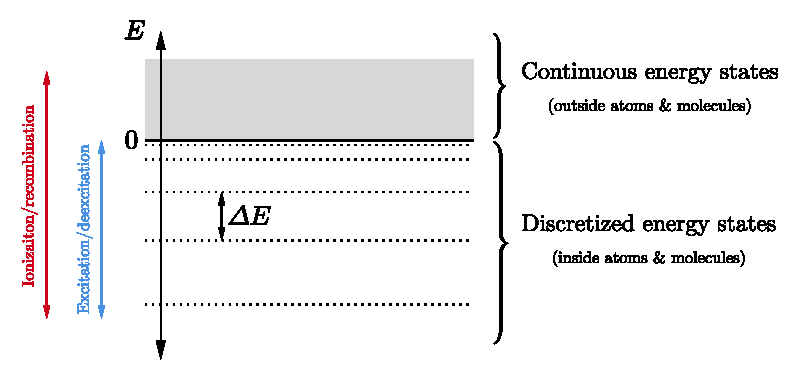
\includegraphics[width=12cm]{figures/energystates.pdf}
\caption{Illustration of discretized and continuous energy states of electrons in matter. Note, that the dotted lines for negative energies represent possible energy states within an atom or molecule (bound states), whereas \fc{the grey shaded area represents a continuum of possible energy states for free electrons.}}
\label{fig:energylevels}
\end{figure}

Consider now \cref{fig:spectrallineformation}.
\begin{figure}[h]
\centering
\includegraphics[width=10cm]{figures/spectrallineformation.pdf}
\caption{Illustration of a spectral line formation using the Eddington-Barbier relation as an explanatory tool. Note, that in this picture one assumes, that the extinction coefficient $\alpha_\lambda$ is independent of depth $z$ and furthermore, that the source function $S_\lambda = S$ is independent of wavelength and linear in $z$. This means, that the Eddington-Barbier relation does not only hold approximatively, but exactly. Moreover, the optical depth is then just given as $\tau_\lambda^\prime(Z) = \int_{0}^{Z}\alpha_\lambda\,\mathrm{d}z = \alpha_\lambda Z$. Figure inspired by \cite[p.38]{Rutten.2015}.}
\label{fig:spectrallineformation}
\end{figure}
\lk{Suppose that there is} a hypothetical atom, which is such that it contains only one electron and which has only two distinct energy states available to the electron. These energy states are separated by the energy $\Delta E$ corresponding to the wavelength $\lambda_\gamma = hc/\Delta E$. Assume further, that there is some hypothetical medium consisting of only those hypothetical atoms along with an electromagnetic radiation source; and that scattering is negligible. At precisely the wavelength $\lambda_\gamma$, this hypothetical medium will perfectly absorb all photons, as long as there are still some energy state changes available. This is to say, that there will be a spike in the curve of the extinction coefficient $\alpha_\lambda$, as it is shown in the top left panel of \cref{fig:spectrallineformation} - a spectral line is formed. Now, as such, the spectral line will be just a delta function; in reality however different broadening mechanisms such as Doppler or Lorentz broadening of spectral lines apply. Furthermore, there are many more than just two energy levels available to electrons in a real medium. Therefore, \cref{fig:spectrallineformation}  shows the extinction coefficient $\alpha_\lambda$ for some arbitrary, non-hypothetical medium. One can see, that the absorption line is centered at wavelength $\lambda_2$. \fc{Suppose now, that the extinction coefficient $\alpha_\lambda$ is not dependent upon height $z$, that the source function $S_\lambda = S$ is independent of wavelength and furthermore affine in $z$ as mentioned in the caption to \cref{fig:spectrallineformation}.} Taking into account the definition of the optical depth $\tau_\lambda^\prime(Z) = \int_{0}^{Z}\alpha_\lambda \,\mathrm{d}z$, one deduces $\tau_{\lambda_1}^\prime(z) = \alpha_{\lambda_1}z$ and $\tau_{\lambda_2}^\prime(z) = \alpha_{\lambda_2}z$. Since $\alpha_{\lambda_1} \gg \alpha_{\lambda_2}$, clearly $\tau_{\lambda_1}^\prime$ must be a steeper function of $z$ than $\tau_{\lambda_2}^\prime$. This is to say, that the medium is more opaque at wavelength $\lambda_2$ than at wavelength $\lambda_1$. Taking into account now the Eddington-Barbier relation, which states that the source function $S_\lambda$ at optical depth $\tau_\lambda^\prime= 1$ is equal to the outward spectral radiance $I_\lambda^+(0)$, one arrives at a spectral line in emission for an observer measuring $I_\lambda^+(0)$. If however, $\alpha_\lambda$ would have a spike upwards, the spectral line would appear in absorption for an observer at $\tau_\lambda^\prime = 0$.

A study of spectral line properties and an analysis, which parameters and how they influence spectral line formation can lead to insights about the medium in which they form. Using the theory of radiative transfer and especially simplified atmospheric models of stars for example, one can infer physical properties of an atmosphere simply by investigating one or more spectral lines formed in the atmosphere under consideration.
% See script of Rutten, solar spectrum formation

\section{Polarimetry}
The subject of polarimetry deals with the polarization properties of electromagnetic waves and how they are affected by the properties of the media they are propagating in. In particular, the presence of a magnetic field in the propagating medium of electromagnetic waves leads to the so-called Zeeman splitting of spectral lines, from which the presence and magnitude of a magnetic field can be deduced. Polarimetry furthermore links observable quantities like the Stokes parameters to the parameters of spectral lines, thus providing insight to the medium, where those spectral lines form. In the context of stellar atmospheres, polarimetry provides the link between the observable Stokes parameters and the parameters defining the stellar atmosphere, such as the magnetic field strength, inclination and azimuth.
% See slides and book of Landi

\subsection{Zeeman effect}
The Zeeman effect for strong external magnetic fields allows inference about the external magnetic field strength. The presence of such an external magnetic field leads to the splitting of energy levels in atoms and molecules \fc{as visualized in \cref{fig:zeemaneffect}.}
\begin{figure}[h]
	\centering
	\includegraphics[width=0.7\textwidth]{figures/zeemaneffect.pdf}
	\caption{Visualization of the Zeeman effect due to the presence of an external magnetic field $\vect{B} \neq 0$. Energy levels split into several sub-levels, if an external magnetic field is present.}
	\label{fig:zeemaneffect}
\end{figure}
This is to say, that a spectral line splits into several spectral lines, if there is a strong external magnetic field present. According to \cite[p.123]{delToroIniesta.2003}, the Zeeman wavelength splitting $\lambda_B$ can be quantified by means of \begin{equation}\label{eq:zeeman}
\lambda_B = \frac{\lambda^2 \nu_L}{c}, \quad \nu_L = \frac{e|\vect{B}|}{4\pi m c},
\end{equation} where $\nu_L$ is the Larmor frequency, $e$ is the elementary charge, $m$ is the particle mass, $\lambda$ is the wavelength of a spectral line in an inertial frame and $\vect{B}$ is the external magnetic field giving rise to the Zeeman splitting. These formulae can be derived by a rigorous calculation involving perturbation theory in quantum mechanics.
% See slides and book of Landi, possibly also del Toro Iniesta section 8.3 or Griffiths.

\subsection{The Stokes parameters and Stokes vector}
Consider a monochromatic electromagnetic wave $\vect{E}$. In general, $\vect{E}$ is a function of position $\vect{r} \in \mathbb{R}^3$ in \lk{E}uclidean space and time $t$, such that $\vect{E} = \vect{E}(\vect{r},t)$. Without loss of generality, the propagation direction of the monochromatic electromagnetic wave can be defined in $z$-direction, hence \cite[p.121]{Stix.2002} gives a monochromatic wave or arbitrary polarization state as \begin{equation}\label{eq:E-wave}
\vect{E}(\vect{r},t) = \begin{pmatrix}
E_x \cos(k z - \omega t) \\ E_y \cos(kz-\omega t + \xi) \\ 0
\end{pmatrix}, \qquad k = \frac{2\pi}{\lambda}.
\end{equation} The quantity $\xi$ is the phase difference between the amplitude of the electromagnetic wave in $x$-direction and $y$-direction, which together with $E_x$ and $E_y$ therefore accounts for the polarization state of the wave. As a side note, notice that the dispersion relation $\omega = \omega(k)$ for a wave propagating in vacuum can be given as $\omega(k) = 2\pi\nu = ck$. For the above specified electromagnetic wave, the Stokes parameters $I$, $Q$, $U$ and $V$ are defined as \begin{equation}
\vect{I} = \begin{pmatrix}
I \\ Q \\ U \\ V
\end{pmatrix} = \begin{pmatrix}
E_x^2 + E_y^2 \\ E_x^2 - E_y^2 \\ 2E_xE_y\cos(\xi) \\ 2E_xE_y\sin(\xi)
\end{pmatrix},
\end{equation} as given in \cite[p.121]{Stix.2002}. Hereby, the identity $I^2 = Q^2 + U^2 + V^2$ holds, as it is shown by the calculation \begin{align}
\begin{aligned}
Q^2 + U^2 + V^2 &= E_x^4 - 2E_x^2E_y^2 + E_y^4 + 4E_x^2E_y^2\left[\cos^2(\xi) + \sin^2(\xi)\right] \\
&= E_x^4 + 2E_x^2E_y^2 + E_y^4 = (E_x^2+E_y^2)^2 = I^2.
\end{aligned}
\end{align} \fc{Note however, that this relation only holds for completely monochromatic light, as it was derived under this assumption.} The Stokes parameters therefore are in general functions of wavelength; the wavelength dependency of $\vect{I} = \vect{I}(\lambda)$ shall henceforth be indicated by the subscript $\lambda$, such that the Stokes parameters are denoted by \begin{equation}
\vect{I}(\lambda) = \vect{I}_\lambda = (I_\lambda, Q_\lambda, U_\lambda, V_\lambda)^\top,
\end{equation} which is called the Stokes vector, whereby also $I_\lambda^2 = Q_\lambda^2 + U_\lambda^2 + V_\lambda^2$ holds. In \cref{fig:stokesvector}, a schematic representation of the definition of the Stokes parameters (vector) is given. Stokes $Q_\lambda$ and $U_\lambda$ are a measure of linear polarization, while Stokes $V_\lambda$ accounts for the amount of circular polarization present in the electromagnetic waves under consideration.
\begin{figure}[h]
\centering
\includegraphics[width=4.5cm]{figures/stokesvector.pdf}
\caption{Schematic representation of the general Stokes vector $\vect{I}_\lambda$ containing the Stokes parameters $I_\lambda$, $Q_\lambda$, $U_\lambda$ and $V_\lambda$. The observer is looking into negative $z$-direction with respect to the electromagnetic wave as defined by \cref{eq:E-wave}. Figure inspired by \cite[p.17]{DeglInnocenti.2005}.}
\label{fig:stokesvector}
\end{figure}

\subsection{The generalized radiative transfer equation}
In the preceding \lk{sections}, the radiative transfer equation was already derived and solved for the spectral radiance $I_\lambda(\tau_\lambda^\prime, \theta)$ as a function of the continuum optical depth $\tau_\lambda^\prime$ and local inclination $\theta$ of an electromagnetic radiation ray. This radiative transfer equation was given by \begin{equation}
\cos(\theta)\frac{\mathrm{d}I_\lambda(\tau_\lambda^\prime)}{\mathrm{d}\tau_\lambda^\prime} = I_\lambda(\tau_\lambda^\prime)-S_\lambda(\tau_\lambda^\prime).
\end{equation} This equation can be generalized to account not only for changes of the spectral radiance (intensity) $I_\lambda$, but for changes of every Stokes parameter $\vect{I}_\lambda = (I_\lambda, Q_\lambda, U_\lambda, V_\lambda)^\top$. This can be done by means of introducing a propagation matrix $\matr{K}_\lambda(\tau_\lambda^\prime) = \mathds{1} + \matr{N}_\lambda(\tau_\lambda^\prime)$, where $\matr{N}_\lambda(\tau_\lambda^\prime)$ accounts for extinction and emission properties of the medium giving rise to spectral line formation; and where $\mathds{1}$ is the unity matrix. Using the wavelength-dependent propagation matrix $\matr{K}_\lambda$, the generalized radiative transfer equation for the Stokes vector can be written as \begin{equation}\label{eq:generalizedradtransfereq}
\frac{\mathrm{d}\vect{I}_\lambda(\tau_\lambda^\prime)}{\mathrm{d}\tau_\lambda^\prime} = \matr{K}_\lambda(\tau_\lambda^\prime)\left[\vect{I}_\lambda(\tau_\lambda^\prime)-\vect{S}_\lambda(\tau_\lambda^\prime)\right],
\end{equation} as given by \cite[p.150]{delToroIniesta.2003}. Note that the factor of $\cos(\theta)$ is absorbed into the propagation matrix $\matr{K}_\lambda$ in the above equation. In the above formulation of the generalized radiative transfer equation also the source function $S_\lambda(\tau_\lambda^\prime)$ was generalized to the source function vector $\vect{S}_\lambda(\tau_\lambda^\prime) = S_\lambda(\tau_\lambda^\prime)(1,0,0,0)^\top$. \fc{The unity matrix} $\mathds{1}$ of the propagation matrix takes care of extinction and emission in the continuum, while the matrix $\matr{N}_\lambda$ takes into account extinction and emission pertaining to spectral lines. 
% Sections 7.6 & 7.7 in del Toro Iniesta

\subsubsection{Formal solution of the generalized radiative transfer equation}
In order to derive a formal solution to the generalized radiative transfer equation following the treatment in \cite[pp.152-157]{delToroIniesta.2003}, the parameter $\kappa \doteq \tau_\lambda^\prime$ shall be introduced to temporarily simplify the notation, hence yielding the generalized radiative transfer equation to be \begin{equation}\label{eq:generalizedradtransferkappa}
\frac{\mathrm{d}\vect{I}_\lambda(\kappa)}{\mathrm{d}\kappa} = \matr{K}_\lambda(\kappa)\left[\vect{I}_\lambda(\kappa)-\vect{S}_\lambda(\kappa)\right].
\end{equation} Consider now for the moment only the homogeneous differential equation \begin{equation}\label{eq:homogeneralizedradeq}
\frac{\mathrm{d}\vect{I}_{\lambda,h}(\kappa)}{\mathrm{d}\kappa} = \matr{K}_\lambda(\kappa)\vect{I}_{\lambda,h}(\kappa).
\end{equation} As it is done in \cite[p.152]{delToroIniesta.2003}, a so-called evolution operator $\matr{P}(\kappa, \kappa^\prime)$ can be defined, such that it gives the transformation $\vect{I}_{\lambda,h}(\kappa^\prime)\rightarrow \vect{I}_{\lambda,h}(\kappa)$ of the solution $\vect{I}_{\lambda,h}(\kappa^\prime)$ to the homogeneous equation from position $\kappa^\prime$ to $\kappa$, i.e. \begin{equation}\label{eq:evoloperatordef}
\vect{I}_{\lambda,h}(\kappa) = \matr{P}(\kappa,\kappa^\prime)\vect{I}_{\lambda,h}(\kappa^\prime).
\end{equation} This operator is linear, because the differential equation governing $\vect{I}_{\lambda,h}(\kappa)$ is also linear. Furthermore, because of the way it was defined, it has the properties \begin{gather}
\matr{P}(\kappa,\kappa) = \mathds{1}, \qquad \matr{P}(\kappa,\kappa^\prime)\matr{P}(\kappa^\prime, \kappa^{\prime\prime}) = \matr{P}(\kappa,\kappa^{\prime\prime}). 
\end{gather} Differentiating \cref{eq:evoloperatordef} with respect to $\kappa$, namely \begin{align}
\begin{aligned}
\frac{\mathrm{d}\vect{I}_{\lambda,h}(\kappa)}{\mathrm{d}\kappa} = \frac{\mathrm{d}\matr{P}(\kappa,\kappa^\prime)}{\mathrm{d}\kappa}\vect{I}_{\lambda,h}(\kappa^\prime) = \matr{K}_\lambda(\kappa)\matr{P}(\kappa,\kappa^\prime)\vect{I}_{\lambda,h}(\kappa^\prime),
\end{aligned}
\end{align} the identity \begin{equation}\label{eq:grte_op_id_1}
\frac{\mathrm{d}\matr{P}(\kappa,\kappa^\prime)}{\mathrm{d}\kappa} = \matr{K}_\lambda(\kappa)\matr{P}(\kappa,\kappa^\prime)
\end{equation} results. Furthermore differentiating \cref{eq:evoloperatordef} with respect to $\kappa^\prime$ yields \begin{align}
\begin{aligned}
\frac{\mathrm{d}\vect{I}_{\lambda,h}(\kappa)}{\mathrm{d}\kappa^\prime} = \matr{P}(\kappa,\kappa^\prime)\frac{\mathrm{d}\vect{I}_{\lambda,h}(\kappa^\prime)}{\mathrm{d}\kappa^\prime} + \frac{\mathrm{d}\matr{P}(\kappa,\kappa^\prime)}{\mathrm{d}\kappa^\prime}\vect{I}_{\lambda,h}(\kappa^\prime) = 0.
\end{aligned}
\end{align} By means of rearranging this equation and inserting the definition of the homogeneous equation \cref{eq:homogeneralizedradeq}, \lk{the expression} \begin{align}
\begin{aligned}
\frac{\mathrm{d}\matr{P}(\kappa,\kappa^\prime)}{\mathrm{d}\kappa^\prime}\vect{I}_{\lambda,h}(\kappa^\prime) &= -\matr{P}(\kappa,\kappa^\prime)\frac{\mathrm{d}\vect{I}_{\lambda,h}(\kappa^\prime)}{\mathrm{d}\kappa^\prime} \\ &= -\matr{P}(\kappa,\kappa^\prime)\matr{K}_\lambda(\kappa^\prime)\vect{I}_{\lambda,h}(\kappa^\prime)
\end{aligned}
\end{align} obtains, wherefrom the identity \begin{equation}\label{eq:grte_op_id_2}
\frac{\mathrm{d}\matr{P}(\kappa,\kappa^\prime)}{\mathrm{d}\kappa^\prime} = -\matr{P}(\kappa,\kappa^\prime)\matr{K}_\lambda(\kappa^\prime)
\end{equation} is deduced.

Now, the generalized radiative transfer equation \cref{eq:generalizedradtransferkappa} is multiplied with the operator $\matr{P}(\kappa^\prime, \kappa)$ from the left, thus obtaining \begin{align}
\begin{aligned}
\matr{P}(\kappa^\prime,\kappa)\frac{\mathrm{d}\vect{I}_\lambda(\kappa)}{\mathrm{d}\kappa} &= \matr{P}(\kappa^\prime,\kappa)\matr{K}_\lambda(\kappa)\left[\vect{I}_\lambda(\kappa)-\vect{S}_\lambda(\kappa)\right] \\
&= \frac{\mathrm{d}}{\mathrm{d}\kappa}\left[\matr{P}(\kappa^\prime,\kappa)\vect{I}_\lambda(\kappa)\right] - \frac{\mathrm{d}\matr{P}(\kappa^\prime,\kappa)}{\mathrm{d}\kappa}\vect{I}_\lambda(\kappa) \\
&= -\frac{\mathrm{d}\matr{P}(\kappa^\prime,\kappa)}{\mathrm{d}\kappa}\left[\vect{I}_\lambda(\kappa)-\vect{S}_\lambda(\kappa)\right],
\end{aligned}
\end{align} where the identity \cref{eq:grte_op_id_2} was employed in the last step. Rearranging the above equation yields \begin{align}
\begin{aligned}
\frac{\mathrm{d}}{\mathrm{d}\kappa}\left[\matr{P}(\kappa^\prime,\kappa)\vect{I}_\lambda(\kappa)\right] = \frac{\mathrm{d}\matr{P}(\kappa^\prime,\kappa)}{\mathrm{d}\kappa}\vect{S}_\lambda(\kappa) = -\matr{P}(\kappa^\prime,\kappa)\matr{K}_\lambda(\kappa)\vect{S}_\lambda(\kappa),
\end{aligned}
\end{align} where again identity \cref{eq:grte_op_id_2} was made use of. One has now an integratable equation with respect to $\kappa$. Integrating the left hand side of the above equation from $\kappa_0$ to $\kappa_1$ gives \begin{align}
\begin{aligned}
\int_{\kappa_0}^{\kappa_1}\frac{\mathrm{d}}{\mathrm{d}\kappa}\left[\matr{P}(\kappa^\prime,\kappa)\vect{I}_\lambda(\kappa)\right]\,\mathrm{d}\kappa &= \matr{P}(\kappa^\prime,\kappa_1)\vect{I}_\lambda(\kappa_1) - \matr{P}(\kappa^\prime,\kappa_0)\vect{I}_\lambda(\kappa_0) \\
&= -\int_{\kappa_0}^{\kappa_1}\matr{P}(\kappa^\prime,\kappa)\matr{K}_\lambda(\kappa)\vect{S}_\lambda(\kappa)\,\mathrm{d}\kappa.
\end{aligned}
\end{align} Through rearrangement of the equation and multiplication with $\matr{P}(\kappa_1,\kappa^\prime)$, the expressions \begin{align}
\begin{aligned}
\matr{P}(\kappa_1,\kappa^\prime)\matr{P}(\kappa^\prime,\kappa_1)\vect{I}_\lambda(\kappa_1) &= \matr{P}(\kappa_1,\kappa^\prime)\matr{P}(\kappa^\prime,\kappa_0)\vect{I}_\lambda(\kappa_0) \\
&\quad - \int_{\kappa_0}^{\kappa_1}\matr{P}(\kappa_1,\kappa^\prime)\matr{P}(\kappa^\prime,\kappa)\matr{K}_\lambda(\kappa)\vect{S}_\lambda(\kappa)\,\mathrm{d}\kappa,
\end{aligned}
\end{align} results, which can - due to the relations $\matr{P}(\kappa,\kappa^\prime)\matr{P}(\kappa^\prime,\kappa) = \matr{P}(\kappa,\kappa) = \mathds{1}$ and $\matr{P}(\kappa^{\prime\prime},\kappa^\prime)\matr{P}(\kappa^\prime,\kappa) = \matr{P}(\kappa^{\prime\prime},\kappa)$ - \fc{be further} simplified to a first formal solution to the generalized radiative transfer equation, namely \begin{equation}
\vect{I}_\lambda(\kappa_1) = \matr{P}(\kappa_1,\kappa_0)\vect{I}_\lambda(\kappa_0)- \int_{\kappa_0}^{\kappa_1}\matr{P}(\kappa_1,\kappa)\matr{K}_\lambda(\kappa)\vect{S}_\lambda(\kappa)\,\mathrm{d}\kappa.
\end{equation} Resubstituting $\tau_\lambda^\prime = \kappa$ and hence $\mathrm{d}\kappa = \mathrm{d}\tau_\lambda^\prime$, furthermore identifying $\kappa_0 = \tau_{\lambda,0}^\prime \rightarrow \infty$ and $\kappa_1 = \tau_{\lambda,1}^\prime\rightarrow \tau_\lambda^\prime$, one gets the general formal solution \begin{align}\begin{aligned}\label{eq:general_sol_gen_rad_transf_eq}
\vect{I}_\lambda(\tau_\lambda^\prime) = \matr{P}\left(\tau_\lambda^\prime,\infty\right)\vect{I}_\lambda(\infty)  -\int_{\infty}^{\tau_\lambda^\prime}\matr{P}\left(\tau_\lambda^\prime,t\right)\matr{K}_\lambda(t)\vect{S}_\lambda(t)\,\mathrm{d}t
\end{aligned}\end{align} to the generalized radiative transfer equation. Considering \cref{fig:outward-inward-radiation}, the optical depth $\tau_\lambda^\prime \rightarrow \infty$ can be understood to be located at the limit, where no photon can ever escape, e.g. at the center of a star, whose radiative transfer is described by \cref{eq:general_sol_gen_rad_transf_eq}. Further taking a closer look at \cref{fig:outward-inward-radiation}, the optical depth $\tau_\lambda^\prime = 0$ can be understood as the position of an observer located outside or right at boundary of the radiative transfer system, that is for example the position of an observer looking at a stellar atmosphere from outside the atmosphere. In this case, the measurable Stokes vector at the position of an observer outside the radiative transfer system is given as \begin{align}\begin{aligned}\label{eq:special_sol_gen_rad_transf_eq}
\vect{I}_\lambda(\tau_\lambda^\prime = 0) = \int_{0}^{ \infty}\matr{P}\left(0,t\right)\matr{K}_\lambda(t)\vect{S}_\lambda(t)\,\mathrm{d}t.
\end{aligned}\end{align} This result is obtained from \cref{eq:general_sol_gen_rad_transf_eq}, where \cite[p.153]{delToroIniesta.2003} gives the limit of the evolution operator $\matr{P}(0,t)$ for $t\rightarrow \infty$ to be \begin{equation}
\lim_{t\rightarrow \infty} \matr{P}(0,t) = 0.
\end{equation} This result makes sense insofar, as this limit can be represented as $\vect{I}_{\lambda,h}(0) = \matr{P}(0,\infty)\vect{I}_{\lambda,h}(\infty)$ by means of using the definition \cref{eq:evoloperatordef} of the evolution operator; it should account for the change in $\vect{I}_{\lambda,h}$ from $\tau_\lambda^\prime \rightarrow \infty$ to $\tau_\lambda^\prime = 0$. Since the solution $\vect{I}_{\lambda,h}$ to the homogeneous radiative transfer equation \cref{eq:homogeneralizedradeq} does not contain any source term, the homogeneous solution must change to zero as one goes from optical depth infinity to optical depth zero. This is because in this case, a ray travels a theoretically infinite distance through the radiative transfer system without any sources along the way, therefore extincting all photons on the way to optical depth zero.
% Section 9.2 in del Toro Iniesta

\subsection{Absorption, emission and dispersion profile functions}
Absorption can be defined as the removal of energy from an electromagnetic field by interaction with matter \cite[p.87]{delToroIniesta.2003}. Emission however, is the opposite of absorption, namely contribution of energy to an electromagnetic field by means of photons emerging from electronic transitions in atoms and molecules. There is a third effect due to the interaction of matter with electromagnetic fields, namely dispersion; \cite[p.87]{delToroIniesta.2003} defines it as the dephasing of the electric field components as the radiation propagates through matter.

Spectral lines due to absorption and emission properties of matter can be accounted for by so-called profile functions. These functions are not just delta functions, as the discrete energy levels in atoms and molecules would suggest, but are always broadened by different processes. Among these processes are the so-called pressure broadening (Lorentz broadening) and the thermal broadening (Doppler broadening). Doppler broadening is caused by the thermal velocities of atoms and molecules in matter, which move in arbitrary directions in general. These effects are accounted for by distinct profile functions; these two profile functions can however be combined to account for both pressure and thermal broadening by means of the mathematical operation of a convolution; thus yielding the Voigt profile function $H(u,a)$ as \begin{equation}\label{eq:Voigt_Profile}
H(u,a) = \frac{a}{\pi}\int_{-\infty}^{\infty}e^{-y^2}\frac{1}{(u-y)^2+ a^2}\,\mathrm{d}y, \end{equation} as given by \cite[p.100]{delToroIniesta.2003}. Furthermore, the dispersion effects are accounted for by the Faraday-Voigt function $F(u,a)$ given by \begin{equation}\label{eq:Faraday_Voigt_Profile}
F(u,a) = \frac{1}{\pi}\int_{-\infty}^{\infty}e^{-y^2}\frac{u-y}{(u-y)^2+a^2}\,\mathrm{d}y.
\end{equation} The Voigt and the Faraday-Voigt profile functions are visualized in \cref{fig:profilefunctions}.
\begin{figure}[h]
\centering
\begin{subfigure}[t]{0.49\textwidth}
    \centering
    \includegraphics[width=\textwidth]{figures/voightprofile.pdf}
    \caption{Voigt profile function for $a=1$.}
    \label{fig:voightprofile}
\end{subfigure}
\hfill
\begin{subfigure}[t]{0.49\textwidth}
    \centering
    \includegraphics[width=\textwidth]{figures/voightfaradayprofile.pdf}
    \caption{Faraday-Voigt profile function for $a=1$.}
    \label{fig:faradayvoightprofile}
\end{subfigure}
\caption{Voigt and Faraday-Voigt profile functions for $a=1$.}
\label{fig:profilefunctions}
\end{figure}

\subsection{The propagation matrix}\label{sec:propagationmatrix}
The propagation matrix $\matr{K}_\lambda(\tau_\lambda^\prime)$ accounts for absorption and dispersion effects of electromagnetic waves in matter within the framework of the generalized radiative transfer equation. In particular, it accounts for spectral lines in a radiation continuum. Explicitly, \cite[p.154]{Stix.2002} gives the propagation matrix to be defined as \begin{equation}
\matr{K}_\lambda = \begin{pmatrix}
\eta_I & \eta_Q & \eta_U & \eta_V \\
\eta_Q & \eta_I & \rho_V & -\rho_U \\
\eta_U & -\rho_V & \eta_I & \rho_Q \\
\eta_V & \rho_U & -\rho_Q & \eta_I
\end{pmatrix}.
\end{equation} \cite[p.116]{delToroIniesta.2003} \lk{gives the individual entries of this matrix as} \begin{align}\begin{aligned}
\eta_I &= 1 + \frac{\eta_0}{2}\left[\phi_0\sin^2(\theta) + \frac{1}{2}(\phi_{+1}+\phi_{-1})(1+\cos^2(\theta))\right], \\
\eta_Q &= \frac{\eta_0}{2}\left[\phi_0-\frac{1}{2}(\phi_{+1}+\phi_{-1})\right]\sin^2(\theta)\cos(2\varphi), \\
\eta_U &= \frac{\eta_0}{2}\left[\phi_0 - \frac{1}{2}(\phi_{+1}+\phi_{-1})\right]\sin^2(\theta)\sin(2\varphi), \\
\eta_V &= \frac{\eta_0}{2}(\phi_{-1}-\phi_{+1})\cos(\theta), \\
\rho_Q &= \frac{\eta_0}{2}\left[\psi_0-\frac{1}{2}(\psi_{+1}+\psi_{-1})\right]\sin^2(\theta)\cos(2\varphi), \\
\rho_U &= \frac{\eta_0}{2}\left[\psi_0-\frac{1}{2}(\psi_{+1}+\psi_{-1})\right]\sin^2(\theta)\sin(2\varphi), \\
\rho_V &= \frac{\eta_0}{2}(\psi_{-1}-\psi_{+1})\cos(\theta).
\end{aligned}
\end{align} Hereby, the angles $\theta$ and $\varphi$ are called inclination and azimuth and are defined as seen in \cref{fig:inclinationazimuth}. \begin{figure}[h]
\centering
\includegraphics[width=8cm]{figures/inclinationazimuth.pdf}
\caption{Visualization of the definitions for the inclination and azimuth angles $\theta$ and $\varphi$.}
\label{fig:inclinationazimuth}
\end{figure} The ranges for those angles are $\theta \in [0,\pi]$ and $\varphi \in [0,2\pi]$. \fc{Note, that inversion codes for solar observations exhibit a \ang{180} ambiguity, since it cannot be determined from the Stokes parameter alone, if the magnetic field points towards $\varphi = \pi/2$ or $\varphi = 3\pi/4$, for example. This is in particular the case for the Milne-Eddington inversion code used in this thesis}. In the case of solar observations, $\theta = 0$ means that a vector field $\vect{V}$ under consideration is oriented towards an observer on-looking the Sun, whereas $\varphi=0$ does either mean, that the vectorial quantity $\vect{V}$ \lk{faces either perfectly north or east on the solar surface, depending on the convention used by some author. In the experiments conducted for this thesis however, $\varphi = 0$ is identified with solar north, where the azimuth value $\varphi$ increases in clockwise direction}. $\theta=\pi$ then does mean, that $\vect{V}$ points exactly away from the observer.

The quantities $\phi_\alpha$ and $\psi_\alpha$ for $\alpha \in \{0,-1,1\}$ are left to be defined; \cite[p.123]{delToroIniesta.2003} defines these parameters as \begin{align}
\begin{aligned}
\phi_\alpha(u,a) &= \frac{1}{\sqrt{\pi}}H(u + \alpha u_B - u_{los}, a), \\
\psi_\alpha(u,a) &= \frac{1}{\sqrt{\pi}}F(u + \alpha u_B - u_{los},a).
\end{aligned}
\end{align} Herewith, $u$, $u_B$ and $u_{los}$ aswell as $a$ are dimensionless quantities determining the the Voigt and Faraday-Voigt functions. In these functions $u$ is related to the wavelength $\lambda$ and is to be regarded as a fixed value for a certain spectral line under consideration. \cite[p.21]{UitenbroekNSME.2020} gives the parameter $u_{los}$ as \begin{equation}
u_{los} = \lambda\frac{\vect{u}\cdot\vect{n}}{c\Delta\lambda_D},
\end{equation} where $\vect{n}$ defines the line of sight vector and $\vect{u}$ the velocity of the medium constituents relative to an inertial observer outside the radiative transfer system. This is a dimensionless number related to the actual line of sight velocity $v_{los}$ as $v_{los} = cu_{los}$. Furthermore, $\Delta \lambda_D$ refers to the Doppler broadening of a spectral line due to the thermal velocity \begin{equation}
v_{th} = \sqrt{\frac{2k_BT}{m}}
\end{equation} of the particles of mass $m$ in the medium; it is given by the expression \begin{equation}
\Delta \lambda_D = \frac{v_{th}\lambda}{c} = \frac{\lambda}{c}\sqrt{\frac{2k_B T}{m}}.
\end{equation} Since the thermal velocity of the particles is responsible for the Doppler broadening, one can also call the thermal velocity $v_{th}$ the Doppler velocity $v_{dop} \doteq v_{th}$. Last but not least, $u_B$ is a factor originating in the Zeeman effect; therefore it connects the radiative transfer equation with an external magnetic field $\vect{B}$ via the relation \begin{equation}
u_B = g_L\frac{e\lambda^2|\vect{B}|}{4\pi m c\Delta \lambda_D},
\end{equation} where $g_L$ is the Landé factor. In total therefore, the propagation matrix $\matr{K}_\lambda$ for a certain wavelength $\lambda$ can be fully determined by means of the seven independent parameters $\{|\vect{B}|, \theta, \varphi, v_{los}, v_{dop}, a, \eta_0\}$.
% Section 7.6 in del Toro Iniesta with
% Profile functions: (6.55)-(6.58).
% Profile functions with Zeeman effect and LOS-velocity: (8.7)-(8.13); (6.42)-(6.48).
% and also picture of azimuth and inclination angles definition with respect to line of sight.

\subsection{The Milne-Eddington approximation}\label{sec:MEapproximation}
% Section 9.4.1 in del Toro Iniesta with eqs. (7.42), (7.43), (7.44), (7.45). 
% Profile functions: (6.55)-(6.58).
% Profile functions with Zeeman effect and LOS-velocity: (8.7)-(8.13); (6.42)-(6.48).
The Milne-Eddington approximation of radiative transfer allows for the construction of a relatively simple stellar atmosphere model $\vect{y} = \vect{M}(\vect{x})$, where $\vect{x}$ would be the atmospheric parameters, such as  magnetic field strength, inclination and so forth; and where $\vect{y}$ would be the predicted observational data, namely the Stokes vectors $\vect{I}_\lambda$ for a certain wavelength interval $\lambda \in [\lambda_-,\lambda_+]$ giving so-called Stokes profiles. A Milne-Eddington model for a stellar atmosphere can even be analytically inverted, which means that there is a mathematically exact way to calculate atmospheric parameters $\vect{x}$ based on observational data $\vect{y}$ by means of mathematically inverting the model, i.e. $\vect{x} = \vect{M}^{-1}(\vect{y})$. In the case of real and not synthetic observational data $\vect{y}$, the best fit to the data given the model $\vect{y} = \vect{M}(\vect{x})$ is to be found by iteratively changing the parameters; that is by means of synthesizing observations, comparing them to the real observations and adjusting the parameters, such that a better fit to the real observations is expected in the next iteration.

The simplest possible solution for the generalized radiative transfer equation \cref{eq:generalizedradtransfereq} is the so-called Milne-Eddington solution. Its derivation relies on the Milne-Eddington approximation, which basically consists of three fundamental assumptions given in \cite[p.411]{DeglInnocenti.2005} profoundly simplifying the radiative transfer problem:
\begin{enumerate}
\item The radiative transfer system is assumed to be of a plane parallel nature and in a local thermodynamic equilibrium.
\item All parameters relevant to spectral line formation are required to be independent of all measures of height within the system.
\item The source function is required to be affinely dependent upon the continuum optical depth.
\end{enumerate}

The second assumption is to say, that the propagation matrix $\matr{K}_\lambda$ is isotropically constant, i.e. \begin{equation}
\matr{K}_\lambda = \matr{K}_{\lambda,0},
\end{equation} \fc{where the subscript $\lambda,0$ indicates, the propagation matrix does not depend on any measure of height within the described atmosphere, but still on $\lambda$.} The third ingredient to the Milne-Eddington model means, that the source function vector can be written as \begin{equation}
\vect{S}_\lambda(\tau_\lambda^\prime) = \vect{S}_{\lambda,0} + \tau_\lambda^\prime \vect{S}_{\lambda,1},
\end{equation} where $\vect{S}_{\lambda,0} = S_{\lambda,0}(1,0,0,0)^\top$ and $\vect{S}_{\lambda,1}=S_{\lambda,1}(1,0,0,0)^\top$ are constant vectors. Using the first assumption of the Milne-Eddington model, one can furthermore make the identifications $S_{\lambda,0} = B_\lambda(T)$ and $S_{\lambda,1} = B_\lambda(T)\beta$ with $\beta \in \mathbb{R}$ a constant. This is because local thermodynamic equilibrium implies, that the source function is locally equal to the Planck function. \fc{The parameter $\beta$ is a measure on how rapidly the source function $\vect{S}_\lambda(\tau_\lambda^\prime)$ changes with increasing optical depth $\tau_\lambda^\prime$ in the stellar atmosphere. For high positive values of $\beta$, there is a strong increase in intensity for the source function with increasing optical depth, whereas for $\beta=0$, the source function would be independent of optical depth.}

In the Milne-Eddington case, the homogeneous generalized radiative transfer equation \cref{eq:homogeneralizedradeq} reads as \begin{equation}
\frac{\mathrm{d}\vect{I}_{\lambda,h}(\tau_\lambda^\prime)}{\mathrm{d}\tau_\lambda^\prime} = \matr{K}_{\lambda,0}\vect{I}_{\lambda,h}(\tau_\lambda^\prime).
\end{equation} According to standard mathematical literature, the matrix exponential $e^{\matr{A}}$ for a matrix $\matr{A}$ is defined as \begin{equation}
e^{\matr{A}} = \mathds{1} + \matr{A} + \frac{1}{2!}\matr{A}^2 + \frac{1}{3!}\matr{A}^3 + \dots = \sum_{k=1}^{\infty}\frac{\matr{A}^k}{k!},
\end{equation} Analogously to the scalar case \lk{therefore}, a solution to the generalized homogeneous radiative transfer equation can be given as \begin{equation}
\vect{I}_\lambda(\tau_\lambda^\prime = 0) = e^{-\matr{K}_{\lambda,0}\tau_\lambda^\prime}\vect{I}_\lambda(\tau_\lambda^\prime).
\end{equation} Comparing this to the definition \cref{eq:evoloperatordef} of the evolution operator, one finds \begin{equation}
\matr{P}(0,\tau_\lambda^\prime) = e^{-\matr{K}_{\lambda,0}\tau_\lambda^\prime}
\end{equation} in the Milne-Eddington case. One can now calculate the solution $\vect{I}_\lambda(\tau_\lambda^\prime=0, \theta)$ using the special case \cref{eq:special_sol_gen_rad_transf_eq} of the formal solution to the generalized radiative transfer equation, namely 
\begin{equation}
\vect{I}_\lambda(\tau_\lambda^\prime = 0,\theta) = \int_{0}^{ \infty}\matr{P}\left(0,t\right)\matr{K}_\lambda(t)\vect{S}_\lambda(t)\,\mathrm{d}t.
\end{equation}
First, note that the derivative of $e^{-\matr{K}_{\lambda,0}\tau_\lambda^\prime}$ is given by \begin{equation}
\frac{\mathrm{d}}{\mathrm{d}\tau_\lambda^\prime}e^{-\matr{K}_{\lambda,0}\tau_\lambda^\prime} = -e^{-\matr{K}_{\lambda,0}\tau_\lambda^\prime}\matr{K}_{\lambda,0},
\end{equation} because \begin{align}
\begin{aligned}
\frac{\mathrm{d}}{\mathrm{d}x}e^{x\matr{A}} &= \frac{\mathrm{d}}{\mathrm{d}x}\left(\mathds{1} + x\matr{A} + \frac{1}{2!}x^2\matr{A}^2 + \frac{1}{3!}x^3\matr{A}^3 + \dots \right) \\
&= \matr{A} + x\matr{A}^2 + \frac{1}{2!}x^2\matr{A}^3 +  \frac{1}{3!}x^3\matr{A}^4 + \dots \\
&= \left(\mathds{1} + x\matr{A} + \frac{1}{2!}x^2\matr{A}^2 +  \frac{1}{3!}x^3\matr{A}^3 + \dots\right)\matr{A} = e^{x\matr{A}}\matr{A},
\end{aligned}
\end{align} hence consequently also $\frac{\mathrm{d}}{\mathrm{d}x}e^{-x\matr{A}} = -e^{x\matr{A}}\matr{A}$ holds for any matrix $\matr{A}$ and real parameter $x$. Therefore, $-e^{-\matr{K}_{\lambda,0}\tau_\lambda^\prime}\matr{K}_{\lambda,0}^{-1}$ is an antiderivative of $-e^{-\matr{K}_{\lambda,0}\tau_\lambda^\prime}$. Now, one proceeds by calculating \begin{align}
\begin{aligned}\label{eq:fundamentalMEsolution}
\vect{I}_\lambda(\tau_\lambda^\prime = 0) &= \int_{0}^{ \infty}\matr{P}\left(0,t\right)\matr{K}_\lambda(t)\vect{S}_\lambda(t)\,\mathrm{d}t \\ &= \int_{0}^{\infty}\underbrace{e^{-\matr{K}_{\lambda,0}t}\matr{K}_{\lambda,0}}_{\doteq\,\tfrac{\mathrm{d}}{\mathrm{d}t}\matr{F}(t)}\underbrace{\left(\vect{S}_{\lambda,0}+t\vect{S}_{\lambda,1}\right)}_{\doteq\,\vect{G}(t)}\,\mathrm{d}t \\
&= \left[\matr{F}(t)\vect{G}(t)\right]^{\infty}_{0} - \int_{0}^{\infty} \matr{F}(t)\frac{\mathrm{d}}{\mathrm{d}t}\vect{G}(t)\,\mathrm{d}t \\
&= \left[-e^{-\matr{K}_{\lambda,0}t}\matr{K}_{\lambda,0}^{-1}\matr{K}_{\lambda,0}(\vect{S}_{\lambda,0}+t\vect{S}_{\lambda,1})\right]^{\infty}_{0} \\ &\quad + \int_{0}^{\infty}e^{-\matr{K}_{\lambda,0}t}\matr{K}_{\lambda,0}^{-1}\matr{K}_{\lambda,0}\vect{S}_{\lambda,1}\,\mathrm{d}t \\
&= \vect{S}_{\lambda,0} + \int_{0}^{\infty}e^{-\matr{K}_{\lambda,0}t}\vect{S}_{\lambda,1}\,\mathrm{d}t \\ &= \vect{S}_{\lambda,0} + \left[e^{-\matr{K}_{\lambda,0}t}\matr{K}_{\lambda,0}^{-1}\vect{S}_{\lambda,1}\right]^{\infty}_0 \\ &= \vect{S}_{\lambda,0}-\matr{K}_{\lambda,0}^{-1}\vect{S}_{\lambda,1}.
\end{aligned}
\end{align} As stated by \cite[p.160]{delToroIniesta.2003}, this is the fundamental result of the Milne-Eddington approximation and is sometimes also called the Unno-Rachkovsky solution. \fc{Note, that $\lambda$ refers to the central wavelength of the considered spectral line(s). The parameters defining the Milne-Eddington atmosphere are considered to be constant for a considered wavelength window centered around $\lambda$, such that the algorithm converges to a unique solution per observation.} Identifying therefore $\vect{S}_{\lambda,0} = S_{\lambda,0}(1,0,0,0)^\top = S_0(1,0,0,0)^\top$ and $\vect{S}_{\lambda,1} = S_{\lambda,1}(1,0,0,0)^\top = S_1(1,0,0,0)^\top$ and taking into account, that the propagation matrix $\matr{K}_{\lambda,0}$ depends upon the seven parameters as specified in \cref{sec:propagationmatrix}, the Stokes values $\vect{I}_\lambda(\tau_\lambda^\prime =0)$ around the central wavelength $ $ of a spectral line are determined fully by the set  of nine parameters $|\vect{B}|$, $\theta$, $\varphi$, $v_{los}$, $v_{dop}$, $a$, $\eta_0$, $S_0$, $S_1$; \lk{see \cref{tab:paramsummary} for a concise summary of these parameters and their meaning.}
\begin{table}[h]
\centering
\begin{tabularx}{\textwidth}{|c|X|}
\hline
\textbf{Parameter} & \textbf{Explanation} \\
\hline\hline
$|\vect{B}|$ & Magnitude of the magnetic field vector. \\
\hline
$\theta$ & Inclination value of the magnetic field vector. $\theta=0$ means orientation of the magnetic field towards the observer, $\theta = \pi$ away from the observer.\\
\hline
$\varphi$ & Azimuth value of the magnetic field vector. $\varphi=0$ means orientation of the magnetic field towards solar north, $\varphi = \pi/2$ towards solar east.\\
\hline
$v_{los}$ & Line of sight velocity of emitting/absorbing matter. \\
\hline
$v_{dop}$ & Doppler velocity corresponding to the Doppler broadening $\Delta \lambda_D = v_{dop}\lambda / c$ of spectral lines. \\
\hline
$a$ & Damping parameter affecting the spectral line shape. The damping is strong for high values of $a$ and vice versa. \\
\hline
$\eta_0$ & Line strength parameter for spectral lines. A spectral line is highly pronounced relative to the continuum for high values of $\eta_0$ and vice versa. \\
\hline
$S_0$ & Shift parameter for the source function as an affine function of optical depth. \\
\hline
$S_1$ & Scale parameter for the source function as an affine function of optical depth. \\
\hline
\end{tabularx}
\caption{Summary of the nine Milne-Eddington atmospheric parameters.}
\label{tab:paramsummary}
\end{table}
Note, that $S_0$ is related to the Planck function as $B_\lambda(T) = S_0$; therefore, one can also assign a temperature $T$ to the system under investigation once one has a value for $S_0$ and knows which wavelength $\lambda$ to consider\footnote{\fc{As \cite[p.281]{Froehlich.2004} note, starting from optical depth $\tau_{500}^\prime = 1$ at $\lambda = \SI{500}{\nano\meter}$, the temperature $T$ in the photosphere for quiet sun conditions decreases first from roughly $\SI{6500}{\kelvin}$ to approximately $\SI{4500}{\kelvin}$ at $\tau_{500}^\prime \approx 10^{-4}$, which marks the boundary between the photosphere and the chromosphere. Then, the temperature in the chromosphere again increases up to $\SI{7000}{\kelvin}$ at roughly $\tau_{500}^\prime \approx 10^{-6}$.}}.

The parameter vector $\vect{x}$ of the Milne-Eddington model is hence given as \begin{equation}
\vect{x} = (|\vect{B}|,\theta,\varphi,v_{los},v_{dop},a,\eta_0,S_0,S_1)^\top \in \mathbb{R}^9.
\end{equation} 
Let a number $D \in \mathbb{N}$ of wavelengths be sampled from a given wavelength interval $[\lambda_{min},\dots,\lambda,\dots,\lambda_{max}]$ centered around $\lambda$, the central wavelength of a spectral line. Therefore, the observations vector $\vect{y}$ of the Milne-Eddington model is accounted for by \begin{equation}
\vect{y} = (\vect{I}_{\lambda_{min}},\dots,\vect{I}_\lambda,\dots,\vect{I}_{\lambda_{max}})^\top \in \mathbb{R}^D.
\end{equation} 
Thus, the full Milne-Eddington model can be written as \begin{equation}\label{eq:ME_model_equation}
\vect{M}:\mathbb{R}^9 \rightarrow \mathbb{R}^D, \quad \vect{x} = \begin{pmatrix}
|\vect{B}| \\
\theta \\
\varphi \\
v_{los} \\
v_{dop} \\
a \\
\eta_0 \\
S_0 \\
S_1
\end{pmatrix} \mapsto \vect{y} = \vect{M}(\vect{x}) = \begin{pmatrix}
\vect{I}_{\lambda_{min}} \\
\vdots \\
\vect{I}_{\lambda} \\
\vdots \\
\vect{I}_{\lambda_{max}}
\end{pmatrix},
\end{equation}
where \cref{eq:fundamentalMEsolution} is identified to define the model $\vect{y} = \vect{M}(\vect{x})$.

%\subsubsection{Rough implementation of the Milne-Eddington model}
%One can implement a rough Milne-Eddington model  $\vect{y} = \vect{M}(\vect{x})$ as given in \cref{eq:ME_model_equation}. This can be done by means of exactly implementing all equations as specified in \cref{sec:MEapproximation}, e.g. in the programming language \verb|Python|. In \cref{fig:MEroughimplementation}, the results of such a rough implementation can be seen for $u = 2u_{los}$ and the parameter values \begin{gather}\begin{gathered}
%|\vect{B}| = 100.0,\ \theta = \frac{\pi}{2},\ \varphi = \frac{\pi}{2},\ v_{los}=1.0,\ v_{dop}=2.0,\ a = 0.01,\\ \eta_0 = 2.0,\ S_0 = 1.0,\ S_1 = 1.0,\ c = 1.0, \ g_L = 1.0,\ e = 1,\ m=1.
%\end{gathered}\end{gather} As is evident by closer examination, there are some quirks within these plots/results; for example, the stokes $I$ parameter becomes negative at some points, which cannot be true. Likely, these quirks can possibly be explained by numerical issues of the calculations, but further examination of these issues would be needed to either verify or discard this claim.
%\begin{figure}[h]
%\centering
%\includegraphics[width=\textwidth]{figures/MEimplementation.pdf}
%\caption{Rough implementation of the Milne-Eddington model $\vect{y} = \vect{M}(\vect{x})$ as given by \cref{eq:ME_model_equation}. Note, that the plots are given around the central wavelength $\lambda$, of a spectral line, which is set equal to zero in the plots.}
%\label{fig:MEroughimplementation}
%\end{figure}

\section{Stellar atmosphere models}
\subsection{Stellar atmosphere inversions}
Consider some observation $\vect{y}$ of a stellar atmosphere. Assume, that there is a model $\vect{M}$ with associated parameters $\vect{x}$, such that the model is given by the relationship $\vect{M} = \vect{M}(\vect{x}) = \vect{y}$.
% Make a nice graphic for this

So if one knows the parameter values $\vect{x}_0$ of the stellar atmosphere model $\vect{M}$, then observations $\vect{y}_0$ can be generated based on the parameter values $\vect{x}_0$ by means of the relation $\vect{y}_0 = \vect{M}(\vect{x}_0)$; this is called the forward model. However, if one only has observations $\vect{y}_0$ and the stellar model $\vect{M}$, one would like to find out the model parameters $\vect{x}_0$ associated to these observations; this is called the backward model and can be achieved by means of applying the relation $\vect{x}_0 = \vect{M}^{-1}(\vect{y}_0)$. As one can see, this requires a so-called inversion of the atmosphere model $\vect{M}$, which can lead to degeneracy in the model parameters $\vect{x}_0$, meaning that more than one configuration of $\vect{x}_0$ can lead to the same observations $\vect{y}_0$. A so-called normalizing flow \lk{as it will be explained in the subsequent chapter} helps to disentangle this degeneracy by means of introducing a probability density function for each model parameter, such that the more likely parameter configurations leading to some observations $\vect{y}_0$ can be distinguished from less likely parameter configurations leading to the same observations.

\subsection{Solving a stellar atmosphere inversion problem}
Consider a stellar model $\vect{M}(\vect{x})$. Given observations $\vect{y}_0$, one would like to infer the stellar parameters $\vect{x}_0$ associated to these observations by applying the relation \begin{equation}
\vect{x}_0 = \vect{M}^{-1}(\vect{y}_0).
\end{equation} Commonly, such inversion problems are carried out using a gradient search minimization algorithm which basically functions as follows. First, a function which should be minimized is defined; in our case \begin{equation}
\vect{F}(\vect{x}) \doteq \vect{M}^{-1}(\vect{y}_0) - \vect{x}.
\end{equation} By computing the gradient of $\vect{F}(\vect{x}) = (F_1(\vect{x}), \dots, F_n(\vect{x}))^\top,\,n\in\mathbb{N}$ with respect to the parameters $\vect{x}$, that is for every $F_i \in \vect{F} = (F_1,\dots,F_n)^\top$ the vector $\vect{\nabla}_{\vect{x}}F_i(\vect{x})$ is calculated, one approaches a minimum of $\|\vect{F}\|$ to be identified with $\vect{x}_0$, if $\vect{x}$ is iteratively changed in the direction of negative gradient of $\vect{F}(\vect{x})$.

\fc{However, there are significant disadvantages to such algorithms; first of all, these types of algorithms are computationally costly. A second disadvantage is that these algorithms usually return just a single vector as the approximate solution to the minimization problem. This is where} the normalizing flows technique comes into play, which provides a computationally more efficient way to do inversions and furthermore allows for the possibility to construct a probability density of possible solutions to the inversion problem. \fc{Using a trained normalizing flow, one can sample from the posterior density $p(\vect{x}_0|\vect{y}_0)$ and thus obtain a probability density for the atmospheric parameters $\vect{x}_0$, rather than just a single solution vector $\vect{x}_0$.}

\subsection{Calculation of synthesized datasets using a stellar atmosphere model}\label{sec:calcsyntheticdatasets}
\fc{Consider a case, where the stellar atmospheric parameter data $\vect{x} \in \mathbb{R}^d$ is conditioned by (synthetic) observational data $\vect{y} \in \mathbb{R}^D$ by means of a model $\vect{y} = \vect{M}(\vect{x})$. In such a case, $\vect{y}$ will be here and henceforth called ``context'' for $\vect{x}$.}
%In the case, where  data $\vect{x} \in \mathbb{R}^d$ is conditioned by context $\vect{y} \in \mathbb{R}^D$, it can be of interest to find a mathematical model implementing a transformation $\vect{y} = \vect{M}(\vect{x})$. 
In order to be able to train a normalizing flow implementing a transformation \begin{gather}
\vect{f}_{\vect{y},\vect{\phi}(\hat{\matr{x}},\hat{\matr{y}})}: \mathbb{R}^d\rightarrow \mathbb{R}^d, \quad \vect{x}\mapsto \vect{z} =  \vect{f}_{\vect{y},\vect{\phi}(\hat{\matr{x}},\hat{\matr{y}})}(\vect{x}),
\end{gather} if can be a commodity to know the true posterior distribution $p(\vect{x}|\vect{y})$, thus enabling a comparison to the posterior distribution $p_{\vect{\phi}(\hat{\matr{x}},\hat{\matr{y}})}(\vect{x}|\vect{y})$ learned by the normalizing flow; this can be done by application of the Bayes theorem. Note, that $\vect{\phi}(\hat{\matr{x}},\hat{\matr{y}})$ are weights depending upon training data $\hat{\matr{x}}$ and $\hat{\matr{y}}$ associated to the implementation of the function $\vect{f}_{\vect{y},\vect{\phi}}$ by a neural network. As to calculate the true posterior distribution by means of the model $\vect{M}(\vect{x}) = \vect{y}$ linking together the so-called context $\vect{y}$ with the input $\vect{x}$ to the normalizing flow, one can proceed as follows.

First, $\vect{x}$ is assumed to follow a specific probability density $p(\vect{x})$, for example a uniform distribution. Next, one can sample $L\in \mathbb{N}$ datapoints $\{\vect{x}_{1},\dots,\vect{x}_{L}\}$ from the prior $p(\vect{x})$. Using the model $\vect{M}$, for every $\vect{x}_{k}$ the corresponding value $\vect{y}_{k}$ can be calculated as $\vect{y}_{k} = \vect{M}(\vect{x}_{k})$, leading to the likelihood distribution $p(\vect{y}|\vect{x})$. Using the Bayes theorem and the law of total probability, one can calculate $p(\vect{x}_{k}|\vect{y}_{k})$ as \begin{equation}
p(\vect{x}_{k}|\vect{y}_{k}) = \frac{p(\vect{y}_{k}|\vect{x}_{k})p(\vect{x}_{k})}{\sum_{j=1}^{L}p(\vect{y}_{k}|\vect{x}_{j})p(\vect{x}_{j})},
\end{equation} leading to the probability distribution $p(\vect{x}|\vect{y})$ for $k \in \{1,\dots,L\}$ and $L \rightarrow \infty$.

\chapter{Artificial intelligence}
The field of artificial intelligence (AI) is \lk{a} relatively recent field of research dedicated to mimic the process of learning information. Hereby, inspiration for first principles of a sub-field of artificial intelligence, the so-called deep learning, comes from the brain structure of humans. 

As artificial intelligence tries to mimic the process of learning, it remains to be answered what learning actually is. In order to define how a learning process is constituted, another quantity has to be defined first, namely information. \cite[p.2]{Mitchell.1997} defines learning such that a computer program is said to learn from experience $E$ with respect to some class of tasks $T$ and performance measure $P$, if its performance at tasks in $T$, as measured by $P$, improves with experience $E$. If the so-called information entropy, which will be defined at a later stage, serves as a performance measure $P$, the process of learning can also be described by the statement, that any learning process decreases the information entropy of some system under consideration.

\section{Information theory}
Following \cite[p.73]{Goodfellow.2016}, the fundamental intuition of information theory is the consideration, that the occurrence of an unlikely event should convey more information than the occurrence of a likely event. The quantification of information in the field of information theory therefore relies on three key requirements, as given by \cite[p.73]{Goodfellow.2016}:
\begin{enumerate}
\item Likely events should have low information content. Guaranteed events are required to have no information content.
\item Unlikely events should have high information content.
\item Independent events should have additive information; i.e. learning about two independent events of the same likelihood should convey twice as much information as learning about the occurrence of only one of these events.
\end{enumerate} % See deep learning book and lecture

\subsection{Self-information}
The above mentioned requirements are satisfied by the so-called self-information $\mathcal{I}[p(x)]$ as defined by \cite[p.73]{Goodfellow.2016}, namely \begin{equation}\label{eq:defselfinformation}
\mathcal{I}[p(x)] = -\log\left[p(x)\right],
\end{equation} with $X$ being a random variable and $p(x)$ the probability density function thereof.

By this definition, information $\mathcal{I}[p(x=U)]$ of an unlikely event $x=U$ will be higher than information $\mathcal{I}[p(x=L)]$ of a likely event $x = L$; this can be demonstrated by assessing the self-information contents of both events. Because $U$ is said to be an unlikely event, $p(U) \approx 0$ will hold and therefore $\mathcal{I}[p(x=U)] = -\log[p(U)] = \log[1/p(U)] \gg 1$. Since $L$ is a likely event, the probability $p(L)$ of $L$ occurring is estimated by $p(L) \approx 1$ and the self-information $\mathcal{I}[p(x=L)]$ will therefore be very low, because $\mathcal{I}[p(x=L)] = -\log[p(L)] = \log[1/p(L)] \approx 0$ holds. Moreover, information about two independent events $x=A$ and $x=B$ is additive, as the calculation
\begin{align}
\begin{aligned} \mathcal{I}[p(A\cap B)] &= -\log[p(A\cap B)] = -\log[p(A)p(B)] \\ &= -(\log[p(A)] + \log[p(B)]) = \mathcal{I}[p(A)] + \mathcal{I}[p(B)]
\end{aligned}
\end{align} shows it to be the case.

\subsection{Information entropy}
One can describe the information content of a probability density function by the so-called information entropy given by \cite[p.74]{Goodfellow.2016} as
\begin{equation}
H_p[p(x)] = E_{x\sim p}(\mathcal{I}[p(x)]) = -E_{x\sim p}\left(\log[p(x)]\right),
\end{equation} where $p(x)$ is a probability density function of a random variable $X$. If the random variable $X$ is of a discrete nature, the information entropy is called Shannon entropy, whereas if $X$ is continuous, the information entropy goes by the name of differential entropy. % See deep learning book

Information entropy defined in this way is a measure of the amount of uncertainty in a probability distribution. The information entropy will be very low, if $p(x)$ describes mostly very likely events, whereas it will be very high, if $p(x)$ describes mainly very unlikely events. This can also be stated in the following way: Probability distributions that are nearly deterministic (delta-function shaped) have a low entropy, whereas distributions that are closer to a uniform distribution have high entropy.

The field of artificial intelligence and especially its sub-field machine learning are concerned with learning the available self-information from the data. That is to say, the information entropy initially present within the machine learning entity is iteratively reduced by means of training it on a dataset, thus resulting in learned information on the part of the trained artificial intelligence.

\section{Overview of artificial intelligence}
According to \cite[p.7]{Amini.2023}, the field of artificial intelligence can be broadly described as any computational technique, that enables a computer to engage with information in a reasonable way, such as to mimic how a human would process the available data or information. Machine learning is \lk{a} more specialized sub-field of artificial intelligence, which is concerned with any routine, that gives a computer the ability to learn a task without being explicitly programmed for that particular task. Deep learning, which is ultimately about reflecting and rebuilding a simple representation \lk{of} the human brain working principle, is an even more specialized sub-field of artificial intelligence, which is itself a sub-field of machine learning.

The foundational tool of deep learning is the so-called neural network, also known as deep neural network. The basic building block of a neural network is the single layer perceptron (SLP). By combining several single layer perceptrons to a multi layer perceptron (MLP), a deep neural network can be constructed. Given an input vector $\vect{x} = (x_1, \dots, x_d)^\top \in\mathbb{R}^d$ and an output vector $\bar{\vect{x}} = (\bar{x}_1,\dots,\bar{x}_w)^\top \in \mathbb{R}^w$ with $d,w \in \mathbb{N}$, the working principle of \lk{a} single layer perceptron is shown in \cref{fig:SLP}, similarly for a multi layer preceptron in \cref{fig:MLP}.

\section{Neural networks}
The ``blueprint'' of the single layer perceptron - or simply ``perceptron'' - as the building block of neural networks is inspired by the most basic structure in a human brain: The neuron. this is why a network consisting of multiple connected perceptrons is called a (deep) neural network. As the human neuron cell body collects and processes various signals originating in the dendrites and outputs some signal to the axon terminating in the axon terminals, the perceptron gathers multiple input values, calculates a weighted sum of all inputs, pushes this sum through a so-called activation function and outputs some new value. The similarity between a human neuron and the perceptron is found visualized in \cref{fig:neuronperceptron}. 
\begin{figure}[h]
\centering
\includegraphics[width=\textwidth]{figures/neuronperceptron.pdf}
\cprotect\caption{Visualization of the similarities between a human neuron and the single layer perceptron. Image credit for image in left panel: Clker-Free-Vector-Images, \url{https://www.needpix.com/photo/170704/}, accessed on January 02, 2024. Adapted by the author.}
\label{fig:neuronperceptron}
\end{figure}
The following treatment of single layer and multi layer perceptrons follows the material to be found in \cite[p.338-342]{Raschka.2022}.

% Make analogy to body neuron 
% Parallelize strands with axons, sum with sum of inpulses of axons and activation function with threshold for the neuron to fire
\subsection{Single layer perceptron}
In \cref{fig:SLP}, a single layer perceptron is visualized. The single layer perceptron generates a single output $\bar{x}$ from an input vector $\vect{x} = (x_1,\dots,x_d) \in \mathbb{R}^d$ with $d \in \mathbb{N}$. First, all input vector components $x_i$ are multiplied with initially arbitrary weights $\phi_i \in \mathbb{R}$ for all $i \in \{1,\dots,d\}$ and subsequently summed up to \lk{the sum $\tilde{s} = \sum_{i=1}^{d}x_i\phi_i$; then, an arbitrary bias value $b \in \mathbb{R}$ is added to the sum $\tilde{s}$: $s = b + \tilde{s}$.} Finally, an output scalar $\bar{x} = a(s)$ is generated by means of pushing the beforehand attained sum $s$ through a so-called activation function $a:\mathbb{R}\rightarrow \mathbb{R}, s\mapsto a(s)$, which is nothing more than some arbitrary nonlinear function, which introduces nonlinearities to the otherwise linear operations; this enables the perceptron to learn nonlinear correlations between the input values $x_i$.
\begin{figure}[h!]
\centering
\includegraphics[width=8cm]{figures/SLP.pdf}
\caption{Working principle of a single layer perceptron; hereby, $a$ represents a nonlinear activation function $a :\mathbb{R}\rightarrow \mathbb{R},\, s\mapsto a(s)$.}
\label{fig:SLP}
\end{figure}
All quantities involving the letters $b$ and $\phi$ compose the total vector $\vect{\phi}$ of weights for the perceptron. \lk{It is important to note, that the weights $\vect{\phi}$ are only arbitrary at the initialization of the perceptron. Subsequently, they are continually updated during the training process by a routine called ``gradient descent'', which will be explained in \cref{sec:training}.}

\subsection{Multi layer perceptron}
A multi layer perceptron as visualized in \cref{fig:MLP} is the simplest form of a neural network. Again, $\vect{x} = (x_1, \dots, x_d)^\top$ as an element of $\mathbb{R}^d$ with $d \in \mathbb{N}$ is an arbitrary input vector. Compared to the single layer perceptron, the multi layer perceptron however generates a vectorial output $\bar{\vect{x}} = (\bar{x}_1,\dots,\bar{x}_w)^\top \in \mathbb{R}^w$ with $w \in \mathbb{N}$. Now, all input components $x_i$ are connected to more than one perceptron; thus all perceptrons directly connected to the input components compose a so-called network layer. There can be one or more network layers; generally there are $n\in \mathbb{N}$ layers in a neural network. At each perceptron of a certain fixed network layer, a single output is generated as with the single layer perceptron. All of these single outputs together compose a new vector, which serves as the input vector for the next network layer composed of perceptrons. This general working principle is better explained visually, consider therefore \cref{fig:MLP}.
\begin{figure}[h!]
\centering
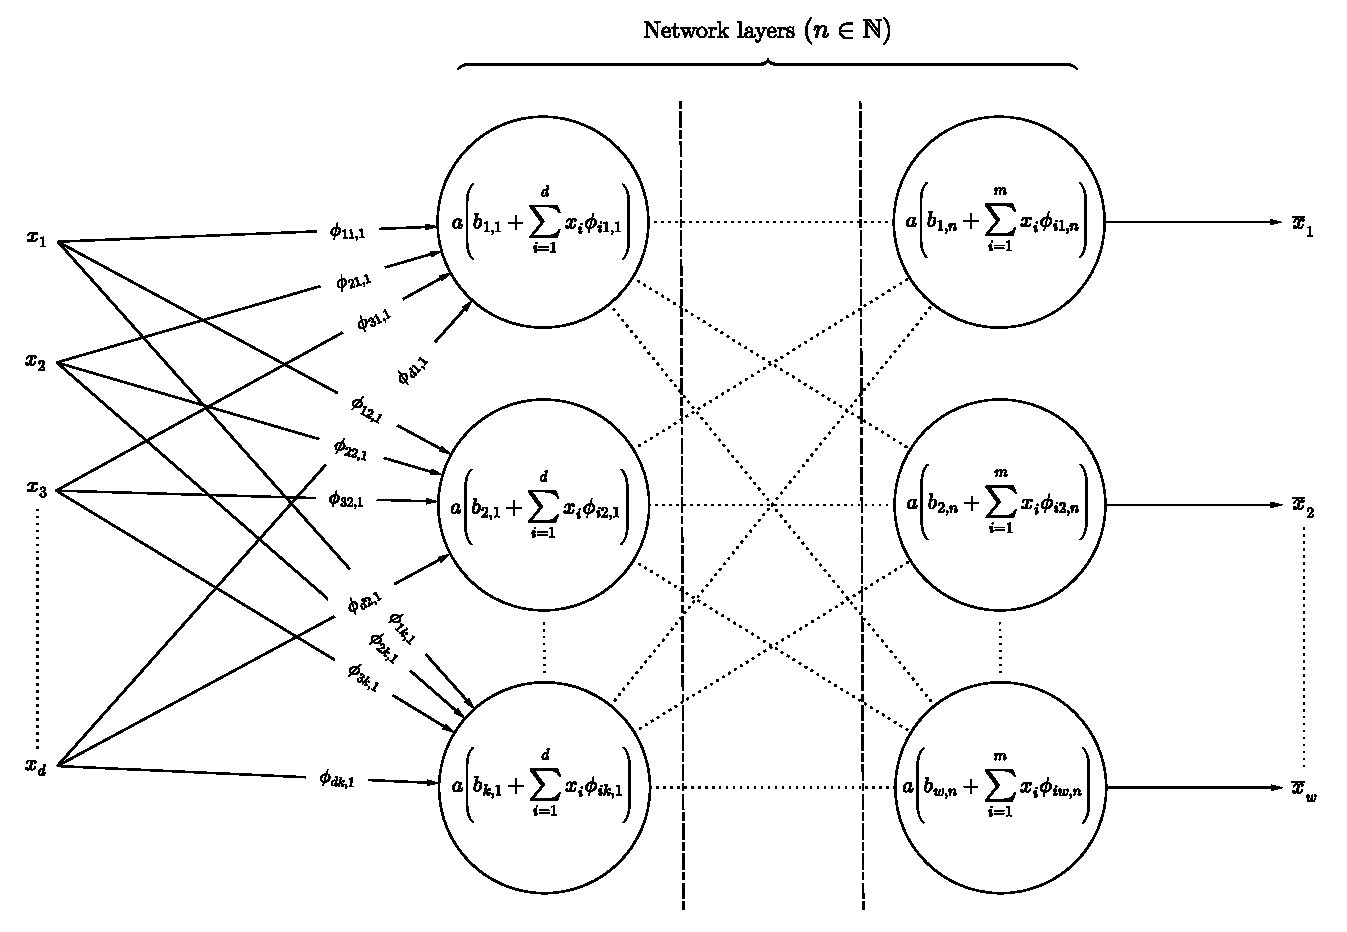
\includegraphics[width=\textwidth]{figures/MLP.pdf}
\caption{Working principle of a multi layer perceptron; hereby, $a$ represents a nonlinear activation function $a :\mathbb{R}\rightarrow \mathbb{R},\, s\mapsto a(s)$.}
\label{fig:MLP}
\end{figure}
Again, all quantities with letters $b$ or $\phi$ compose the total weights vector $\vect{\phi}$ of the multi layer perceptron, which is the simplest possible neural network involving more than one perceptron.

\subsection{Training process for neural networks}\label{sec:training}
In order for a neural network to learn anything, it has to be conditioned by data, whose interpretation is known. This process is generally referred to as training of a neural network and requires a mathematical framework that allows for optimization. \fc{During the training process of a neural network, one would like to achieve the best possible performance of the neural network in interpreting the training data correctly, that is to say, that the input data maps to known output data with minimal discrepancies.}

The mathematical framework for such an optimization relies on the definition of a loss function $\mathcal{L}_{\vect{\phi}}$, \fc{which is to be minimized by a suitable algorithm.} \fc{Let now $\{\tilde{\vect{x}}_1,\dots,\tilde{\vect{x}}_m\}$ be a set of known input data with a corresponding set $\{\hat{\vect{x}}_1,\dots,\hat{\vect{x}}_m\}$ of known output data, thus constituting the two training data matrices $\tilde{\matr{x}}$ and $\hat{\matr{x}}$. Let furthermore \begin{equation}
\vect{f}_{\vect{\phi}(\tilde{\matr{x}},\hat{\matr{x}})}: \mathbb{R}^d \rightarrow \mathbb{R}^w
\end{equation} represent a neural network as sketched in \cref{fig:MLP}, whereby $\vect{\phi}$ denote its weights and biases depending themselves on the training data $\tilde{\matr{x}}$ and $\hat{\matr{x}}$. The neural network $\vect{f}_{\vect{\phi}(\tilde{\matr{x}},\hat{\matr{x}})}$ then has the task of learning to correctly map an element $\tilde{\vect{x}}_i$ of the known input data to the corresponding element $\hat{\vect{x}}_i$ of the known output data. A loss function appropriately capturing this requirement can then be implemented in many different ways; for example, \lk{one} can just take the sum of norms of the differences between the generated outputs $\vect{f}_{\vect{\phi}(\tilde{\matr{x}},\hat{\matr{x}})}(\tilde{\vect{x}}_j)$ and the known outputs $\hat{\vect{x}}_j$, i.e. $\mathcal{L}_{\vect{\phi}(\tilde{\matr{x}},\hat{\matr{x}})} = \sum_{j=1}^{m}\|\hat{\vect{x}}_j-\vect{f}_{\vect{\phi}(\tilde{\matr{x}},\hat{\matr{x}})}(\tilde{\vect{x}}_j)\|$.} However, the \fc{optimal choice of} loss function depends on the task at hand and needs to be chosen accordingly, such that it represents a suitable measure on how well a neural network learns from the training data. Once one has defined a loss function $\mathcal{L}_{\vect{\phi}}$, the key to training a neural network resides within something called gradient descent. The idea behind gradient descent is quite simple; one just calculates the gradient of the loss function $\mathcal{L}_{\vect{\phi}}$ with respect to the weights $\vect{\phi}$, i.e. $\vect{\nabla}_{\vect{\phi}}\mathcal{L}_{\vect{\phi}}$ and updates all weights such that one moves into the direction of negative gradient. Iteratively repeating this process, eventually a local or global minimum of the loss function is found. In terms of mathematics, this procedure translates as follows. Consider some starting point $\vect{\phi}_i$ and the loss function at this point, i.e. $\mathcal{L}_{\vect{\phi}_i}$. The gradient $\vect{\nabla}\mathcal{L}_{\vect{\phi}}$ of the loss function with respect to the weights $\vect{\phi}$ indicates, in which direction of $\vect{\phi}$ the loss function increases or decreases. The negative gradient points into the direction of a local/global minimum of $\mathcal{L}_{\vect{\phi}}$, whereas the positive gradient points towards a local/global maximum. Hence, $\vect{\phi}_{i+1} = \vect{\phi}_{i} - \gamma \vect{\nabla}_{\vect{\phi}}\mathcal{L}_{\vect{\phi}_i}$ with $i \in \mathbb{N}$ and $\gamma > 0$ a suitable step size provides a rule for eventually finding a global or local minimum of the loss function. 
\begin{figure}[h]
\centering
\includegraphics[width=7cm]{figures/gradientdescent.pdf}
\caption{Visualization of a gradient descent routine. Note, that the horizontal axis is in reality multidimensional, whereas it is pictured here as just being one-dimensional. The vertical axis represents the value of the loss function $\mathcal{L}_{\vect{\phi}}$ in dependence of the weights $\vect{\phi}$.}
\label{fig:gradientdescent}
\end{figure}
One can therefore define an iterative procedure as follows:
\begin{enumerate}
\item Take a start value $\vect{\phi}_0$ and calculate the value of the loss function $\mathcal{L}_{\vect{\phi}_0}$ at this point.
\item Update the weights $\vect{\phi}_{i}$ according to the rule \begin{equation}
\vect{\phi}_{i+1} = \vect{\phi}_{i} - \gamma \vect{\nabla}_{\vect{\phi}}\mathcal{L}_{\vect{\phi}_i}
\end{equation} for $i \in \mathbb{N}$ individual steps and a suitable step size $\gamma > 0$ as long as $\epsilon \leq |\mathcal{L}_{\vect{\phi}_{i+1}}-\mathcal{L}_{\vect{\phi}_{i}}|$ holds for an accuracy threshold $\epsilon > 0$.
\item Terminate, if $\epsilon > |\mathcal{L}_{\vect{\phi}_{i+1}}-\mathcal{L}_{\vect{\phi}_{i}}|$.
\end{enumerate}
This iterative process is found visualized in \cref{fig:gradientdescent}; note, that this is a simplified picture, as the horizontal axis would in reality be multidimensional.

\subsection{Learning curves}\label{sec:learningcurves}
It is the goal of any entity of machine learning to learn from data in such a way, that it enables the machine learning entity to make as accurate as possible predictions on prior unseen data. \cite[p.110]{Goodfellow.2016} speak in this context of generalization, by which they mean the ability of a machine learning model to perform well on previously unobserved data. In order for a machine learning model to do that, it has to learn model parameters and mathematical operations to predict an outcome, given some input. It is crucial to a good performance of a machine learning model on prior unseen data, that the model learns those parameters and mathematical operations such that there is neither overfitting or underfitting of the model, \lk{nor underrepresentation present in the training and testing data.}

Overfitting is the case, where a model has learned too many parameters, such that it performs extremely well on the training data, but increasingly bad on testing data - that is to say, on prior unseen data to the model. The contrary - underfitting - means, that a model has not learned enough parameters to be able to generalize to prior unseen data.

Apart from overfitting, underfitting or underrepresentation issues, one can certainly ask if it matters, which particular model \lk{ansatz} one chooses for a particular task. In fact, \cite[p.116]{Goodfellow.2016} note that the so-called no free lunch theorem states, that every machine learning classification algorithm generalizes equally well (or bad), if averaged over all possible data generating probability distributions. But this is not to say, that every machine learning algorithm performs equally well or bad on a particular task - this is not the case. Hence, one must choose the most appropriate machine learning model for the task at hand. Most appropriate in this context is to say, that the chosen model should generalize better than any other available model ansatz \lk{for the chosen task.}

Once one has selected a machine learning model for a particular task, the question \lk{arises} of how to ensure that the model is trained on data in such a way, that it generalizes best to prior unobserved data. Methods to take care of this are generally known under the term ``regularization'', as \cite[p.120]{Goodfellow.2016} explain.

However, besides regularization, tuning the so-called hyperparameters of a machine learning algorithm can improve its generalization properties. Hyperparameters are just settings of the learning algorithm for a machine learning entity. \lk{In order to find optimal hyperparameters, either so-called grid search algorithms can be applied; or one can just inspect the learning curves for different settings of hyperparameters.} \fc{In the ideal case, both procedures are carried out, since the learning curves themselves do not provide enough information as to determine, which hyperparameters are optimal for a certain model.}
\begin{figure}[h]
\centering
\includegraphics[width=\textwidth]{figures/learningcurves.pdf}
\cprotect\caption{Examples for the four basic cases of non-ideal model performance. Sketches inspired by Jason Brownlee, \url{https://machinelearningmastery.com/learning-curves-for-diagnosing-machine-learning-model-performance/}, accessed on December 18, 2023.}
\label{fig:learningcurves}
\end{figure}

The concepts of underfitting, overfitting or underrepresentation of either training or testing data for the learning process of a machine learning model reflect in the learning curves as sketched in \cref{fig:learningcurves}. 

\lk{As underfitting means that the model has not learned enough parameters to generalize to unseen data,} it reflects in a learning curve such that the train loss is notoriously lower than the test loss and that there is an approximately constant gap between the train and test loss curves after several epochs. This situation is shown on the far left panel of \cref{fig:learningcurves}. 

If however the test loss steadily increases as the train loss continuously decreases, it is very likely that there is overfitting in the model; that is to say, that the model has learned too many model parameters, such that it performs very well on the training data, but increasingly worse on the test data. The situation of overfitting is shown in the second from left panel of \cref{fig:learningcurves}. 

Furthermore, there can also be two cases of underrepresentativeness of either the training dataset or the testing dataset, both of which are visualized in the two panels to the right in \cref{fig:learningcurves}. If the training dataset is not representative of the testing dataset and hence generally \lk{of} prior unseen data, one would expect that the test loss is higher than the train loss. This is indeed the case for an underrepresentative training dataset; additionally, there can be large fluctuations in the learning curves, since the gradient descent algorithm tends to jump over local or global minima of the loss function more easily, if the training data has ``gaps''. On the other hand, if the testing dataset is underrepresentative, one would expect that the test loss is notoriously lower than the train loss - because the average performance of a model trained on a diverse and therefore representative amount of data on a smaller, underrepresentative dataset will be better. That again is the case as shown in the far right panel of \cref{fig:learningcurves}, where once more fluctuations are to be expected due to the mentioned reason. 

Another factor that can lead to a behaviour a\fc{s} shown in the second to right panel of \cref{fig:learningcurves} is a learning rate, which is chosen to be too high. If the learning rate is \fc{set too large}, the gradient descent process optimizing the model parameters can ``jump'' over minima, leading to an oscillatory behaviour of the train and test losses.

An ideal learning curve is shown in \cref{fig:ideallearningcurve}.
\begin{figure}[h]
\centering
\includegraphics[width=6cm]{figures/ideallearningcurve.pdf}
\caption{Example of an ideal learning curve.}
\label{fig:ideallearningcurve}
\end{figure}
It features a continuously decreasing train and test loss, which eventually seem to converge to a constant value after several epochs and where furthermore the gap between the train and test losses is very small. An ideal learning curve indicates, that the hyperparameter setting for a machine learning model is optimal or at least well-chosen.

Analyzing learning curves visually using these tools can lead to finding optimal hyperparameters for machine learning model\lk{s} and especially for neural networks. Inspecting learning curves can also help to identify possible issues concerning the data itself, for example if the \lk{training or testing} data is underrepresentative of the general diversity of data or not.

\section{Deep generative models}
If not otherwise mentioned, the following treatment of deep generative models is based on the content given in \cite{weng2018flow}. Generative models - as their name already suggests - generate data. These models learn how to do so by extracting defining features of the data they are trained on, such as the data's probability density. Consider a matrix of training data $\hat{\matr{x}}$, where the individual columns follow a probability distribution $\vect{x} \sim p_{\vect{x}}(\vect{x})$. According to \cite[p.593]{Raschka.2022}, a generative model in deep learning is then defined such, that it learns parameters $\vect{\phi}(\hat{\matr{x}})$ to construct a probability density function $p_{\vect{\phi}(\hat{\matr{x}})}(\vect{x}) \approx p_{\vect{x}}(\vect{x})$. This is to say, that one can then draw samples from the learned probability density $p_{\vect{\phi}(\hat{\matr{x}})}(\vect{x})$, which essentially are generated data imitating the training data.

One can distinguish at least three basic architectures of generative models, namely variational autoencoder networks (VAE's), generative adversarial networks (GAN's) and flows. These types of generative models are visualized in \cref{fig:VAE}, \cref{fig:GAN} and \cref{fig:Flow}. The parallelograms used to visualize the working principles of these models represent dimensionality reduction/increase of an input variable compared to an output variable; if the parallelogram narrows towards the output, it means dimensionality reduction, whereas if it broadens towards the output, increase in dimensionality is visualized.
%Explain why in the context of inversions a flow is desirable (probability distribution for solution, rather than one single value, fast sampling due to essentially just a function, etc.). See blog of Lilian Weng.
\subsection{VAE's}
Variational autoencoders work as sketched in \cref{fig:VAE}. A variational autoencoder consists of an encoder and a decoder. The encoder implements a conditional probability distribution $q_{\vect{\phi}}(\vect{z}|\vect{x})$ for a latent variable $\vect{z}$, based on an input variable $\vect{x}$, where $\vect{\phi}$ are the weights of the neural network constituting the encoder. The decoder however models the probability $p_{\vect{\theta}}(\vect{x}|\vect{z})$ of the output variable $\vect{x}$ based on the latent variable $\vect{z}$, where again $\vect{\theta}$ are weights associated to the neural network of the decoder. The variable $\vect{x}$ represents the input variable with probability density $\vect{x} \sim p_{\vect{x}}(\vect{x})$, whereas the variable $\vect{z}$ is a latent variable and is chosen to fit the probability density of a standard normal distribution, i.e. $\vect{z}\sim p_{\vect{z}}(\vect{z}) = \mathcal{N}(0,1)^d$, where $d \in \mathbb{N}$ is the dimension of the latent variable.
\begin{figure}[h!]
\centering
\includegraphics[width=\linewidth-4cm]{figures/VAE.pdf}
\caption{Working principle of a variational autoencoder (VAE). Figure inspired by \cite{weng2018flow}.}
\label{fig:VAE}
\end{figure}

A variational autoencoder is trained in such a way, that the encoder learns how to transform an input $\vect{x}$ such that the output $\bar{\vect{z}}$ follows the chosen latent probability density. Furthermore, the decoder has to learn, how to transform a variable $\vect{z}$ following a standard normal distribution to an output $\bar{\vect{x}}$, such that the output variable follows the probability density of the original input variable $\vect{x}$.

A VAE in principle can be said to learn the most important information from the training data $\hat{\matr{x}}$, as it has to pass this information from the input variable $\vect{x}$ through a low-dimensional bottleneck to $\bar{\vect{z}}$, from which again the original input $\bar{\vect{x}}$ has to be reconstructed as best as possible, such that $\vect{x} \approx \bar{\vect{x}}$. Once the VAE is trained sufficiently, one can just use the decoder to generate outputs $\bar{\vect{x}}$ based on vectors $\vect{z}$ sampled from a multidimensional standard normal distribution.

A VAE could be used for stellar atmosphere inversion purposes, but it has several disadvantages in this regard compared to normalizing flows. First of all, VAE's have to be trained using an evidence lower bound (ELBO), because the exact likelihood of $\vect{x}$ given $\vect{z}$ is not tractable. A normalizing flow however allows for exact likelihood estimation of $\vect{x}$ given $\vect{z}$ because of its architecture. Furthermore, again because of its inherent architecture, a normalizing flow allows to perform exact inversions of data, since it is basically built of invertible functions. This is not the case for VAE's; yes, encoder and decoder are sort of inverse to one another, but it cannot be an exact inversion in the mathematical sense, since the VAE relies on \lk{dimensionality reduction}.

\subsection{GAN's}
% Explain what happens with a GAN.
Generative adversarial networks function as sketched in \cref{fig:GAN}. A generative adversarial network consists of a generator and a discriminator. The generator is \fc{basically a} function $\bar{\vect{x}} = \vect{G}_{\vect{\phi}}(\vect{z})$, where $\bar{\vect{x}}$ is the output of the generator, $\vect{\phi}$ are the weights associated to the neural network implementing the generator function and $\vect{z}$ is a latent variable, which is chosen to follow a standard normal distribution, i.e. $\vect{z} \sim p_{\vect{z}}(\vect{z}) = \mathcal{N}(0,1)^d$ with $d \in \mathbb{N}$ again the dimensionality of the latent space. The purpose of the generator is to generate fake data $\bar{\vect{x}}$ based on samples $\vect{z}$ of the latent probability density $p_{\vect{z}}(\vect{z})$. The discriminator however takes an input $\vect{x}$, such as the output of the generator, and outputs a value 0 or 1, where 0 stands for ``input is fake'' and 1 represents the situation ``input is real''. The task of the discriminator is therefore to decide, if an input $\vect{x}$ is fake or real.
\begin{figure}[h!]
\centering
\includegraphics[width=\linewidth-4cm]{figures/GAN.pdf}
\caption{Working principle of a generative adversarial network (GAN). Figure inspired by \cite{weng2018flow}.}
\label{fig:GAN}
\end{figure}

A generative adversarial network is trained in such a way, that the generator learns how to generate the best possible real-looking data $\bar{\vect{x}}$, whereas the discriminator learns as good as possible to distinguish between real data contained in the training set $\hat{\matr{x}}$ and fake data $\bar{\vect{x}}$ generated by the generator. Herein lies the adversarity of the model; the generator and the discriminator are actually competing against each other; the generator learns how to create the best possible fake data, whereas the discriminator learns, how to best distinguish between real and fake data - in this way, both the generator and the discriminator are optimized for their respective task. The loss function for training therefore has to be defined accordingly in a game-theoretical manner, where both the discriminator and the generator try to optimize their outcomes. Once trained, one can just use the generator to create fake data $\bar{\vect{x}} = \vect{G}_{\vect{\phi}}(\vect{z})$ from samples $\vect{z}$ of $p_{\vect{z}}(\vect{z})$ at will.

Despite the many interesting applications of GAN's, \fc{it is very challenging to use them for stellar atmosphere inversion purposes, since they do not suit the problem at hand.}

\subsection{Flows}
Flow-based generative models work as sketched in \cref{fig:Flow}. A flow just consists of a bijective function $\bar{\vect{z}} = \vect{f}_{\vect{\phi}}(\vect{x})$, where $\vect{\phi}$ refers to the weights of the neural network(s) used to implement this function. One of the main differences between flows and GAN's on the one hand and VAE's on the other hand is the fact, that flows are bijective in architectural nature, while GAN's and VAE's are not. This is to say that they are perfectly adapted to an inversion problem, such as a stellar atmosphere inversion task. Because of the bijective nature of flows, there is no dimensionality reduction or increase from input/output to latent space.
\begin{figure}[h!]
\centering
\includegraphics[width=\linewidth-4cm]{figures/Flow.pdf}
\caption{Working principle of a flow-based generative model. Figure inspired by \cite{weng2018flow}.}
\label{fig:Flow}
\end{figure}

Flows can be trained by exact likelihood calculation; that is to say, the loss function can be mathematically derived and implemented using the change of variable theorem from probability calculus in combination with the specific bijective transformations constituting the flow. A flow is called a normalizing flow, if the latent probability density function is chosen as a standard normal distribution - hence an arbitrary probability density $p_{\vect{x}}(\vect{x})$ of input data is mapped into the density of a standard normal distribution. In that way, the input data can be said to be normalized to the latent space. As flows and especially normalizing flows are best suited to stellar atmosphere inversions compared to the other available generative models, this technique will be the tool of choice in the material to follow.

%\section{Role of CPU's and GPU's in machine learning tasks}
%So-called CPU's (central processing unit) are those hardware components in a computer, which executes most of the computer's hardware and software instructions. CPU's performs tasks sequentially; therefore a CPU can only handle multiple tasks at the same time if there are multiple cores in the CPU.
%
%So-called GPU's (graphics processing unit) are those hardware components in a computer, which render intensive high-resolution graphics or images. GPU's can perform tasks in parallel processing; therefore a GPU can handle multiple tasks at the same time by splitting up a task in multiple sub-tasks and dividing them among the vast number of processing cores in the GPU.
%
%A CPU typically operates much faster than a GPU, but can handle tasks only sequentially. A GPU however typically consists of a vast number of cores allowing for efficient multitasking. In general therefore, a GPU can handle intensive calculations faster than a CPU, because it allows for dividing a task in multiple sub-tasks and distributing them among the vast number of processing cores, whereas the CPU cannot do that but can only handle tasks in a sequential way.
%
%For machine learning therefore, it is often the case that a GPU's are required for time-efficient computing.


%\section{Kullback-Leibler divergence}
%The Kullback-Leibler divergence is a means to compute how different two probability distributions $p(x)$ and $q(x)$ over the same random variable $X$ are. It is defined as \begin{equation}
%D_{KL}(p||q) = E_{x\sim p}\left[\log\left(\frac{p(x)}{q(x)}\right)\right] = E_{x\sim p}\left(\log[p(x)]-\log[q(x)]\right).
%\end{equation} As such, the Kullback-Leibler divergence is nothing more than the difference between a so-called cross-entropy $H_p[q(x)]$ and an entropy $H_p[q(x)]$, namely \begin{gather}\begin{gathered}
%D_{KL}(p||q) = H_p[q(x)]- H_p(p(x)) = -E_{x\sim p}(\log[q(x)]) + E_{x\sim p}(\log[p(x)]) \\ = E_{x\sim p}(\log[p(x)]- \log[q(x)]).
%\end{gathered}\end{gather} The Kullback-Leibler divergence will be low, if $p(x)$ and $q(x)$ are very similar; it will be high, if $p(x)$ and $q(x)$ are very different. 
%
%As information entropy is a measure for uncertainty in a probability distribution, divergence is to be interpreted as additional uncertainty accounting for the distance between two probability distributions over the same random variable. If $p(x)$ is the target probability distribution, i.e. the true distribution for the random variable $X$, and if $q(x)$ is the model probability distribution, i.e. the learned distribution, the Kullback-Leibler divergence provides a measure on how close the model probability distribution $q(x)$ is to the target distribution $p(x)$. Minimizing the Kullback-Leibler divergence is equivalent to finding the best model probability distribution $q(x)$ in terms of optimal resemblance to the target distribution $p(x)$.
\FloatBarrier

\section{Introduction to normalizing flows}
Normalizing flows are useful to learn complex data distributions from available samples, be they experimentally obtained or of a synthesized nature. 

The goal of a normalizing flow is to learn a certain probability density function $p_{\vect{x}}(\vect{x})$ of some quantity represented by a potentially multivariate random variable $\vect{x}$. Given samples from $p_{\vect{x}}(\vect{x})$ obtained by either experimental or synthetical procedure, the normalizing flow can learn the probability density function by means of finding a diffeomorphism, which maps samples $\vect{z}$ from a standard normal distribution to $p_{\vect{x}}(\vect{x})$. Since a diffeomorphism is invertible by definition, a trained normalizing flow can then be used to draw samples from the normalizing-flow-approximation of $p_{\vect{x}}(\vect{x})$ at will; this can be done by sampling from a standard normal distribution and subsequent application of the inverse learned diffeomorphism to the generated samples.

This technique can be used for various purposes; for example, for inversion problems in (stellar) atmospheric physics, as it is being explored in the subsequent material.

%The paper ``Bayesian Stokes inversion with normalizing flows'' by Diaz Baso et al. explores the possibility of a normalizing flow applied to learn how to do an inversion of a stellar atmosphere. 
%
%The paper is concerned with a classical inversion problem concerning stellar atmospheres. That is to say, that one would like to infer possible values for parameters of a solar model depending on measurement data. The paper elaborates on a method, called the Bayesian Stokes inversion with normalizing flows, in order to infer a parameter space of a stellar atmosphere model based on observations. What is special about this method is the fact, that not only certain solution values for the model parameters, but a whole distribution of possible solution values for these parameters are obtained.

\subsection{Why use normalizing flows for inversions?}
If one has an analytical model $\vect{y} = \vect{M}(\vect{x})$ of a stellar atmosphere, it can in some cases be analytically inverted, such that one has $\vect{x} = \vect{M}^{-1}(\vect{y})$. This raises the question, why one should even bother using normalizing flows to learn such inversions.

First of all, only simple models of radiative transfer such as the Milne-Eddington atmosphere can be inverted analytically. \lk{More complex models require resource-demanding numerical calculations to do inversions.} The advantage of a normalizing flow resides in the fact, that inversions done by it would be comparatively much faster, once the normalizing flow is trained.

A second incentive to use normalizing flow for atmospheric inversions is, that a normalizing flow not only provides one with one solution to the inversion problem for each atmospheric parameter, but rather with a probability density for each parameter. This allows for error estimation and the determination of the most likely solution to an inversion problem, if there is more than one solution possible.

\lk{\subsection{State of the art summary: Normalizing flows applied to inversions of stellar atmospheres}}
\lk{The normalizing flow technique in machine learning is to be considered as a relatively recent development. \cite{Rezende.21.05.2015} introduced normalizing flows in 2015 as a new and innovative solution to approximate posterior probability densities in variational inference. According to \cite[p.2]{Blei.2017}, variational inference refers to a class of machine learning techniques dedicated to finding complex posterior probability density functions by means of an optimization problem. Writing it in terms of Bayesian statistics, it is the study of how to calculate an approximation for the posterior density function $p(\vect{x}|\vect{y})$ given by the Bayes theorem as
\begin{equation}
p(\vect{x}|\vect{y}) = \frac{p(\vect{y}|\vect{x})p(\vect{x})}{\int_{\mathbb{R}^d} p(\vect{y}|\vect{x})p(\vect{x})\,\mathrm{d}\vect{x}},
\end{equation} if it is challenging to calculate this posterior density directly. Hereby, $\vect{x}$ are model parameters of a model $\vect{y} = \vect{M}(\vect{x})$, where $\vect{y}$ are identified as observations to be explained by the model and the model parameters. As a conclusion of their work, \cite[p.8]{Rezende.21.05.2015} point out that normalizing flows allow for the construction of extremely rich posterior density functions; having tested normalizing flows on different kinds of non-Gaussian 2D distributions of data and also the MNIST\footnote{See \cite{lecun-gradientbased-learning-applied-1998} for an extensive discussion on the MNIST dataset.} dataset. The MNIST dataset basically just consists of 70000 28 x 28 pixel images of labeled handwritten digits, 10000 of which pertain to the test dataset and the other 60000 to the train dataset.}

\lk{An effort to apply normalizing flows as a generative model for images was made by \cite{Dinh.27.05.2016}. They demonstrated, that normalizing flows can successfully be trained on datasets of images to generate similar images as the normalizing flow was trained on. In their work , they used the affine coupling layer type normalizing flow\footnote{This type of normalizing flow architecture is elucidated in \cref{subsec:normflowsaffinecouplinglayers}.}, which proved its applicability to image generation.}

\lk{Furthermore, \cite{Durkan.10.06.2019} showed that normalizing flows using the piecewise quadratic rational spline coupling layer architecture\footnote{This type of architecture is explained in \cref{subsec:normflowspiecewiserational}.} prove to be extremely powerful in density estimation for posterior densities and generative modeling of images.}

\lk{In terms of applications of normalizing flows to inversions of solar observations, to the best knowledge of the author there seems to be only one paper to this day, namely the paper on Bayesian Stokes inversion with normalizing flows by \cite{DiazBaso.2022}. In their paper, they explore the applicability of normalizing flows to learn inversion tasks of the solar atmosphere and illustrate, that if the normalizing flow transformations are conditioned on observations, it can be trained to return a posterior probability density estimate for any observation, i.e. the probability density $\vect{x} \sim p_{\vect{\phi}(\hat{\matr{x}},\hat{\matr{y}})}(\vect{x}|\vect{y})$ for any observation $\vect{y}$ of choice. Hereby, $\vect{\phi}(\hat{\matr{x}},\hat{\matr{y}})$ are the normalizing flow model parameters associated with the trained flow, which therefore depend on the training data $\hat{\matr{x}}$ and $\hat{\matr{y}}$. As \cite[p.11]{DiazBaso.2022} show, normalizing flows of the piecewise quadratic rational spline coupling layer type prove to serve as a reliable and fast tool to infer posterior parameter densities for photospheric and chromospheric spectral line observations in two cases; a local thermodynamic equilibrium (LTE) case (Milne-Eddington atmosphere) and a non-LTE case. They however did not consider observational data for the Stokes parameters $Q_\lambda$, $U_\lambda$ and $V_\lambda$ and hence left magnetic field properties of the target of interest out of consideration. As already suggested by \cite[p.11]{DiazBaso.2022} as a natural extension of their work, this is where the thesis at hand would like to fill a gap and expand the application of normalizing flows to the LTE case (Milne-Eddington atmosphere) taking into account all of the four Stokes parameters to infer magnetic field properties of the solar atmosphere.}

\section{Change of variable formula in probability theory}
The change of variable formula can be considered as the heart of the normalizing flow technique, since it guides the implementation of a loss function to train a flow. Because of its importance for normalizing flows, a full proof loosely following \cite[p.194-195]{Deisenroth.2020} of this theorem for the univariate case is given in \cref{sec:changeofvariableformula}; the formula itself is accounted for by \begin{equation}
	p_x(x) = p_z(f(x))\frac{\mathrm{d}f(x)}{\mathrm{d}x},
\end{equation} where $x$ and $z$ are continuous random variables with associated probability density functions $p_x(x)$ and $p_z(x)$. Furthermore, the random variable $z$ with the associated density function $p_z(z)$ denotes the transformed random variable $x$ by an invertible and smooth function $f(x)$, such that $z = f(x)$ and $x = f^{-1}(z)$ hold.
%will be given for the univariate case, which will be generalized to the multivariate case subsequently.

Let now $\vect{x}, \vect{z} \,\in\mathbb{R}^d,\,d\in\mathbb{N}$ be continuous multivariate random variables with associated probability density functions $p_{\vect{x}}(\vect{x})$ and $p_{\vect{z}}(\vect{z})$. \fc{In addition to this}, let 
\begin{equation} 
\vect{f}:\mathbb{R}^d \rightarrow \mathbb{R}^d, \quad \vect{x}\mapsto\vect{z} = \vect{f}(\vect{x}) 
\end{equation} be a diffeomorphism transforming $\vect{x}$ to $\vect{z}$. \cite[p.196]{Deisenroth.2020} in this case generalize the \lk{change of variable} formula \fc{from the univariate to} the multivariate case as \begin{align}\begin{aligned}
p_{\vect{x}}(\vect{x}) &= p_{\vect{z}}[\vect{f}(\vect{x})]\left|\det\left(\frac{\partial \vect{f}(\vect{x})}{\partial \vect{x}}\right)\right| \\ &= p_{\vect{z}}[\vect{f}(\vect{x})]\left|\det\begin{pmatrix}
\tfrac{\partial f_1(\vect{x})}{\partial x_1} & \dots & \tfrac{\partial f_1(\vect{x})}{\partial x_d} \\
\vdots & \ddots & \vdots \\
\tfrac{\partial f_d(\vect{x})}{\partial x_1} & \dots & \tfrac{\partial f_d(\vect{x})}{\partial x_d}
\end{pmatrix}\right|.
\end{aligned}\end{align}

\section{General principle of a normalizing flow}
% See Li Weng blog, just general theory without diving deep into

\subsection{Conceptual formulation of a normalizing flow}
Consider some vector $\vect{x} \in \mathbb{R}^d$ with $d,\,q \in \mathbb{N}$ and a latent vector $\vect{z} \in \mathbb{R}^d$. The probability densities for these vectors shall be given by \begin{equation}
\vect{x} \sim p_{\vect{x}}(\vect{x}), \quad \vect{z}\sim p_{\vect{z}}(\vect{z}) = \mathcal{N}(0,1)^d.
\end{equation}

The aim of a normalizing flow is to learn a diffeomorphism \begin{equation}
\vect{f}_{\vect{\phi}(\hat{\matr{x}})}:\mathbb{R}^d \rightarrow \mathbb{R}^d, \quad \vect{x} \mapsto \vect{z} = \vect{f}_{\vect{\phi}(\hat{\matr{x}})}(\vect{x})
\end{equation} transforming the probability density function $p_{\vect{x}}$ to $p_{\vect{z}}$. The conceptual principle of a normalizing flow is visualized in \cref{fig:normflow}. 
\begin{figure}[h]
\centering
\includegraphics[width=10cm]{figures/normflow.pdf}
\caption{Conceptual principle of a normalizing flow $\vect{z} = \vect{f}_{\vect{\phi}(\hat{\matr{x}})}(\vect{x})$ transforming a target probability density function $p_{\vect{x}}(\vect{x})$ to a base probability density function $p_{\vect{z}}(\vect{z})$.}
\label{fig:normflow}
\end{figure}
Hereby, $\vect{\phi}(\hat{\matr{x}})$ are weights depending on training data $\hat{\matr{x}} \in \mathbb{R}^{d\times q}$, which are associated to a deep neural network implementing the diffeomorphic function $\vect{f}_{\vect{\phi}(\hat{\matr{x}})}$. Given such a function, using the change of variable formula the probability density $p_{\vect{x}}(\vect{x})$ can be calculated as \begin{equation}
p_{\vect{x}}(\vect{x}) = p_{\vect{z}}[\vect{f}_{\vect{\phi}(\hat{\matr{x}})}(\vect{x})]\left|\det\left(\frac{\partial \vect{f}_{\vect{\phi}(\hat{\matr{x}})}(\vect{x})}{\partial \vect{x}}\right)\right|.
\end{equation} Knowing the transformation $\vect{z} = \vect{f}_{\vect{\phi}(\hat{\matr{x}})}(\vect{x})$ and given that $\vect{z} \sim \mathcal{N}(0,1)^d$, one can easily calculate samples from the normalizing-flow-approximation of the density $p_{\vect{x}}(\vect{x})$ by means of sampling $\vect{z}$ from a $d$-dimensional standard normal distribution and obtaining the corresponding $\vect{x}$ \lk{by} plugging $\vect{z}$ into the inverse function $\vect{f}_{\vect{\phi}(\hat{\matr{x}})}^{-1}$, such that $\vect{x} = \vect{f}_{\vect{\phi}(\hat{\matr{x}})}^{-1}(\vect{z})$ \lk{obtains}.

\subsection{Requirements for a normalizing flow}
Consider a function 
\begin{equation}
\vect{f}:\mathbb{R}^d \rightarrow \mathbb{R}^d, \quad \vect{x} \mapsto \vect{z} = \vect{f}(\vect{x})
\end{equation} composed of several functions $\vect{f}_{(k)}$, $k \in \{1,\dots,n\},\,n \in \mathbb{N}$, such that \begin{equation}
\vect{z} = \vect{f}(\vect{x}) = \vect{f}_{(n)} \circ \dots \circ \vect{f}_{(1)}(\vect{x}).
\end{equation} In this case, the transformation functions $\vect{f}_{(k)}$ aswell as the function $\vect{f}$ as a whole should satisfy several conditions to serve purposefully as a tool to sample from \lk{an approximation of} the probability density $p_{\vect{x}}(\vect{x})$ given samples $\vect{z}$ obtained from a standard normal distribution $p_{\vect{z}}(\vect{z})$. According to \cite{Kobyzev.2021}, all functions $\vect{f}_{(k)}$ should satisfy the following conditions:
\begin{enumerate}
\item All transformation functions $\vect{f}_{(k)}$ need to be invertible and differentiable. In order to transform one probability density into another density, it is necessary to calculate the Jacobian of the transformation function, as stated by the change of variable theorem. Furthermore, the transformation functions should be invertible, because one would like to sample from a standard normal distribution, plug the obtained values $\vect{z}$ into the inverse transformation function and thereby obtaining samples $\vect{x}$. Both of these conditions - invertibility and differentiabiliby - are satisfied by diffeomorphic functions.
\item The transformation functions $\vect{f}_{(k)}$ need to be expressive enough to model real data distributions. The normalizing flow composed of these transformation functions needs to learn a real data distribution; hence enough flexibility of the transformation functions is required in order to allow the neural networks composing the flow to learn actual and potentially complicated probability distributions.
\item The transformation functions $\vect{f}_{(k)}$ should be computationally efficient. That is, the Jacobian determinant should be calculable in an as efficient as possible way; furthermore also the application of the trained forward and inverse normalizing flow should consume as little as possible time. In order to train and apply the normalizing flow, i.e. the transformation functions composing the normalizing flow, many Jacobian determinants need to be calculated, as required by the change of variable formula. Therefore, transformation functions with a simple \lk{Jacobian} allowing for quick and easy calculations of the corresponding determinants are preferable.
\end{enumerate}

\subsection{Normalizing flows with conditioning data}
Consider a model $\vect{M}(\vect{x}) = \vect{y}$, that produces observations $\vect{y} \in \mathbb{R}^D,\,D \in \mathbb{N}$ based on model parameters $\vect{x}\in\mathbb{R}^d,\,d,\,q \in \mathbb{N}$. Furthermore, consider a latent vector $\vect{z} \in \mathbb{R}^d$. The probability densities for these vectors are given by \begin{equation}
\vect{x} \sim p_{\vect{x}}(\vect{x}), \quad \vect{y} \sim p_{\vect{y}}(\vect{y}), \quad \vect{z}\sim p_{\vect{z}}(\vect{z}) = \mathcal{N}(0,1)^d.
\end{equation}

The aim of the normalizing flow is to model the probability density $p_{\vect{\phi}(\hat{\matr{x}},\hat{\matr{y}})}(\vect{x}|\vect{y})$, namely the probability density function of $\vect{x}$, given a certain observation $\vect{y}$, thereby defining an inversion of the model $\vect{M}(\vect{x}) = \vect{y}$, see \cref{fig:normflowconditional} for a visualization of a normalizing flow with conditioning data. A normalizing flow modeling such a probability density will be called a conditional normalizing flow in the material to follow.
\begin{figure}[h]
\centering
\includegraphics[width=\textwidth]{figures/normflowconditional.pdf}
\caption{Conceptual principle of a conditional normalizing flow $\vect{z} = \vect{f}_{\vect{y},\vect{\phi}(\hat{\matr{x}},\hat{\matr{y}})}(\vect{x})$, transforming a target probability density function $p_{\vect{x}}(\vect{x})$ to a base probability density function $p_{\vect{z}}(\vect{z})$ \fc{conditioned} on $\vect{y} = \vect{M}(\vect{x})$, where $\vect{M}$ is a model that relates the data $\vect{x}$ to the conditioning data $\vect{y}$.}
\label{fig:normflowconditional}
\end{figure}
The multidimensional quantity $\vect{\phi}(\hat{\matr{x}},\hat{\matr{y}})$ is a set of parameters learned by a neural network, which is used to implement the normalizing flow.

If there is no conditioning data $\vect{y}$ available, the normalizing flow can directly be applied to learn the probability density $p_{\vect{\phi}(\hat{\matr{x}})}(\vect{x})$, \lk{which is essentially a normalizing-flow-approximation of the true probability density $p_{\vect{x}}(\vect{x})$.} In this case, the conditioning data $\vect{y}$, i.e. the symbols $\vect{y}$ and $\hat{\matr{y}}$, can be omitted in all formulae pertaining to the current chapter of this document.

\subsection{Coupling layer normalizing flows}\label{subsec:couplinglayernormalizingflows}
Consider a diffeomorphism \begin{equation}
\vect{f}_{\vect{y},\vect{\phi}(\hat{\matr{x}},\hat{\matr{y}})}: \mathbb{R}^d \rightarrow \mathbb{R}^d, \quad \vect{x} \mapsto \vect{z} = \vect{f}_{\vect{y},\vect{\phi}(\hat{\matr{x}},\hat{\matr{y}})}(\vect{x}),
\end{equation} where $\vect{\phi}(\hat{\matr{x}},\hat{\matr{y}})$ are weights depending on training data $\hat{\matr{x}} \in \mathbb{R}^{d\times q}$ and $\hat{\matr{y}} \in \mathbb{R}^{D \times q}$, which are associated to a deep neural network implementing the diffeomorphic function $\vect{f}_{\vect{y},\vect{\phi}(\hat{\matr{x}}, \hat{\matr{y}})}$. The probability density for $\vect{x}$ as calculated via $\vect{x}= \vect{f}^{-1}_{\vect{y},\vect{\phi}(\hat{\matr{x}},\hat{\matr{y}})}(\vect{z})$ therefore becomes conditional on the context $\vect{y}$, because the network parameters $\vect{\phi}(\hat{\matr{x}},\hat{\matr{y}})$ themselves depend on the context $\hat{\matr{y}}$ used to train the network. Hence for the normalizing-flow-approximation of $p_{\vect{x}}(\vect{x})$ conditioned on the data $\vect{y}$, the notation $p_{\vect{\phi}(\hat{\matr{x}},\hat{\matr{y}})}(\vect{x}|\vect{y})$ is introduced.

With the change of variable theorem, one obtains \begin{align}
\begin{aligned}
1 = \int_{\mathbb{R}^d} p_{\vect{z}}(\vect{z})\,\mathrm{d}\vect{z} &= \int_{\mathbb{R}^d}p_{\vect{z}}[\vect{f}_{\vect{y},\vect{\phi}(\hat{\matr{x}},\hat{\matr{y}})}(\vect{x})]\left|\det\left(\frac{\partial \vect{f}_{\vect{y},\vect{\phi}(\hat{\matr{x}},\hat{\matr{y}})}(\vect{x})}{\partial \vect{x}}\right)\right|\,\mathrm{d}\vect{x} \\ &= \int_{\mathbb{R}^d} p_{\vect{\phi}(\hat{\matr{x}},\hat{\matr{y}})}(\vect{x}|\vect{y})\,\mathrm{d}\vect{x},
\end{aligned}
\end{align} from which it follows, that the probability density $p_{\vect{\phi}(\hat{\matr{x}},\hat{\matr{y}})}(\vect{x}|\vect{y})$ can be expressed by means of the diffeomorphism $\vect{f}_{\vect{y},\vect{\phi}(\hat{\matr{x}},\hat{\matr{y}})}$, the Jacobian $\tfrac{\partial \vect{f}_{\vect{y},\vect{\phi}(\hat{\matr{x}},\hat{\matr{y}})}(\vect{x})}{\partial \vect{x}}$ and the probability density $p_{\vect{z}}(\vect{z})$, namely \begin{equation}\label{eq:heartofnormflowswithcontext}
p_{\vect{\phi}(\hat{\matr{x}},\hat{\matr{y}})}(\vect{x}|\vect{y}) = p_{\vect{z}}[\vect{f}_{\vect{y},\vect{\phi}(\hat{\matr{x}},\hat{\matr{y}})}(\vect{x})]\left|\det\left(\frac{\partial \vect{f}_{\vect{y},\vect{\phi}(\hat{\matr{x}},\hat{\matr{y}})}(\vect{x})}{\partial \vect{x}}\right)\right|.
\end{equation} This identity is to be considered as the key to implementing a loss function for the normalizing flow technique.

Since a concatenation of diffeomorphisms is again a diffeomorphism, the function $\vect{f}_{\vect{y},\vect{\phi}(\hat{\matr{x}},\hat{\matr{y}})}$ can be composed of many \lk{individual} diffeomorphisms. Let $\vect{f}_{\vect{y},\vect{\phi},(1)}, \dots, \vect{f}_{\vect{y},\vect{\phi},(n)}$ with $n \in \mathbb{N}$ be a number of diffeomorphisms, such that \begin{equation}
\vect{f}_{\vect{y},\vect{\phi}(\hat{\matr{x}},\hat{\matr{y}})} = \vect{f}_{\vect{y},\vect{\phi},(n)}\circ \dots \circ \vect{f}_{\vect{y},\vect{\phi},(1)}.
\end{equation} Introducing the notation $\vect{x} \doteq \vect{z}_{(0)}$, $\vect{z} \doteq \vect{z}_{(n)}$ and $\vect{z}_{(k)} \doteq \vect{f}_{\vect{y},\vect{\phi},(k)}(\vect{z}_{(k-1)})$ with $k \in \{1,\dots,n\}$, the function $\vect{f}_{\vect{y},\vect{\phi}(\hat{\matr{x}},\hat{\matr{y}})}$ can be written as \begin{equation}
\vect{f}_{\vect{y},\vect{\phi}(\hat{\matr{x}},\hat{\matr{y}})}(\vect{z}_{(0)}) = \vect{f}_{\vect{y},\vect{\phi},(n)}\circ \dots\circ \vect{f}_{\vect{y},\vect{\phi},(1)}(\vect{z}_{(0)}).
\end{equation} 
In \cref{fig:normflows}, an overview of the working principle of a coupling layer normalizing flow is visualized.
\begin{figure}[h!]
\centering
\includegraphics[width=\textwidth]{figures/normflows.pdf}
\caption{Visualization of the working principle of coupling layer normalizing flows.}
\label{fig:normflows}
\end{figure}
Because $\vect{f}_{\vect{y},\vect{\phi}(\hat{\matr{x}},\hat{\matr{y}})}(\vect{x})$ is a concatenation of functions $\vect{f}_{\vect{y},\vect{\phi},(k)}(\vect{z}_{(k-1)})$ with $k \in \{1,\dots,n\}$, the determinant of the Jacobian  for $\vect{f}_{\vect{y},\vect{\phi}(\hat{\matr{x}},\hat{\matr{y}})}(\vect{x})$ with respect to $\vect{x}$ is given by \begin{equation}
\det\left(\frac{\partial \vect{f}_{\vect{y},\vect{\phi}(\hat{\matr{x}},\hat{\matr{y}})}(\vect{x})}{\partial \vect{x}}\right) = \prod_{k=1}^{n}\det\left(\frac{\partial \vect{f}_{\vect{y},\vect{\phi},(k)}(\vect{z}_{(k-1)})}{\partial \vect{z}_{(k-1)}}\right),
\end{equation} where the Jacobians on the right-hand side take the form \begin{equation}
\frac{\partial \vect{f}_{\vect{y},\vect{\phi},(k)}(\vect{z}_{(k-1)})}{\partial \vect{z}_{(k-1)}} = 
\begin{pmatrix}
\frac{\partial f_{\vect{y},\vect{\phi},(k),1}(\vect{z}_{(k-1)})}{\partial z_{(k-1),1}} & \dots & \frac{\partial f_{\vect{y},\vect{\phi},(k),1}(\vect{z}_{(k-1)})}{\partial z_{(k-1),d}} \\
\vdots & \ddots & \vdots \\
\frac{\partial f_{\vect{y},\vect{\phi},(k),d}(\vect{z}_{(k-1)})}{\partial z_{(k-1),1}} & \dots & \frac{\partial f_{\vect{y},\vect{\phi},(k),d}(\vect{z}_{(k-1)})}{\partial z_{(k-1),d}}
\end{pmatrix}
\end{equation} with $k \in \{1,\dots,n\}$. 
Every function $\vect{f}_{\vect{y},\vect{\phi},(k)}(\vect{z}_{(k-1)})$ for $k \in \{1,\dots,n\}$ represents one of the $n$ so-called coupling layers constituting the total flow function $\vect{f}_{\vect{y},\vect{\phi}(\hat{\matr{x}},\hat{\matr{y}})}$. Every composite function $\vect{f}_{\vect{y},\vect{\phi},(k)}$ is implemented by application of neural networks depending on $\vect{x}$ and $\vect{y}$, such that each composite function is fully invertible and differentiable. The total set of parameters learned by the neural networks is then identified with $\vect{\phi}(\hat{\matr{x}},\hat{\matr{y}})$, hence defining the function $\vect{f}_{\vect{y},\vect{\phi}(\hat{\matr{x}},\hat{\matr{y}})}$.

\section{Affine coupling layer normalizing flow}\label{subsec:normflowsaffinecouplinglayers}
Affine coupling layer normalizing flows\cprotect\footnote{A basic implementation of an affine coupling layer normalizing flow in the \verb|PyTorch| framework is given by the author at \url{https://github.com/danielzahnd/master-thesis/tree/main/code/nf-affine-coupling-layer-normalizing-flow}.\label{footnote:NF_code}} are one of the most simple types of normalizing flows. They basically rely on a concatenation of many affine transformations, where the scale and shift parameters are implemented as neural networks. Although quite easy to implement, these type of flows lack flexibility, as noted by \cite[p.3]{Durkan.10.06.2019}. However, they provide good insight to the working principle of a normalizing flow and are sufficiently flexible for some less complex applications as shown in \cref{chap:proofofconcept}.
 
\subsection{Construction of an affine coupling layer normalizing flow}
The subsequent considerations about how to construct an affine coupling layer normalizing flow follow \cite[p.3-5]{Dinh.27.05.2016}. Consider a diffeomorphism \begin{align}\small \begin{aligned}
\vect{f}_{\vect{y},\vect{\phi}(\hat{\matr{x}},\hat{\matr{y}})} = \vect{f}_{\vect{y},\vect{\phi},(n)}\circ \dots \circ \vect{f}_{\vect{y},\vect{\phi},(1)}: \mathbb{R}^d \rightarrow \mathbb{R}^d, \quad \vect{x} \mapsto \vect{z} = \vect{f}_{\vect{y},\vect{\phi}(\hat{\matr{x}},\hat{\matr{y}})}(\vect{x}),
\end{aligned}\end{align} where all quantities are given as defined in \cref{subsec:couplinglayernormalizingflows}. 

In the case of $\vect{f}_{\vect{y},\vect{\phi},(k)}$ being so-called affine coupling layers, the functions can explicitly \fc{be} written by means of two arbitrary functions \begin{equation}
\vect{\mu}_{(k)}: \mathbb{R}^{m+D} \rightarrow \mathbb{R}^{d-m}, \quad \vect{\sigma}_{(k)}: \mathbb{R}^{m+D} \rightarrow \mathbb{R}^{d-m}
\end{equation} with $m \in \{1,\dots,d\}$ and $k \in \{1,\dots,n\}$ implemented as deep neural networks. That is to say, that the neural networks $\vect{\mu}_{(k)}$ and $\vect{\sigma}_{(k)}$ take a vector of dimension $m+D$ as an input and return a vector of dimension $d-m$ as an output; there can be an arbitrary sequence of network layers and activation functions in between input and output. Every mapping $\vect{z}_{(k)} = \vect{f}_{\vect{y},\vect{\phi},(k)}(\vect{z}_{(k-1)})$ for $k \in \{1,\dots,n\}$ is now defined as an affine transformation, such that \begin{align}
f_{\vect{y},\vect{\phi},(k),l}(\vect{z}_{(k-1)}) &= z_{(k-1),l}, \\
f_{\vect{y},\vect{\phi},(k-1),l}^{-1}(\vect{z}_{(k)}) &= 
z_{(k),l}
\end{align} for $l \in \{1,\dots,m\}$
and
\begin{align}
f_{\vect{y},\vect{\phi},(k),l}(\vect{z}_{(k-1)}) &= 
\mu_{(k),l}(\vect{z}_{(k-1),1:m},\vect{y}) + e^{\sigma_{(k),l}(\vect{z}_{(k-1),1:m},\vect{y})}\cdot z_{(k-1),l}, \\
f_{\vect{y},\vect{\phi},(k-1),l}^{-1}(\vect{z}_{(k)}) &= [z_{(k),l} - \mu_{(k),l}(\vect{z}_{(k),1:m},\vect{y})]\cdot  e^{-\sigma_{(k),l}(\vect{z}_{(k),1:m},\vect{y})}
\end{align} for $l \in \{m+1,\dots,d\}$, where $\vect{f}_{\vect{y},\vect{\phi},(k)} = (f_{\vect{y},\vect{\phi},(k),1},\dots,f_{\vect{y},\vect{\phi},(k),d})^\top$ and furthermore $\vect{z}_{(k),1:m} = (z_{(k),1},\dots, z_{(k),m})^\top$.

It is a convenient property of such affine functions $\vect{f}_{\vect{y},\vect{\phi},(k)}(\vect{z}_{(k-1)})$ for $k \in \{1,\dots,n\}$, that the Jacobians with respect to $\vect{z}_{(k-1)}$ are triangular, that is 
\begin{gather}\footnotesize\begin{gathered}
\frac{\partial \vect{f}_{\vect{y},\vect{\phi},(k)}(\vect{z}_{(k-1)})}{\partial \vect{z}_{(k-1)}} = 
\begin{pmatrix}
\mathds{1}_m & \mathds{O}_m \\
\frac{\partial \vect{f}_{\vect{y},\vect{\phi},(k),m+1:d}(\vect{z}_{(k-1)})}{\partial \vect{z}_{(k-1),m+1:d}} &  \mathrm{diag}\left(e^{\sigma_{(k),m+1:d}(\vect{z}_{(k-1),1:m},\vect{y})}\right)
\end{pmatrix},
\end{gathered}\end{gather} where $\mathds{1}_m$ is a unity matrix and $\mathds{O}_m$ is a zero matrix of dimension $m \times m$. The lower left quantity in the above matrix is again a Jacobian and takes the form \begin{gather}\scriptsize\begin{gathered}\label{eq:lowerleftjacobian}
\frac{\partial \vect{f}_{\vect{y},\vect{\phi},(k),m+1:d}(\vect{z}_{(k-1)})}{\partial \vect{z}_{(k-1),m+1:d}} = \begin{pmatrix}
\frac{\partial f_{\vect{y},\vect{\phi},(k),m+1}(\vect{z}_{(k-1)})}{\partial z_{(k-1),m+1}} & \dots & \frac{\partial f_{\vect{y},\vect{\phi},(k),m+1}(\vect{z}_{(k-1)})}{\partial z_{(k-1),d}} \\
\vdots & \ddots & \vdots \\
\frac{\partial f_{\vect{y},\vect{\phi},(k),d}(\vect{z}_{(k-1)})}{\partial z_{(k-1),m+1}} & \dots & \frac{\partial f_{\vect{y},\vect{\phi},(k),d}(\vect{z}_{(k-1)})}{\partial z_{(k-1),d}}
\end{pmatrix};
\end{gathered}\end{gather} the lower right quantity however is a diagonal matrix with the elements $e^{\sigma_{(k),l}(\vect{z}_{(k-1),1:m},\vect{y})}$ for $l \in \{m+1,d\}$ on the diagonal. Therefore, the Jacobian $\nicefrac{\partial \vect{f}_{\vect{y},\vect{\phi},(k)}(\vect{z}_{(k-1)})}{\partial \vect{z}_{(k-1)}}$ is triangular. \fc{According to a standard theorem from linear algebra as given by \cite[p.479]{Arens.2013}, the determinant of this expression is hence given} by the product of the diagonal elements, that is \begin{equation}\label{eq:determinantofdiagonalelements}
\det\left(\frac{\partial \vect{f}_{\vect{y},\vect{\phi},(k)}(\vect{z}_{(k-1)})}{\partial \vect{z}_{(k-1)}}\right) = \prod_{j = m+1}^{d}e^{\sigma_{(k),j}(\vect{z}_{(k-1),1:m},\vect{y})}.
\end{equation} \fc{Because of the triangularity of $\nicefrac{\partial \vect{f}_{\vect{y},\vect{\phi},(k)}(\vect{z}_{(k-1)})}{\partial \vect{z}_{(k-1)}}$, the lower left Jacobian \cref{eq:lowerleftjacobian} does not matter anymore for the determinant calculation.} Taking the logarithm of \fc{expression \cref{eq:determinantofdiagonalelements}} results in a transformation of the product to a sum, such that \begin{equation}\label{eq:previouslogdetc}
\log\left[\det\left(\frac{\partial \vect{f}_{\vect{y},\vect{\phi},(k)}(\vect{z}_{(k-1)})}{\partial \vect{z}_{(k-1)}}\right)\right] = \sum_{j = m+1}^{d}\sigma_{(k),j}(\vect{z}_{(k-1),1:m},\vect{y})
\end{equation} holds. Recall, that the complete normalizing flow is given as a concatenation of affine coupling functions (layers), such that \begin{gather}
\begin{gathered}
\det\left(\frac{\partial \vect{f}_{\vect{y},\vect{\phi}(\hat{\matr{x}},\hat{\matr{y}})}(\vect{x})}{\partial \vect{x}}\right) = \prod_{k = 1}^{n}\det\left(\frac{\partial \vect{f}_{\vect{y},\vect{\phi},(k)}(\vect{z}_{(k-1)})}{\partial \vect{z}_{(k-1)}}\right).
\end{gathered}
\end{gather} Taking the logarithm of this expression and inserting the previous result \cref{eq:previouslogdetc}, this  leads to \begin{align}\label{eq:finallogdetaffinecouplingc}
\begin{aligned}
\log\left[\det\left(\frac{\partial \vect{f}_{\vect{y},\vect{\phi}(\hat{\matr{x}},\hat{\matr{y}})}(\vect{x})}{\partial \vect{x}}\right)\right] &= \sum_{k = 1}^{n}\log\left[\det\left(\frac{\partial \vect{f}_{\vect{y},\vect{\phi},(k)}(\vect{z}_{(k-1)})}{\partial \vect{z}_{(k-1)}}\right)\right] \\
&= \sum_{k = 1}^{n}\sum_{j = m+1}^{d}\sigma_{(k),j}(\vect{z}_{(k-1),1:m},\vect{y}).
\end{aligned}
\end{align}

\fc{The general working principle of an affine coupling layer normalizing flow with just one coupling layer is visualized in \cref{fig:affinenormalizingflow_forward} and \cref{fig:affinenormalizingflow_backward}.}
\begin{figure}[h!]	
\centering
\includegraphics[width=\textwidth]{figures/affinenormalizingflow_forward.pdf}
\caption{Forward direction for a single-layer affine coupling layer normalizing flow.}
\label{fig:affinenormalizingflow_forward}
\end{figure}
\begin{figure}[h!]
\centering
\includegraphics[width=\textwidth]{figures/affinenormalizingflow_backward.pdf}
\caption{Backward direction for a single-layer affine coupling layer normalizing flow.}
\label{fig:affinenormalizingflow_backward}
\end{figure}

\subsection{Training process for affine coupling layer normalizing flows}
Recalling the diffeomorphism $\vect{z} = \vect{f}_{\vect{y},\vect{\phi}(\hat{\matr{x}},\hat{\matr{y}})}(\vect{x})$ and the change of variable formula for the multivariate case, the probability density $p_{\vect{\phi}(\hat{\matr{x}},\hat{\matr{y}})}(\vect{x}|\vect{y})$ can be written as found in \cref{eq:heartofnormflowswithcontext}. Taking the natural logarithm of expression \cref{eq:heartofnormflowswithcontext} and inserting the result \cref{eq:finallogdetaffinecouplingc} into it, one obtains
\begin{align}\begin{aligned}
\log\left[p_{\vect{\phi}(\hat{\matr{x}},\hat{\matr{y}})}(\vect{x}|\vect{y})\right] &= \log\left(p_{\vect{z}}[\vect{f}_{\vect{y},\vect{\phi}(\hat{\matr{x}},\hat{\matr{y}})}(\vect{x})]\right) \\ &\quad + \left|\sum_{k = 1}^{n}\sum_{j = m+1}^{d}\sigma_{(k),j}(\vect{z}_{(k-1),1:m},\vect{y})\right|.
\end{aligned}\end{align} Note, that the natural logarithm $\log(a)$ is strictly monotonic increasing for $a > 0$; furthermore, $-\infty < \log(a) \leq 0$ for $ 0 < a \leq 1$. Therefore, maximizing the so-called likelihood $p_{\vect{\phi}(\hat{\matr{x}},\hat{\matr{y}})}(\vect{x}|\vect{y})$ is equivalent to maximizing $\log\left[p_{\vect{\phi}(\hat{\matr{x}},\hat{\matr{y}})}(\vect{x}|\vect{y})\right]$, which is named the log-likelihood. Maximizing $p_{\vect{\phi}(\hat{\matr{x}},\hat{\matr{y}})}(\vect{x}|\vect{y})$ corresponds to finding optimal network parameters $\vect{\phi}(\hat{\matr{x}},\hat{\matr{y}})$ for the deep neural networks $\vect{\mu}_{(k)}$ and $\vect{\sigma}_{(k)}$ for $k \in\{1,\dots,n\}$ constituting the flow function $\vect{f}_{\vect{y},\vect{\phi}(\hat{\matr{x}},\hat{\matr{y}})}$, such that the most suitable model parameters $\vect{x}$ given some context $\vect{y}$ are found. In the case of a stellar atmosphere inversion, $p_{\vect{\phi}(\hat{\matr{x}},\hat{\matr{y}})}(\vect{x}|\vect{y})$ represents a probability distribution for the solutions $\vect{x}$ of an inversion $\vect{x} = \vect{M}^{-1}(\vect{y})$, where $\vect{M}$ is the atmosphere model and $\vect{y}$ are observations.

That is to say, that the normalizing flow, i.e. the neural networks constituting it, are trained by means of minimizing the negative log-likelihood $-\log\left[p_{\vect{\phi}(\hat{\matr{x}},\hat{\matr{y}})}(\vect{x}|\vect{y})\right]$, which is equivalent to maximizing positive log-likelihood and hence also to maximizing the positive likelihood. Therefore, the loss function to minimize by any algorithm employed can be defined as 
\begin{align}\footnotesize
\begin{aligned}
\mathcal{L}_{\vect{\phi}(\hat{\matr{x}},\hat{\matr{y}})}(\vect{x},\vect{y}) =&  -\log\left(p_{\vect{z}}[\vect{f}_{\vect{y},\vect{\phi}(\hat{\matr{x}},\hat{\matr{y}})}(\vect{x})]\right) - \log\left(\left|\det\left(\frac{\partial \vect{f}_{\vect{y},\vect{\phi}(\hat{\matr{x}},\hat{\matr{y}})}(\vect{x})}{\partial \vect{x}}\right)\right|\right) \\
=& -\log\left(p_{\vect{z}}[\vect{f}_{\vect{y},\vect{\phi}(\hat{\matr{x}},\hat{\matr{y}})}(\vect{x})]\right) - \left|\sum_{k = 1}^{n}\sum_{j = m+1}^{d}\sigma_{(k),j}(\vect{z}_{(k-1),1:m},\vect{y})\right|.
\end{aligned}
\end{align} This loss function is minimized with respect to the neural network parameters $\vect{\phi}(\hat{\matr{x}},\hat{\matr{y}})$.


%\section{Autoregressive normalizing flow}\label{subsec:normflowsautoregressive}
%\subsection{Conceptual formulation and terminology}
%Text.
%
%\subsection{Construction of an autoregressive normalizing flow}
%Text.
%
%\subsection{Training process for autoregressive normalizing flows}
%Text.

\section{Piecewise rational quadratic spline normalizing flow}\label{subsec:normflowspiecewiserational}
Affine coupling layer normalizing flows as \lk{described} in detail above are simple and relatively easy to implement, but they lack flexibility. These type of flows may especially struggle to model multimodal density functions using just affine transformations, as \cite[p.3]{Durkan.10.06.2019} remark. Recall, that as a base density usually a standard normal distribution is taken. If there are now multiple modes present in the target distribution of the data to model, the flow needs to learn how to transform just one mode present in the base distribution to the multiple modes in the multimodal target distribution, thus presenting the flow with the need to learn potentially highly nonlinear transformation\lk{s}. This is where affine coupling layer normalizing flows are at their limit. \lk{Since inversions of stellar atmospheres are especially prone to sometimes have more than one solution, a normalizing flow applied to learn stellar inversions needs to be able to model multimodal densities of the atmospheric parameters.} 
Hence, \cite[p.4]{Durkan.10.06.2019} introduce piecewise rational quadratic spline normalizing flows, which are more flexible in nature, but mathematically still relatively simple and furthermore fully invertible and differentiable, thus diffeomorphic. \fc{In \cref{fig:affinevsquadratic}, the advantage of piecewise quadratic spline normalizing flows over affine flows for modeling multimodal probability densities is visualized. Using piecewise quadratic functions, one can approximate a multimodal density $p_x(x)$ more accurately with the same amount of parameters as with affine functions.}
\begin{figure}[h!]
	\centering
	\includegraphics[width=\textwidth]{figures/affinevsquadratic.pdf}
	\caption{Approximating a probability density with affine or quadratic functions using the same amount of parameters in both cases. Both the affine and piecewise quadratic normalizing flow types essentially work by calculating optimal parameters of affine or quadratic functions, such that the probability density $p_x(x)$ is optimally approximated by ``pieces'' of those functions.}
	\label{fig:affinevsquadratic}
\end{figure}

\fc{The piecewise rational quadratic spline normalizing flow} type of normalizing flow is therefore the flow of choice for the more complex applications as presented and discussed in \cref{chap:results_and_discussion}. These kind of flows were however not implemented from scratch by the author, but the already existing software \cite{nflows} was made use of; and the theoretical considerations below follow the material as presented by \cite{Durkan.10.06.2019}.

\subsection{Construction of a piecewise rational quadratic spline normalizing flow}\label{sec:piecewisequadraticspline}
Consider a diffeomorphism \begin{align}\small\begin{aligned}
\vect{f}_{\vect{y},\vect{\phi}(\hat{\matr{x}},\hat{\matr{y}})} = \vect{f}_{\vect{y},\vect{\phi},(n)}\circ \dots \circ \vect{f}_{\vect{y},\vect{\phi},(1)}: \mathbb{R}^d \rightarrow \mathbb{R}^d, \quad \vect{x} \mapsto \vect{z} = \vect{f}_{\vect{y},\vect{\phi}(\hat{\matr{x}},\hat{\matr{y}})}(\vect{x}).
\end{aligned}\end{align} In the case of this function being implemented by piecewise rational quadratic spline coupling layers, these individual layers can be defined as follows.

Again, $\vect{x} \sim p_{\vect{x}}(\vect{x})$ and $\vect{y} \sim p_{\vect{y}}(\vect{y})$ hold, whereas the modelled probability density of $\vect{x}$ conditional on $\vect{y}$ as learned by a normalizing flow is denoted as $\vect{x} \sim p_{\vect{\phi}(\hat{\matr{x}},\hat{\matr{y}})}(\vect{x}|\vect{y})$, where $\vect{\phi}(\hat{\matr{x}},\hat{\matr{y}})$ are weights associated to the neural network(s) used to implement the flow. The quantities $\hat{\matr{x}} \in \mathbb{R}^{d\times q}$ and $\hat{\matr{y}} \in \mathbb{R}^{D \times q}$ once more represent the training data.

Consider an input vector $\vect{x} \in \mathbb{R}^d$ and a conditioning vector $\vect{y} \in \mathbb{R}^D$. Let now be a vector $\vect{s}$ defined, such that it contains the first $m$ entries of the input vector $\vect{x}$ and the whole conditioning vector $\vect{y}$, that is to say, $\vect{s} \doteq (x_1,\dots,x_m,y_1,\dots,y_D) \in \mathbb{R}^{m+D}$. In order to define a single layer $f_{\vect{y},\vect{\phi},(k)}$ with $k \in \{1,\dots,n\}$ of the flow, one requires $(d-m)(3K-1)$ parameters per layer $k$ These parameters are given for each layer $k$ by means of a neural network \begin{equation}
\vect{\mu}_{(k)}: \mathbb{R}^{m+D}\rightarrow \mathbb{R}^{(d-m)(3K-1)}, \quad \vect{s}_{(k-1)} \mapsto \vect{\mu}_{(k)}(\vect{s}_{(k-1)})
\end{equation} whereby $m \in \{1,\dots,d\}$, $k \in \{1,\dots,n\}$ and $K \in \mathbb{N}$. The integer $K$ is the number of spline knots of choice. The precise nature of the mapping $\vect{\mu}_{(k)}$ is that of an arbitrary neural network, which therefore cannot be explicitly written, but can be accounted for by
\begin{align}
\begin{aligned}
\vect{\mu}_{(k)}(\vect{s}_{(k-1)}) = \begin{pmatrix}
\mu_{(k),m+1,1}^w \\
\vdots \\
\mu_{(k),i,j}^w \\
\vdots \\
\mu_{(k),d,K}^w \\
\mu_{(k),m+1,1}^h \\
\vdots \\
\mu_{(k),i,j}^h \\
\vdots \\
\mu_{(k),d,K}^h \\
\mu_{(k),m+1,1}^\delta \\
\vdots \\
\mu_{(k),i,j}^\delta \\
\vdots \\
\mu_{(k),d,K-1}^\delta \\
\end{pmatrix} \in \mathbb{R}^{(d-m)(3K-1)}
\end{aligned}
\end{align}
in the general case. Let furthermore $\vect{\mu}_{(k),(i)}$ with $i \in \{m+1,\dots,d\}$ be defined as \begin{align}\scriptsize\begin{aligned}
\vect{\mu}_{(k),(i)} \doteq (\mu_{(k),i,1}^w,\dots,\mu_{(k),i,K}^w, \mu_{(k),i,1}^h, \dots, \mu_{(k),i,K}^h, \mu_{(k),i,1}^\delta, \dots,\mu_{(k),i,K-1}^\delta)^\top.
\end{aligned}\end{align} The letter $w$ denotes the width of bins, $h$ the height of bins and $\delta$ the derivatives at the internal points.

The last ingredients to be finally able to define the individual transformations $\vect{f}_{\vect{y},\vect{\phi},(k)}$ are $d-m$ actual quadratic functions \begin{equation}
g_{\vect{\mu}_{(k),(i)}} : \mathbb{R} \rightarrow \mathbb{R}
\end{equation} for each coupling layer $k$. Now, each coupling layer $k$ is defined as \begin{equation}
\vect{f}_{\vect{y},\vect{\phi},(k)} : \mathbb{R}^d \rightarrow \mathbb{R}^d, \quad \vect{z}_{(k-1)} \mapsto \vect{z}_{(k)} = \begin{pmatrix}
z_{(k-1),1} \\
\vdots \\
z_{(k-1),m} \\
g_{\vect{\mu}_{(k),(m+1)}}(z_{(k-1),m+1}) \\
\vdots \\
g_{\vect{\mu}_{(k),(d)}}(z_{(k-1),d})
\end{pmatrix},
\end{equation} where $\vect{x} = \vect{z}_{(0)}$ and $\vect{z} = \vect{z}_{(n)}$. Thus, the total diffeomorphism $\vect{f}_{\vect{y},\vect{\phi}(\hat{\matr{x}},\hat{\matr{y}})}$ is just given by the concatenation of all $\vect{f}_{\vect{y},\vect{\phi},(k)}$ for $k \in \{1,\dots,n\}$, namely \begin{equation}
\vect{f}_{\vect{y},\vect{\phi}(\hat{\matr{x}},\hat{\matr{y}})} = \vect{f}_{\vect{y},\vect{\phi},(n)} \circ \dots \circ \vect{f}_{\vect{y},\vect{\phi},(1)},
\end{equation} whereby the piecewise rational quadratic spline normalizing flow is defined.

\fc{The general working principle of a piecewise rational quadratic spline coupling layer normalizing flow with just one coupling layer is visualized in \cref{fig:piecewisequadraticsplineflow_forward} and \cref{fig:piecewisequadraticsplineflow_backward}.}
\begin{figure}[h!]	
	\centering
	\includegraphics[width=\textwidth]{figures/piecewisequadraticsplineflow_forward.pdf}
	\caption{Forward direction for a single-layer piecewise rational quadratic spline coupling layer normalizing flow.}
	\label{fig:piecewisequadraticsplineflow_forward}
\end{figure}
\begin{figure}[h!]
	\centering
	\includegraphics[width=\textwidth]{figures/piecewisequadraticsplineflow_backward.pdf}
	\caption{Backward direction for a single-layer piecewise rational quadratic spline coupling layer normalizing flow.}
	\label{fig:piecewisequadraticsplineflow_backward}
\end{figure}

\subsection{Training process for piecewise rational quadratic spline normalizing flows}
As the precice tranformation rules for the piecewise rational quadratic spline flow are quite complex, the exact formula for the loss function allowing for a direct implementation is not given here. However, a few remarks shall be made with reference to training such a normalizing flow.

Since all involved functions used to define the piecewise rational quad-ratic spline flow are fully differentiable and invertible, one can just use \cref{eq:heartofnormflowswithcontext} as a means to implement the loss function $\mathcal{L}_{\vect{\phi}(\hat{\matr{x}},\hat{\matr{y}})}(\vect{x},\vect{y})$. What one has to do to this end is to take negative logarithm of the probability density \lk{$p_{\vect{\phi}(\hat{\matr{x}},\hat{\matr{y}})}(\vect{x}|\vect{y})$} as the loss function, i.e. \begin{equation}
\mathcal{L}_{\vect{\phi}(\hat{\matr{x}},\hat{\matr{y}})}(\vect{x},\vect{y}) = -\log\left[p_{\vect{\phi}(\hat{\matr{x}},\hat{\matr{y}})}(\vect{x}|\vect{y})\right].
\end{equation} Minimizing the loss function now means to minimize $\log\left[\nicefrac{1 }{p_{\vect{\phi}(\hat{\matr{x}},\hat{\matr{y}})}(\vect{x}|\vect{y})}\right]$ and therefore to maximize the likelihood $p_{\vect{\phi}(\hat{\matr{x}},\hat{\matr{y}})}(\vect{x}|\vect{y})$. This is to say, that one finds the most likely input $\vect{x}$ pertaining to a certain context $\vect{y}$, if the loss function is truly globally minimized. The logarithm comes into play, because it turns multiplications into additions, which are much easier to implement than multiplications. However, the exact calculation of the determinant $\det\left(\nicefrac{\partial \vect{f}_{\vect{y},\vect{\phi}(\hat{\matr{x}},\hat{\matr{y}})}(\vect{x})}{\partial \vect{x}}\right)$ is tedious and not insightful, therefore it is not given here.

\chapter{Proof of concept: Affine coupling layer normalizing flows}\label{chap:proofofconcept}
This section provides several experiments and applications of an affine coupling layer normalizing flow as described in detail in \cref{subsec:normflowsaffinecouplinglayers}. \lk{These experiments are intended to serve as a proof of concept to demonstrate the applicability of normalizing flows to tasks of increasing complexity}. Hereby, the implementation\footnote{See \url{https://github.com/danielzahnd/master-thesis/tree/main/code/nf-affine-coupling-layer-normalizing-flow} for a basic affine coupling layer normalizing flow implementation alongside with two example applications.} of the affine coupling layer flows was carried out from scratch in \verb|Python| following \cref{subsec:normflowsaffinecouplinglayers}, using the \verb|PyTorch| framework.

\section{Moons}\label{sec:moons}
\subsection{Conceptual formulation}
In this experiment\footnote{\lk{The idea for this experiment, aswell as some of the code used for the implementation, is inspired and taken in part from the work done by Brennan Gebotys, \url{https://gebob19.github.io/normalizing-flows/}, last accessed on January 17, 2024.}}, a normalizing flow using affine coupling layers was tested on data $\vect{x}=(x_1,x_2)^\top \in \mathbb{R}^2$ given by a probability density function $p_{\vect{x}}(\vect{x})$ representing two moons\footnote{See \cref{fig:target-to-base} for a visualization of this dataset and a normalizing flow applied to it.}. The goal was to map the probability density $p_{\vect{x}}(\vect{x})$ representing the moons distribution to a standard normal distribution $p_{\vect{z}}(\vect{z})$, i.e. to find a diffeomorphism
\begin{equation}
\vect{f}_{\vect{\phi}(\hat{\matr{x}})}: \mathbb{R}^2\rightarrow \mathbb{R}^2, \quad p_{\vect{x}}(\vect{x}) \sim \vect{x} \mapsto \vect{z} = \vect{f}_{\vect{\phi}(\hat{\matr{x}})}(\vect{x}) \sim \mathcal{N}(0,1)^2.
\end{equation}
The moons distribution is a distribution of points in a plane, which creates two interlacing moon-like shapes. This distribution is transformed via the found diffeomorphism $\vect{f}_{\vect{\phi}(\hat{\matr{x}})}$ to a standard normal distribution in two dimensions; in \cref{fig:target-to-base}, this mapping can be found visualized.
\begin{figure}
\centering
\includegraphics[width=\textwidth-2cm]{figures/target-to-base.pdf}
\caption{Visualization of a normalizing flow mapping the moons distribution to a standard normal distribution and vice versa in a plane.}
\label{fig:target-to-base}
\end{figure}

In order to establish such a mapping, a normalizing flow to implement the function $\vect{f}_{\vect{\phi}(\hat{\matr{x}})}$ was created as described in \cref{subsec:normflowsaffinecouplinglayers}. Herewith, $\hat{\matr{x}} \in \mathbb{R}^{d\times q}$ denotes the training data, where $d=2$ and $q \in \mathbb{N}$. \lk{The notation $p_{\vect{\phi}(\hat{\matr{x}})}(\vect{x})$ is adopted for the normalizing-flow-approximation of $p_{\vect{x}}(\vect{x})$ to indicate, that for a trained normalizing flow, $\vect{x}$ can be written as $\vect{x} = \vect{f}^{-1}_{\vect{\phi}(\hat{\matr{x}})}(\vect{z})$.}

The subsequent results and figures were obtained\footnote{The code which produced the presented results is available at \url{https://github.com/danielzahnd/master-thesis/tree/main/code/nf-moons-example}.} using a training sample size of $80000$ a testing sample size of $20000$, a batch size of $512$, a hidden layer size of $512$, a coupling layer amount of $10$, a learning rate of $0.001$, a scheduling rate of $0.999$ and $30$ epochs to train the flow. This hyperparameter setting was found by manual inspection and improvement of resulting learning curves. \fc{The sample size for posterior probability densities was chosen to be $3000$.}

\subsection{Results}
The training process in terms of train and test losses is visualized by \cref{fig:nf-moons-example-loss}. \fc{The train and test loss curves seem to exhibit a slightly diverging behaviour with increasing epochs. Furthermore, train and test loss are seen to feature a significant gap in between them. In addition to this, the test loss shows a notable jump at epoch 5, whereas for epochs 9 to 30, there seem to be some small-scale oscillations.}
\begin{figure}[h!]
	\centering
	\includegraphics[width=8cm]{figures/nf-moons-example-loss}
	\caption{Learning curves for the model implementing a map from the moons distribution to a two-dimensional standard normal distribution.}
	\label{fig:nf-moons-example-loss}
\end{figure}

\fc{The performance after training may be examined by \cref{fig:nf-moons-example-plots}. In the left panel, 3000 samples of the base density are visualized. In the middle panel, an equal number of samples from the target density are shown. The right panel then shows the target density as obtained by the trained normalizing flow, which shows some significant deviations from the true target density, but good overall agreement with the latter. The normalizing flow seems to struggle with a clear separation of the two moons as seen in the middle panel around coordinates $(x_1,x_2)^\top \approx (0, 0.8)^\top$.} 
\begin{figure}[h!]
\centering
\includegraphics[width=\textwidth]{figures/nf-moons-example-plots.pdf}
\caption{Results for a normalizing flow implementing a map from the moons distribution to a standard normal distribution in a plane.}
\label{fig:nf-moons-example-plots}
\end{figure}

\subsection{Discussion}
Analyzing the learning curve \cref{fig:nf-moons-example-loss} leads to the conclusion, that there might be some overfitting in the model; hence, reducing the hidden layer size and potentially also the coupling layer amount could result in better model performance. The test loss curve also features a significant jump at epoch 5, which could be an indication of underrepresentativeness of the training or testing dataset. Therefore, further investigation of this example should take into account an optimization of the hyperparameters, aswell as of an optimal training and testing datasize and ratio.

\fc{Examining the performance of the normalizing flow after training by inspection of \cref{fig:nf-moons-example-plots}, it becomes evident that} the normalizing flow clearly has learned most of the defining properties of the probability distribution for \lk{$\vect{x}$}. \lk{However, there are some inaccuracies present in the density function $ p_{\vect{\phi}(\hat{\matr{x}})}(\vect{x}) \sim \vect{x} = \vect{f}_{\vect{\phi}(\hat{\matr{x}})}(\vect{z})$ as calculated by the normalizing flow. The most prominent example of where the normalizing flow struggles to properly map samples from the base density to the target density are the joint half-moons at coordinates $(x_1,x_2)^\top \approx (0, 0.8)^\top$. Recall, that the normalizing flow architecture as used for this experiment employs affine functions, such as $g: \mathbb{R} \rightarrow \mathbb{R},\, u \mapsto g(u) = au + b$ with $a,\,b \in \mathbb{R}$, where $g(u)$ would be a point of the target density and $u$ a point of the base density. Furthermore, $a$ and $b$ would be the parameters learnt be the neural network implementing the normalizing flow. Now, the distance $\Delta g$ between two points of the target density corresponding to a difference $\Delta u = u_2-u_1$ between points of the base density could be measured by means of $\Delta g (u_1,u_2) = g(u_2)-g(u_1) = a(u_2-u_1) = a \Delta u$. If $u_1$ denotes the center of the coordinate system for the base density, $\Delta u$ becomes the radial distance $r$ from the center. The separation of points $\Delta g(r)$ in the target density domain corresponding to a point in the base density domain separated at distance $r$ from the center is therefore given by $\Delta g(r) = ar$. What this means is that the further away from the center of the coordinate system a point is in the base density, the less difficulty the affine coupling layer normalizing flow will experience to map it to a point well separated from the center of the coordinate system in the target density. Conversely, the affine coupling layer normalizing flow is expected to experience more difficulty in mapping from the base to the target density for points close to the origin in the base domain. This is because more distance to the coordinate origin allows for more inaccuracies in terms of the learned network parameter(s) ($a$ in this case) in order to still achieve fine results. However, inaccuracies in terms of the learned network parameter(s) become more significant for shorter distances of points to the origin in the base density, because the relative error will be higher than for longer distances.  As one can see from \cref{fig:nf-moons-example-plots}, the joint area of the two half-moons consists of points not well separated from the origin. Therefore, the inability of the trained normalizing flow to separate the two half-moons might be explained by the stated suggestion above.}

While the presented results are far from perfect, it can safely be assumed that better results would be obtained if the optimal set of hyperparameters would be found and applied to the problem. Perfect hereby means, that the flow $\vect{f}_{\vect{\phi}(\hat{\matr{x}})}$ maps samples $\vect{x}$ from the distribution $p_{\vect{x}}(\vect{x})$ to samples $\vect{z}$ from the standard normal distribution $p_{\vect{z}}(\vect{z})$ without any mismaps. \fc{Since the moons distribution is of a multimodal nature, a different choice of normalizing flow architecture would also be favorable. This is because the affine coupling layer type of normalizing flows is known to struggle at modeling multimodal probability densities.}

\FloatBarrier
\section{Linear regression}\label{sec:linearregression}
\subsection{Conceptual formulation}
In this experiment\footnote{\lk{The idea for this experiment, aswell as the code used for the implementation, is inspired and taken in part from the work done by \cite{DiazBaso.2022}.}}, a normalizing flow using affine coupling layers was tested on data $\vect{x}=(x_1,x_2)^\top = (a,b)^\top \in \mathbb{R}^2$ and associated context $\vect{y}=(y_1,\dots,y_{10})^\top \in \mathbb{R}^{10}$ given by probability density functions $p_{\vect{x}}(\vect{x})$ and $p_{\vect{y}}(\vect{y})$. Hereby, the context $\vect{y}$ is generated based on $\vect{x}$ by means of a model
\begin{equation}\label{eq:linearmodellinregr}
\vect{M}:\mathbb{R}^2 \rightarrow \mathbb{R}^{10}, \quad \vect{x}\mapsto \vect{y} = \vect{M}(\vect{x}),
\end{equation} where the model $\vect{M}$ is defined as \begin{equation}
y_j = M_j(\vect{x}) = x_1 u_j + x_2 = a u_j + b_j, \quad j \in \{1,\dots,10\}
\end{equation} with $\vect{u} = (u_1,\dots,u_{10})^\top \in \mathbb{R}^{10}$ being a vector containing 10 equally spaced numbers between $-5$ and $5$. A sample of context elements $\vect{y}_i$ with $i \in \{1,\dots,L\}$ and $L \in \mathbb{N}$ from the training dataset is shown in \cref{fig:sample-lines}.
\begin{figure}[h]
\centering
\includegraphics[width=8cm]{figures/nf-linear-regression-example-linesamples.pdf}
\caption{Samples from the training dataset of context used in the linear regression example. \fc{The lines are not completely straight, because random Gaussian noise was added.}}
\label{fig:sample-lines}
\end{figure}

The goal was to map the probability density $p_{\vect{x}}(\vect{x})$ representing the distributions of the slopes and intercepts of an affine function to a standard normal distribution $p_{\vect{z}}(\vect{z})$, i.e. to find a diffeomorphism
\begin{equation}
\vect{f}_{\vect{y},\vect{\phi}(\hat{\matr{x}},\hat{\matr{y}})}: \mathbb{R}^2\rightarrow \mathbb{R}^2, \quad p_{\vect{x}}(\vect{x}) \sim \vect{x} \mapsto \vect{z} = \vect{f}_{\vect{y},\vect{\phi}(\hat{\matr{x}},\hat{\matr{y}})}(\vect{x}) \sim  \mathcal{N}(0,1)^2.
\end{equation}

To this end, a normalizing flow with context was created as described above and in \cref{subsec:normflowsaffinecouplinglayers} in order to implement the function $\vect{f}_{\vect{y},\vect{\phi}(\hat{\matr{x}},\hat{\matr{y}})}$. Herewith, $\hat{\matr{x}} \in \mathbb{R}^{d\times q}$ and $\hat{\matr{y}} \in \mathbb{R}^{D\times q}$ denote the training data, where $d=2$, $D = 10$ and $q \in \mathbb{N}$. It is to be remembered, that the probability density $p_{\vect{x}}(\vect{x})$ can be written as being conditional on $\vect{y}$, since the two are intertwined by $\vect{x} = \vect{M}^{-1}(\vect{y})$. Hence, the normalizing-flow-approximation of the density of $\vect{x}$ conditional on $\vect{y}$ is written as $p_{\vect{\phi}(\hat{\matr{x}},\hat{\matr{y}})}(\vect{x}|\vect{y})$ indicating, that for a trained normalizing flow, $\vect{x}$ can be written as $\vect{x} = \vect{f}^{-1}_{\vect{\phi}(\hat{\matr{x}},\hat{\matr{y}})}(\vect{z})$. Hereby, $\vect{\phi}(\hat{\matr{x}},\hat{\matr{y}})$ are as usual the network parameters of the neural networks implementing the normalizing flow.

The following results and figures were obtained\footnote{The code which produced the presented results is available at \url{https://github.com/danielzahnd/master-thesis/tree/main/code/nf-linear-regression-example}.} using a training sample size of $200000$, a testing sample size of $50000$ a batch size of $512$, a hidden layer size of $32$, a coupling layer amount of $7$, a learning rate of $0.001$, a scheduling rate of $0.999$ and $10$ epochs to train the flow. This hyperparameter setting was found by manual inspection and improvement of resulting learning curves. \fc{The sample size for posterior probability densities was chosen to be $10000$.}

\subsection{Results}
\fc{In \cref{fig:nf-linear-regression-example-loss}, one finds visualized the train and test losses for the training process. It features a train and test loss which seem to converge to steady values after about 4 epochs. At the end of the training process, the gap between the train and test loss curves remains small.}
\begin{figure}[h!]
	\centering
	\includegraphics[width=8cm]{figures/nf-linear-regression-example-loss.pdf}
	\caption{Learning curves for the model implementing a map from parameter distributions of an affine function to a two-dimensional standard normal distribution, given the affine function values associated with the function parameters as context.}
	\label{fig:nf-linear-regression-example-loss}
\end{figure}

\fc{The visualization \cref{fig:nf-linear-regression-example-calctargetdensities} shows the calculated probability densities for a particular test observation $\vect{y} = \vect{y}_{test}$ given to the trained normalizing flow. In particular, $\vect{y}_{test}$ consists of $10$ values calculated by means of the above defined linear model \cref{eq:linearmodellinregr} based on test parameters $\vect{x}_{test} = (a_{test},b_{test})^\top = (-9.34, \,47.64)^\top$, plus additional noise. This choice of $\vect{x}_{test}$ is arbitrary, with the only constraint that the chosen parameter values must be within the range of parameters the normalizing flow was trained on. The resulting probability densities for $\vect{x}_{test}$ given $\vect{y}_{test}$ seem to exhibit Gaussian shapes.}
\begin{figure}[h!]
	\centering
	\includegraphics[width=\textwidth]{figures/nf-linear-regression-example-calctargetdensities.pdf}
	\caption{Calculated densities for a test observation $\vect{y} = \vect{y}_{test}$ generated by parameters $\vect{x}_{test} = (-9.34, 47.64)^\top$ given to the normalizing flow.}
	\label{fig:nf-linear-regression-example-calctargetdensities}
\end{figure}
	
\fc{Additionally, \cref{fig:nf-linear-regression-example-calcbasedensities} shows the calculated latent probability densities, which also feature Gaussians. The latent probability densities show what the training samples look like, if they are inserted into the normalizing flow function; that is to say, if $\hat{\vect{x}}_{j}$ and $\hat{\vect{y}}_j$ with $j \in \{1,\dots,L\},\,L \in \mathbb{N}$ denote training samples, then one obtains samples $\bar{\vect{z}}_{j}$ by means of calculating \begin{equation}
\bar{\vect{z}}_{j} = \vect{f}_{\hat{\vect{y}_j},\vect{\phi}(\hat{\matr{x}},\hat{\matr{y}})}(\hat{\vect{x}}_{j}).
\end{equation}}
\begin{figure}[h!]
	\centering
	\includegraphics[width=\textwidth]{figures/nf-linear-regression-example-calcbasedensities.pdf}
	\caption{Calculated latent densities for the parameter densities in the training dataset.}
	\label{fig:nf-linear-regression-example-calcbasedensities}
\end{figure}

\fc{In \cref{fig:linear-regression-results}, one finds visualized the resulting parameter densities and correlations as calculated by either the trained normalizing flow or a Markov Chain Monte Carlo (MCMC) method based on the test observation $\vect{y}_{test}$ generated  as $\vect{y}_{test} = \vect{M}(\vect{x}_{test})$; \cref{fig:nf-linear-regression-example-corner-mcmc-nf} then shows a direct comparison of these two methods. The predicted densities are off-centered from the true values as indicated by the blue lines for both the normalizing flow and MCMC results for the intercept parameter $b$. Histograms of the probability densities for both models show similar shapes and standard deviations.}
\begin{figure}[h!]
	\centering
	\begin{subfigure}[t]{0.49\textwidth}
		\centering
		\includegraphics[width=\textwidth]{figures/nf-linear-regression-example-corner.pdf}
	\end{subfigure}
	\hfill
	\begin{subfigure}[t]{0.49\textwidth}
		\centering
		\includegraphics[width=\textwidth]{figures/nf-linear-regression-example-corner-mcmc.pdf}
	\end{subfigure}
	\cprotect\caption{Left panel: Corner plot for the calculated densities of slope $a$ and intercept parameter $b$ using the \verb|corner| package, given a test observation $\vect{y} = \vect{y}_{test}$ generated by test parameters $\vect{x}_{test}$. Right panel: Markov Chain Monte Carlo simulation of the same task as the normalizing flow does, applied to the same test observation $\vect{y} = \vect{y}_{test}$.}
	\label{fig:linear-regression-results}
\end{figure}
\begin{figure}[h!]
	\centering
	\includegraphics[width=0.7\textwidth]{figures/nf-linear-regression-example-corner-mcmc-nf.pdf}
	\caption{Comparison of normalizing flow (NF) and Markov Chain Monte Carlo simulation (MCMC) results for a test observation $\vect{y} = \vect{y}_{test}$ generated by test parameters $\vect{x} = \vect{x}_{test}$.}
	\label{fig:nf-linear-regression-example-corner-mcmc-nf}
\end{figure}

\fc{Furthermore, \cref{fig:nf-linear-regression-example-performance} visualizes a comparison of the normalizing flow and Markov Chain Monte Carlo methods in terms of predictions for a linear regression given the points $\vect{y}_{test}$. The red line denotes the input to the normalizing flow; in this case $\vect{y}_{test}$. The true curve $g(u)$ (line) is plotted in green and is given by the test parameters $\vect{x}_{test} = (a_{test}, b_{test})^\top = (-9.34,\,47.64)^\top$ as $g(u) = a_{test}u + b_{test}$. In order to obtain the prediction line drawn in blue, the maxima for each dimension of the obtained probability density $p_{\vect{\phi}(\hat{\matr{x}},\hat{\matr{y}})}(\vect{x}|\vect{y}_{test})$ were taken as the most likely parameters given the test observation $\vect{y}_{test}$. Using these most likely parameters, the blue prediction line was drawn. The uncertainty area is plotted in grey and was obtained by evaluating an affine function for all parameters $\vect{x} \sim p_{\vect{\phi}(\hat{\matr{x}},\hat{\matr{y}})}(\vect{x}|\vect{y}_{test})$ and taking the minimum and maximum of the resulting function value at every evaluation point as the lower and upper boundary of possible predictions. The obtained linear regression results for the normalizing flow case seem to be almost identical to the results for the Markov Chain Monte Carlo case.}
\begin{figure}[h!]
	\centering
	\begin{subfigure}[t]{0.49\textwidth}
	\centering
	\includegraphics[width=\textwidth]{figures/nf-linear-regression-example-nfperformance.pdf}
	\end{subfigure}
	\hfill
	\begin{subfigure}[t]{0.49\textwidth}
	\centering
	\includegraphics[width=\textwidth]{figures/nf-linear-regression-example-mcmcperformance.pdf}
	\end{subfigure}
\cprotect\caption{Left panel: Results obtained by the normalizing flow (NF) for $\vect{y} = \vect{y}_{test}$ and $\vect{x} = \vect{x}_{test}$. Right panel: Results obtained by the Markov Chain Monte Carlo simulation (MCMC) for the same test observation $\vect{y}_{test}$.}
\label{fig:nf-linear-regression-example-performance}
\end{figure}

\subsection{Discussion}
\fc{As far as one can tell from inspection of the learning curves as seen in \cref{fig:nf-linear-regression-example-loss} and comparing them with the different cases of non-ideal model performance shown in \cref{fig:learningcurves}, the model seems to have nearly optimal hyperparameters. This is because the train and test loss seem to converge to a nearly constant value after about four epochs, thereby exercising little difference to one another.}

\fc{The calculated densities for the slope and intercept parameters given some test observation $\vect{y}_{test}$ as seen in \cref{fig:nf-linear-regression-example-calctargetdensities} indicate, that the trained normalizing flow seems to do a good job at linear regression. Comparing the means $\mu$ and standard deviations $\sigma$ for both probability densities to the true values $\vect{x}_{test}$, one can see that the true values for the parameters lie well within the three sigma ranges of the normalizing flow predictions.}

\fc{As for the calculated latent densities of the training data as visualized in \cref{fig:nf-linear-regression-example-calcbasedensities}, one can see that they are indeed standard normally distributed as they should be, given the requirements of a normalizing flow. As is readily seen, the mean $\mu$ and standard deviations $\sigma$ for both the slope and intercept parameters $a$ and $b$ are close to $0$ and $1$, as it would be expected for a standard normal distribution.}

The corner plots as given in \cref{fig:linear-regression-results} and \cref{fig:nf-linear-regression-example-corner-mcmc-nf} show nicely, that it indeed seems to be the case that the normalizing flow was successfully trained to perform linear regressions, as the blue cross indicates the true test parameters $\vect{x}_{test}$. First of all, the created Gaussian noise on observations used to train the normalizing flow is reflected in the Gaussian-shaped densities for the slope and intercept parameters. Secondly, the mean values and the associated standard deviations show, that the true values for $a$ and $b$ indeed lie well within the range covered by three standard deviations around the mean of the considered parameter $a$ or $b$. Additionally, the results of the Markov Chain Monte Carlo simulation\footnote{See \cref{sec:MCMCsim} for an explanation of how this was done.} performing the same task as the normalizing flow seem to agree well with the normalizing flow results, as \cref{fig:nf-linear-regression-example-corner-mcmc-nf} shows it to be the case. \fc{The author however cannot offer any conclusive explanation as to why both the normalizing flow aswell as the MCMC simulation produce a density for the intercept parameter $b$ somewhat off-centered from the true value as indicated by the blue line.}

\fc{In terms of predictions for a linear regression on a set of datapoints in a plane, the almost identical results for the trained normalizing flow case and the MCMC case as shown in \cref{fig:nf-linear-regression-example-performance} give additional evidence, that the normalizing flow indeed has successfully managed to learn how to do linear regression. One can conclude this, because the MCMC method uses the explicit model of an affine function and therefore serves as a reference for the normalizing flow linear regression to compare it with.}

The entirety of the discussed plots leads to the conclusion, that the normalizing flow seems to have successfully learned how to do linear regression on a given set of points $\vect{y}_{test}$ in a plane; this can be established by the following three arguments:
\begin{enumerate}
\item The prediction by the normalizing flow almost everywhere partially to fully overlaps with the true curve.
\item The prediction and uncertainty regions as obtained by the normalizing flow agree with those obtained by the Markov Chain Monte Carlo simulation.
\item The uncertainty region and the prediction itself seems to fit well with the input \lk{data}, on which the linear regression was carried out.
\end{enumerate}

\FloatBarrier
\section{Feature extraction}\label{sec:featureextraction}
\subsection{Conceptual formulation}
In these experiments\footnote{\lk{Credit for the idea to apply normalizing flows to the feature extraction task as a proof of concept goes to Brandon Panos, former member of the space weather research group at the \fc{University} of Bern. He provided the author with the implementation of the function $\vect{x} = \vect{M}(\vect{x})$ aswell as with the IRIS data.}}, a normalizing flow using affine coupling layers was tested on data $\vect{x}=(x_1,\dots,x_{10})^\top \in \mathbb{R}^{10}$ and associated context $\vect{y}=(y_1,\dots,y_{240})^\top \in \mathbb{R}^{240}$ given by probability density functions $p_{\vect{x}}(\vect{x})$ and $p_{\vect{y}}(\vect{y})$. Hereby, the context $\vect{y}$ are spectra of the Sun taken by \lk{the} interface region imaging spectrograph (IRIS) satellite operated by NASA\footnote{See \cite{DePontieu.2014} for a detailed description of this spectrograph.}. From these spectra, altogether 10 features for each spectrum can be extracted by means of a program implementing a function
\begin{equation}\label{eq:featureextraction}
\vect{M}:\mathbb{R}^{240} \rightarrow \mathbb{R}^{10}, \quad \vect{y}\mapsto \vect{x} = \vect{M}(\vect{y}).
\end{equation}

The goal was to map the probability density $p_{\vect{x}}(\vect{x})$ representing the distributions of the extracted features to a standard normal distribution $p_{\vect{z}}(\vect{z})$, i.e. to find a diffeomorphism
\begin{align}\begin{aligned}
\vect{f}_{\vect{y},\vect{\phi}(\hat{\matr{x}},\hat{\matr{y}})}: \mathbb{R}^{10} \rightarrow \mathbb{R}^{10}, \quad p_{\vect{x}}(\vect{x}) \sim \vect{x} \mapsto \vect{z} = \vect{f}_{\vect{y},\vect{\phi}(\hat{\matr{x}},\hat{\matr{y}})}(\vect{x}) \sim  \mathcal{N}(0,1)^{10}.
\end{aligned}\end{align}

To this end, a normalizing flow with context was created as described above and in \cref{subsec:normflowsaffinecouplinglayers}, in order to implement the function $\vect{f}_{\vect{y},\vect{\phi}(\hat{\matr{x}},\hat{\matr{y}})}$. Here, $\hat{\matr{x}} \in \mathbb{R}^{d\times q}$ and $\hat{\matr{y}} \in \mathbb{R}^{D\times q}$ denote the training data, where $d=10$, $D = 240$ and $q \in \mathbb{N}$. \lk{The probability density $p_{\vect{x}}(\vect{x})$ can be written as being conditional on $\vect{y}$, since the two are intertwined by $\vect{x} = \vect{M}(\vect{y})$. Furthermore and because this conditional probability is to be learned by the normalizing flow $\vect{f}_{\vect{y},\vect{\phi}(\hat{\matr{x}},\hat{\matr{y}})}$, the notation $p_{\vect{\phi}(\hat{\matr{x}},\hat{\matr{y}})}(\vect{x}|\vect{y})$ is adopted for the normalizing-flow-approximation of the density of $\vect{x}$ conditional on $\vect{y}$ to indicate, that for a trained normalizing flow, $\vect{x}$ can be written as $\vect{x} = \vect{f}^{-1}_{\vect{\phi}(\hat{\matr{x}},\hat{\matr{y}})}(\vect{z})$.}

Given the similarity of the feature extraction task to performing inversions on a stellar atmosphere, a successful outcome of corresponding experiments is to be judged as a powerful proof of concept for the application of normalizing flows to inversions of the Sun's atmosphere.

\lk{\subsubsection{Test 1}
As a first test for the normalizing flow implemented as described above, the flow was trained on all available data; that is to say, that a train and test split of the data at hand was created, whereby the flow was subsequently trained on the train split of the data. The trained flow was then tested by means of propagating a spectrum $\vect{y}_{test}$ from the test split through the trained normalizing flow. It was then tested, if the predicted feature distributions for the given test spectrum matched the exact feature values $\vect{x}_{test}$ associated with $\vect{y}_{test}$ or not.}

The results and figures for test 1 as presented below were obtained\footnote{The code which produced the presented results is available at \url{https://github.com/danielzahnd/master-thesis/tree/main/code/nf-feature-extraction-example-1}.} using a training sample size of $39952$, a testing sample size of $9988$ a batch size of $512$, a hidden layer size of $64$, a coupling layer amount of $6$, a learning rate of $0.001$, a scheduling rate of $0.999$, $60$ epochs to train the flow and non-randomized splitting of the data into train and test splits. This hyperparameter setting was found by manual inspection and improvement of resulting learning curves. \fc{The sample size for posterior probability densities was chosen to be $10000$.}

\lk{\subsubsection{Test 2}
As a second test for the normalizing flow implemented as described above, the flow was trained on an artificially created dataset of spectra and corresponding features. This dataset was created by means of first calculating an average spectrum based on the dataset used in the first test mentioned above. To this average spectrum, random Gaussian noise was added, thus creating a dataset of Gaussian distributed spectra centered around the average spectrum. 
\begin{figure}[h!]
\centering
\includegraphics[width=\textwidth]{figures/nf-feature-extraction-example-2-spectra.pdf}
\caption{Average spectrum of dataset and average spectrum with added random Gaussian noise.}
\label{fig:nf-feature-extraction-example-2-spectra}
\end{figure}
This was the dataset used to train the normalizing flow on; see \cref{fig:nf-feature-extraction-example-2-spectra} for a visualization. After training, the normalizing flow was tested on the average spectrum; this is to say, that the average spectrum was propagated through the normalizing flow, which allows for checking, whether the predicted feature distribution for the average spectrum is indeed Gaussian or not. Based on the Gaussian distributed spectra used to train the flow, a Gaussian distribution of the feature densities as predicted by the normalizing flow should be expected.}

The results and figures for test 2 as presented below were obtained\footnote{The code which produced the presented results is available at \url{https://github.com/danielzahnd/master-thesis/tree/main/code/nf-feature-extraction-example-2}.} using a training sample size of $44671$, a testing sample size of $10000$, a batch size of $512$, a hidden layer size of $64$, a coupling layer amount of $6$, a learning rate of $0.001$, a scheduling rate of $0.999$, $60$ epochs to train the flow and non-randomized splitting of the data into train and test splits. This hyperparameter setting was found by manual inspection and improvement of resulting learning curves. \fc{The sample size for posterior probability densities was chosen to be $10000$.}

\lk{\subsubsection{Test 3}
As a third test for the normalizing flow implemented as described above, the flow was trained on a dataset containing spectra and corresponding features of two very different categories with respect to a} \verb|KMeans| \lk{clustering. This dataset was created by means of first clustering the available data into 20 clusters (categories) by a clustering} algorithm\cprotect\footnote{In this case, the \verb|KMeans| function of the \verb|sklearn.cluster| package was used.}; \cref{fig:nf-feature-extraction-example-3-spectra} \lk{shows the centroid spectra of both these categories to get an idea of how the spectra of both categories differ from one another.}
\begin{figure}[h!]
\centering
\includegraphics[width=\textwidth]{figures/nf-feature-extraction-example-3-spectra.pdf}
\cprotect\caption{Centroid spectra for both of the two most separated clusters as obtained by the \verb|KMeans| algorithm.}
\label{fig:nf-feature-extraction-example-3-spectra}
\end{figure}
\lk{The number of 20 clusters was chosen as a reasonable number of clusters, such that there would hopefully result significant enough differences between the members of cluster 1 and 20. After that, the two most separated clusters of spectra and corresponding features were combined to one dataset, which was subsequently split into a train and test dataset. The normalizing flow was then trained on the train split of the data. After that, the trained flow was tested by means of propagating the centroid spectra for both clusters of spectra contained in the train dataset through the trained normalizing flow. It was then checked, whether the predicted feature distributions for these two centroid spectra matched the exact feature values corresponding to those spectra. This experiment is however to be regarded with certain caution and skepticism, because the algorithm used to cluster the spectra, namely} \verb|KMeans|, \lk{does not have to converge to a unique solution for this particular case of application, since spectra tend to be continuous and hence pose certain difficulties for the algorithm to determine individual categories. The achievable insight to the working principle of affine coupling layer normalizing flows applied to the mentioned test is therefore limited.}

The results and figures for test 3 as presented below were obtained\footnote{The code which produced the presented results is available at \url{https://github.com/danielzahnd/master-thesis/tree/main/code/nf-feature-extraction-example-3}.} using a training sample size of $4018$, a testing sample size of $1005$, a batch size of $512$, a hidden layer size of $256$, a coupling layer amount of $6$, a learning rate of $0.001$, a scheduling rate of $0.999$, $35$ epochs to train the flow and non-randomized splitting of the data into train and test splits. This hyperparameter setting was found by manual inspection and improvement of resulting learning curves. \fc{The sample size for posterior probability densities was chosen to be $10000$.}

\subsection{Results: Test 1}
Concerning test 1, \cref{fig:nf-feature-extraction-example-1-loss} shows the outcome in terms of train and test losses during the training process. \fc{As one can see at first sight, there are many jumps in both the train and test loss curves. Additionally, after about 40 epochs, the train loss can be observed to be continuously decreasing, while the test loss remains largely constant. Furthermore, the test loss shows some small-scale oscillations after around epoch 29.}
\begin{figure}[h!]
	\centering
	\includegraphics[width=8cm]{figures/nf-feature-extraction-example-1-loss.pdf}
	\caption{Learning curves for experiment 1 on the feature extraction task.}
	\label{fig:nf-feature-extraction-example-1-loss}
\end{figure}

Moreover, \cref{fig:nf-feature-extraction-example-1-corner} shows the results obtained by the trained normalizing flow for a test spectrum $\vect{y}_{test}$ from the test split as propagated through the inverse flow. \fc{The blue lines in the mentioned plot indicate the true values $\vect{x}_{test}$ obtained as $\vect{x}_{test} = \vect{M}(\vect{y}_{test})$. The obtained densities for the different features show Gaussian-like shapes, which for most features are centered around the true values $\vect{x}_{test}$. However, the densities for the line width, triplet emission and K3H features seem to be somewhat off-centered from the true values.}
\begin{figure}[h!]
\centering
\includegraphics[width=\textwidth]{figures/nf-feature-extraction-example-1-corner.pdf}
\cprotect\caption{Corner plot for the calculated densities of feature parameters using the \verb|corner| package.}
\label{fig:nf-feature-extraction-example-1-corner}
\end{figure}

\subsection{Discussion: Test 1}\label{sec:feature-extraction-test-1}
Recalling the discussion in \cref{sec:learningcurves} about learning curves (loss curves), the suspicion of overfitting of the model and/or underrepresentativeness of the training data is substantiated by analyzing the train and test loss behaviour as seen in \cref{fig:nf-feature-extraction-example-1-loss}. The oscillatory behaviour of the train and test losses could also indicate, that the learning rate was set to too large a rate. Moreover, the continuous decrease of the train loss while the test loss remains constant or even increases is to be considered as a sign of overfitting; that is, the model likely has learned too many parameters to generalize well to unseen data. Therefore, the used hyperparameter setting \lk{is very likely not} optimal for the task at hand. The possible underrepresentativeness of the training dataset might be explained by the non-randomness of the train-test splitting procedure. If a randomized train-test splitting were to be carried out prior to training, the jumps in the learning curves might vanish. For a further test using the model at hand, one should therefore focus on fine-tuning the hyperparameters of the model and finding a representative dataset for training and testing.

%Moreover, in \cref{fig:nf-feature-extraction-example-1-corner}, the calculated densities and correlations of feature parameters are depicted for a particular test observation $\vect{y}_{test}$ given to the normalizing flow as context. In particular, $\vect{y}_{test}$ belongs to the test set of the data only used for testing; which is to say, that the normalizing flow has no knowledge of this test observation. The blue lines in the mentioned plot indicate the true values $\vect{x}_{test}$ obtained as $\vect{x}_{test} = \vect{M}(\vect{y}_{test})$. 

\fc{From \cref{fig:nf-feature-extraction-example-1-corner} one can conclude, that the trained normalizing flow indeed predicts posterior probability densities for the ten features given the test observation $\vect{y}_{test}$ agreeing with the true values $\vect{x}_{test}$ as indicated by the blue lines. However, the off-centered probability densities for the line width, triplet emission and K3H features indicate, that the normalizing flow performance is not ideal yet. Optimizing the hyperparameters for the training process of the normalizing flow and potentially increasing the amount of train and test data could resolve the non-ideal performance. Note furthermore, that the non-ideal performance as mentioned could also be caused by too little flexibility on part of the used architecture of normalizing flows, namely of the affine transformations used in this case. As visualized in \cref{fig:affinevsquadratic}, the piecewise quadratic architecture of normalizing flows would likely be the better choice.}

\subsection{Results: Test 2}
For test 2, \cref{fig:nf-feature-extraction-example-2-loss} shows the outcome in terms of train and test losses during the training process. \fc{First of all, there are no jumps present in the train and test loss curves as it was the case for test 1; and in addition to this, there are also no small-scale oscillations to perceive. The train loss seems to be still decreasing after 57 epochs, while the test loss largely remains constant after about epoch 30. Therefore, train and test loss feature a large gap at the end of the training process.}
\begin{figure}[h!]
\centering
\includegraphics[width=8cm]{figures/nf-feature-extraction-example-2-loss.pdf}
\caption{Learning curves for experiment 2 on the feature extraction task.}
\label{fig:nf-feature-extraction-example-2-loss}
\end{figure}

Moreover, \cref{fig:nf-feature-extraction-example-2-corner} shows the calculated densities and correlations of feature parameters for a particular test observation $\vect{y}_{test}$ given to the normalizing flow as context; in this case, $\vect{y}_{test}$ is identical to the average spectrum. The blue lines in the mentioned plot indicate the true values. \fc{Again, as for test 1, the probability densities are Gaussian-like for most of the features, except for the total continuum feature, which exhibits a multimodal shape. For most of the features, the obtained densities are centered around the true values as indicated by the blue lines, with exception of the triplet emission and line width features.}
\begin{figure}[h!]
\centering
\includegraphics[width=\textwidth]{figures/nf-feature-extraction-example-2-corner.pdf}
\cprotect\caption{Corner plot for the calculated densities of feature parameters using the \verb|corner| package.}
\label{fig:nf-feature-extraction-example-2-corner}
\end{figure}

\newpage
\subsection{Discussion: Test 2}
\fc{Considering the train and test loss behaviour \cref{fig:nf-feature-extraction-example-2-loss} for the model at hand, again the suspicion of overfitting arises. This is because} the test loss converges to a nearly constant value, while the train loss continuously decreases. Therefore, it is highly plausible, that the model has learned too many parameters and that hence the hidden layer size and possibly also the coupling layer amount should be decreased in search of optimal hyperparameters. Generally speaking, a so-called grid search for finding optimal hyperparameters could be carried out in future research concerning this task.

\fc{The results as seen in \cref{fig:nf-feature-extraction-example-2-corner} for the posterior densities of features given a test observation $\vect{y}_{test}$ - in this case the average spectrum - indicate good model performance in general, as the predicted densities seem to agree well with the true values as indicated by the blue lines. The present inaccuracies with the line width and triplet emission features might likely be resolved by hyperparameter tuning. In addition to this, one could again argue that more flexible transformations should be used in the normalizing flow architecture.} As for the total continuum feature, there seem to be two peaks in the probability density, the true values for the features corresponding to the average spectrum situated nicely between those peaks, as it would be expected given the generation procedure of the training dataset, provided that the model $\vect{M}$ is sufficiently linear in nature. \fc{As there are evidently multimodal probability densities for this experiment, the piecewise quadratic flow architecture would arguably be the much better choice than the affine coupling layer flow type used in the present case.}

\subsection{Results: Test 3}
The visualization \cref{fig:nf-feature-extraction-example-3-loss} shows the learning curve for test 3 in terms of train and test losses during the training process. \fc{The train and test loss curves exhibit little difference to one another throughout the entire training process. It is however to be remarked, that the gap between them slightly grows with increasing epochs. Furthermore, there seem to be some large-scale oscillations for both the train and test loss curves.}
\begin{figure}[h!]
	\centering
	\includegraphics[width=8cm]{figures/nf-feature-extraction-example-3-loss.pdf}
	\caption{Learning curves for experiment 3 on the feature extraction task.}
	\label{fig:nf-feature-extraction-example-3-loss}
\end{figure}

Moreover, \cref{fig:nf-feature-extraction-example-3-corner} shows the results obtained by propagating the centroid spectra of the two most separated \verb|KMeans| clusters through the trained normalizing flow. \fc{The blue lines in the mentioned plot indicate the true values for the feature distributions, whereas orange/grey differentiate, whether a feature distribution corresponds to either one or the other centroid spectrum. As it is evident from said figure, the normalizing flow predicts the feature distributions for both centroid spectra to agree with the true values well for only about half of the features. The obtained probability densities again exhibit Gaussian-like shapes, which are slightly off-centered from the true values for most features. Additionally, it can be observed that the probability densities associated to the centroid spectrum of the ``orange'' category generally are much narrower than those associated to the centroid spectrum of the ``grey'' group; this is especially the case for the total continuum feature.}
\begin{figure}[h!]
\centering
\includegraphics[width=\textwidth]{figures/nf-feature-extraction-example-3-corner.pdf}
\cprotect\caption{Corner plot for the calculated densities of feature parameters using the \verb|corner| package.}
\label{fig:nf-feature-extraction-example-3-corner}
\end{figure}

\subsection{Discussion: Test 3}
\fc{The loss curves as shown in \cref{fig:nf-feature-extraction-example-3-loss} indicate signs of underrepresentativeness of the training data, since there are some significant jumps/oscillations in the curves. The slight growth of the gap between the train and test loss increasing from epoch to epoch furthermore indicates possible overfitting.} The underrepresentativeness could either be caused by the relatively small datasets used to train and test the flow, or it might also be a result of the non-randomized train-test splitting procedure employed prior to training. Additionally, the periodic/oscillatory behaviour could be interpreted as a sign of a too high learning rate. Future experiments concerning this task should therefore use randomized train-test splitting, aswell as a larger dataset coupled with fine-tuning of the hyperparameters, especially of the learning rate.

\fc{The results visualized in \cref{fig:nf-feature-extraction-example-3-corner} in terms of posterior densities for the features indicate, that the normalizing flow does not exhibit excellent performance.} This could however likely be resolved by means of using a larger dataset to train the normalizing flow on and thereby acquiring better generalization properties of the flow; or \lk{by} optimizing the hyperparameters of the model. In general however, the normalizing flow seems to be able to differentiate \lk{well}, if an input spectrum belongs to one or the other category of spectra. A peculiarity to note here is that the probability densities as obtained by the trained normalizing flow for propagating the centroid spectra of both categories through it seem to overlap. Considering the spectra of maximal variance for each of the two categories as seen in \cref{fig:nf-feature-extraction-example-3-spectra-max-variance} 
\begin{figure}[h!]
	\centering
	\includegraphics[width=\textwidth]{figures/nf-feature-extraction-example-3-spectra-max-variance.pdf}
	\cprotect\caption{\lk{Spectra of maximal variance for each of the two considered categories.}}
	\label{fig:nf-feature-extraction-example-3-spectra-max-variance}
\end{figure}	
leads to the suggestion, that this overlap in the feature densities as calculated by the normalizing flow is actually to be expected. Comparing these spectra with the centroid spectra of both categories as depicted in \cref{fig:nf-feature-extraction-example-3-spectra}, one can see that the spectrum of maximal variance for category 2 might be interpreted as a member of category 1, which is to say that an overlap of the feature densities for some of the members of category 2 and category 1 is not a surprising outcome.

\fc{The narrow probability densities for features associated to the centroid spectrum of the orange category suggests, that the variation of data within the orange cluster is low, whereas it is larger for the data pertaining to the grey cluster. Accordingly, the probability densities of features associated to the centroid spectrum of the grey cluster exhibit broader shapes than those corresponding to the centroid spectrum of the orange cluster.}

\fc{\section{Conclusions}}
\fc{In this section, conclusions from the proof of concept experiments as shown, explained and discussed above shall be drawn. Hereby, particular emphasis is placed on drawing conclusions regarding the applicability of normalizing flows to inversion problems of stellar atmospheric models.}

\fc{First of all, the moons experiment elucidated in \cref{sec:moons} does not help to gain insight to possible applications of the normalizing flow technique to inversions of atmospheric models. This is because no conditioning data to condition the normalizing flow transformations on was used in this case. Therefore, this experiment serves only as a means to illustrate the working principle of a normalizing flow and to test the flexibility of the affine coupling layer type of normalizing flows. Regarding the latter, it is surprisingly found that they do a reasonably good job for the conducted experiment; this is surprising insofar, as the probability density to be learned by the normalizing flow is of a multimodal nature and that affine coupling normalizing flows are expected to struggle at modeling multimodal probability densities. Therefore one can conclude that there are cases such as the present case, where affine coupling layer normalizing flows can - if not optimally - model multimodal probability densities.}

\fc{As for the linear regression experiment explained in \cref{sec:linearregression}, conditioning data was used to condition the normalizing flow transformations on. Therefore, one can cautiously draw conclusions regarding the suitability of normalizing flows applied for stellar atmospheric inversions, as the normalizing flow transformations trained to do the inversion have to be conditioned on observational data aswell. However, due to the nature of the linear regression task, the resulting probability densities for the scale and shift parameters $a$ and $b$ of a found affine function $g(u) = au + b$ best fitting a given set of points in a plane are not expected to be of a multimodal nature. Therefore, one is somewhat limited in drawing conclusions from this experiment with regard to stellar atmospheric inversions, as in the latter case multimodal probability densities for some of the atmospheric parameters are the expected outcome. Nonetheless, the linear regression experiment has shown, that affine coupling layer normalizing flows can successfully do linear regression on a given dataset of points in a plane with reasonable accuracy. Reasonable accuracy here is taken to mean, that the resulting densities show close resemblance to a corresponding Markov Chain Monte Carlo simulation of the linear regression task. Now, since it was shown for the moons experiment that affine coupling layer normalizing flows can in some cases model multimodal probability densities, one can interpret the findings of the linear regression experiment such that hereby the applicability of normalizing flows to inversions of stellar atmospheric models is at least rendered plausible.}

\fc{Finally analyzing the findings of the feature extraction experiments, one can - by the close resemblance of the experiments to inversions of atmospheric models - find additional evidence in favor of applying normalizing flows to learn the latter. This is because in general it was found, that the results as obtained by a trained normalizing flow match the expectations well. Furthermore, as \cref{fig:nf-feature-extraction-example-3-corner} shows, the affine coupling layer type of flow was even able to capture a bimodal and hence multimodal probability density for one of the parameter densities fo be found by an inversion of the feature extraction model. Now, as mentioned in the introduction to normalizing flows above, affine coupling layer normalizing flows as used for the proof of concept experiments are known for their inflexibility at modeling complex probability densities. Given the promising results for the feature extraction experiments using this inflexible type of normalizing flows however, even better results are to be expected for using more flexible types of flows, such as the piecewise rational quadratic spline normalizing flows as used in the main experiments for this thesis. As a concluding statement therefore, one can consider the proof of concept experiments not as a proof in the strict mathematical sense, but as powerful evidence that the normalizing flow technique is indeed likely to yield useful results when applied to learn stellar atmospheric inversion tasks.}

\FloatBarrier

\chapter{Results and discussion}\label{chap:results_and_discussion}
In this section, the main results of the thesis at hand \lk{are presented and subsequently interpreted}. Several experiments using the Milne-Eddington model as explained in \cref{sec:MEapproximation} as the stellar inversion model $\vect{x} = \vect{M}(\vect{y})$ were conducted, where $\vect{x}$ \lk{represents} the physical parameters defining the stellar atmosphere and $\vect{y}$ are Stokes parameter observations at different wavelengths and locations.

If not otherwise mentioned, the experiments\footnote{\lk{The ideas for the experiments as presented in this chapter originate from discussions within the space weather research group of the \fc{University} of Bern, aswell as from individual advice received from Lucia Kleint, Brandon Panos and Jonas Zbinden.}} explained in the following material were conducted using a series of penumbra formation maps\footnote{These files can be accessed at \url{https://drive.google.com/drive/folders/1-W3vCJC4gEsQWW0pzwF8PbQ3erE0eGPI?usp=drive_link}.} obtained by the space weather research group of the \fc{University} of Bern at the Swedish Solar Telescope (SST) situated on La Palma, Tenerife. \fc{The observation campaign was led by Jonas Zbinden, together with Lucia Kleint and Brandon Panos. The data were reduced and provided by the Institute of Solar Physics at the University of Stockholm.} There are a total of 16 frames (maps) in this dataset and they show the active region \fc{with the NOAA active region number} 13010\footnote{See \url{http://helio.mssl.ucl.ac.uk/helio-vo/solar_activity/arstats/arstats_page5.php?region=13010} for more data on this active region; website last accessed on December 20, 2023.} on May 16, 2022. They contain observations for all four Stokes parameters at 13 different wavelengths and a field of view (FOV) of 550 by 600 pixels; the observed wavelength points are centered around $\lambda_0 = \SI{6302.4931}{\angstrom}$ ranging from $\lambda_{min} = \SI{6302.2134}{\angstrom}$ to $\lambda_{max} = \SI{6302.6934}{\angstrom}$. At $\lambda_0$ the intensity profile of Stokes $I$ features \fc{an absorption line of iron (Fe I)}.

Again, if not otherwise mentioned, the inversion model $\vect{M}$ aswell as the normalizing flow model $\vect{f}_{\vect{\phi}(\hat{\matr{x}},\hat{\matr{y}})}$ for the subsequent experiments are given as follows. The atmospheric parameter data $\vect{x} = (x_1,\dots,x_9)^\top \in \mathbb{R}^9$ featuring the probability density $p_{\vect{x}}(\vect{x})$ is connected to observational data $\vect{y} \in (y_1,\dots,y_{52})^\top \in \mathbb{R}^{52}$ accounted for by the density $p_{\vect{y}}(\vect{y})$ via the Milne-Eddington model
\begin{equation}\label{model:Milne-Eddington_obs}
\vect{M}:\mathbb{R}^9 \rightarrow \mathbb{R}^{52}, \quad \vect{x} = \begin{pmatrix}
|\vect{B}| \\
\theta \\
\varphi \\
v_{los} \\
v_{dop} \\
a \\
\eta_0 \\
S_0 \\
S_1
\end{pmatrix} \mapsto \vect{y} = \vect{M}(\vect{x}) = \begin{pmatrix}
\vect{I}_{\lambda_{min}} \\
\vdots \\
\vect{I}_{\lambda_0} \\
\vdots \\
\vect{I}_{\lambda_{max}}
\end{pmatrix},
\end{equation} where $\vect{I}_\lambda = (I_{\lambda,n} \doteq I_\lambda/I_{\lambda,c}, Q_\lambda/I_{\lambda,n}, U_\lambda/I_{\lambda,n}, V_\lambda/I_{\lambda,n})^\top$ is the Stokes vector containing the four normalized Stokes parameters at wavelength $\lambda$; and where $I_{\lambda,n}$ is the normalized intensity using the continuum intensity at wavelength $\lambda$. \lk{The nine Milne-Eddington atmospheric parameters used in this model are summarized in \cref{tab:paramsummary}}. In the following material, the wavelength dependence index $\lambda$ and the normalization index $n$ will be omitted for simplification purposes, hence the Stokes vector at a specific wavelength $\lambda$ as given above will be just written as $(I, Q/I, U/I, V/I)^\top$. In order to perform inversions of the Milne-Eddington model $\vect{M}$, a diffeomorphic mapping from $p_{\vect{x}}(\vect{x})$ representing the parameter densities to a multidimensional standard normal distribution $p_{\vect{z}}(\vect{z})$ conditioned on observational data represented by the density $p_{\vect{y}}(\vect{y})$ was to be found. This mapping was implemented by a normalizing flow
\begin{align}\begin{aligned}
\vect{f}_{\vect{y},\vect{\phi}(\hat{\matr{x}},\hat{\matr{y}})}: \mathbb{R}^{9} \rightarrow \mathbb{R}^{9}, \quad p_{\vect{x}}(\vect{x}) \sim \vect{x} \mapsto \vect{z} = \vect{f}_{\vect{y},\vect{\phi}(\hat{\matr{x}},\hat{\matr{y}})}(\vect{x}) \sim  \mathcal{N}(0,1)^{9}
\end{aligned}\end{align} using several piecewise quadratic spline coupling layers as specified in \cref{sec:piecewisequadraticspline}. This normalizing flow then allows for the calculation of the posterior probability density $p_{\vect{\phi}(\hat{\matr{x}},\hat{\matr{y}})}(\vect{x}|\vect{y})$ of atmospheric parameters $\vect{x}$ given some observation $\vect{y}$.

\lk{Note, that subsequently given plots of solar data are colored such that highest intensities are pictured in black, while lowest intensities are given in white. Concerning Stokes $I$ this means, that active sun regions are black, while sunspots appear white. This choice was made aiming for a better visibility of error magnitudes associated with inversion results obtained by either the Milne-Eddington algorithm or a trained normalizing flow.}

\section{Experiment 1: Training on synthetic data}
% Experiment 3
\subsection{Explanation of the experiment}
This first experiment using normalizing flows applied to learn the Milne-Eddington inversion model only deals with synthetic data. That is to say, observational data $\hat{\matr{y}} = (\vect{y}_1,\dots)^\top$ is generated using the Milne-Eddington model implementation \verb|pyMilne| given by \cite{LaCruzRodriguez.2019} based on a defined dataset $\hat{\matr{x}} = (\vect{x}_1,\dots)^\top$ of atmospheric parameter combinations. \lk{An inversion of the first penumbra formation map using the Milne-Eddington model} is used to calculate mean values and standard deviations for atmospheric parameters to generate observational data from using the Milne-Eddington forward model $\vect{y}_j = \vect{M}(\vect{x}_j)$. The data were generated in such a way, that for each of the nine Milne-Eddington parameters values were sampled from a normal distribution with mean and standard deviation as calculated from the existing inverted map. These parameter combinations were then propagated through the Milne-Eddington model, thus obtaining associated observations. The generated dataset of parameters and associated synthetic observations was then split into train and test splits using randomized train-test splitting, on which a normalizing flow model using a piecewise rational quadratic spline architecture as provided by the \verb|nflows| package implemented by \cite{Durkan.10.06.2019} was then trained. Note, that the Milne-Eddington model in this case was initialized for 51 wavelength points centered around the Fe I line at $\SI{6302.4931}{\angstrom}$ instead of just 13 wavelength points as specified in \cref{model:Milne-Eddington_obs}.

\lk{The following results and figures were obtained\footnote{The code which produced the presented results is available at \url{https://github.com/danielzahnd/master-thesis/tree/main/code/nf-milne-eddington-example-3-nflows-piecewisequadratic}.} using a training sample size of $400000$, a testing sample size of $100000$, a batch size of $512$, a hidden layer size of $32$, a coupling layer amount of $5$, a learning rate of $0.001$, a scheduling rate of $0.999$, $8$ epochs to train the flow and randomized splitting of the data into train and test splits. This hyperparameter setting was found by manual inspection and improvement of resulting learning curves.}

\subsection{Results}
In \cref{fig:nf-milne-eddington-example-3-loss-nflows-piecewisequadratic}, the loss curves for the specified model \fc{are} shown. \fc{The train loss continuously decreases and seems to converge to a stable value after \lk{around six epochs}. The test loss also decreases for the first three epochs, but then however continuously rises from epoch to epoch, resulting in a steady growth of the gap between the train and test loss curves.}
\begin{figure}[h!]
	\centering
	\includegraphics[width=8cm]{figures/nf-milne-eddington-example-3-loss-nflows-piecewisequadratic.pdf}
	\caption{Learning curve for experiment 1 of normalizing flows applied to learn Milne-Eddington inversions.}
	\label{fig:nf-milne-eddington-example-3-loss-nflows-piecewisequadratic}
\end{figure}

Furthermore, \cref{fig:nf-milne-eddington-example-3-corner-spectrum-nf-nflows-piecewisequadratic} shows a sample $\vect{y}_{test}$ from the test dataset which propagated \fc{through} the trained normalizing flow yields the parameter densities as depicted in \cref{fig:nf-milne-eddington-example-3-corner-nflows-piecewisequadratic}. \fc{Note, that the Stokes parameters of the observation $\vect{y}_{test}$ show smooth and well-defined profiles, but very low values of order $10^{-4}$ for Stokes $Q$ and $U$; and of order $10^{-5}$ for Stokes $V$. The actual posterior densities for the atmospheric parameters as predicted by the normalizing flow given the observation $\vect{y}_{test}$ are seen to exhibit ill-defined probability densities. For six out of the nine atmospheric parameters, namely $|\vect{B}|$, $\theta$, $\varphi$, $\Delta \lambda_D$, $\eta_0$ and $a$, the densities are very flat in general, but also feature one or more strongly pronounced peaks. The correlations between these atmospheric parameters hence show a spread-out density pattern with some strongly pronounced areas. For the other three atmospheric parameters, $v_{los}$, $S_0$ and $S_1$ however, the densities are Gaussian-like.}
\begin{figure}[h!]
\centering
\includegraphics[width=\textwidth]{figures/nf-milne-eddington-example-3-corner-spectrum-nf-nflows-piecewisequadratic.pdf}
\caption{Sample Stokes parameters $\vect{y}_{test}$ propagated through the normalizing flow to obtain densities for the associated atmospheric parameters.}
\label{fig:nf-milne-eddington-example-3-corner-spectrum-nf-nflows-piecewisequadratic}
\end{figure}
\begin{figure}[h!]
\centering
\includegraphics[width=\textwidth]{figures/nf-milne-eddington-example-3-corner-nflows-piecewisequadratic.pdf}
\caption{Obtained parameter densities for the sample spectra $\vect{y} = \vect{y}_{test}$ shown in \cref{fig:nf-milne-eddington-example-3-corner-nflows-piecewisequadratic}. The blue lines represent the true values $\vect{x}_{test}$ associated to $\vect{y}_{test}$ by $\vect{y}_{test} = \vect{M}(\vect{x}_{test})$.}
\label{fig:nf-milne-eddington-example-3-corner-nflows-piecewisequadratic}
\end{figure}


\subsection{Discussion and interpretation}
\fc{The train loss as seen in \cref{fig:nf-milne-eddington-example-3-loss-nflows-piecewisequadratic} indicates, that the model has not learned anything of significance with respect to the ability to perform well on unseen data.} With respect to \cref{fig:learningcurves}, this behaviour could be the result of a mixture between overfitting and underrepresentativeness of both or either one of the training or testing datasets. The latter case is to be considered as very likely, since in order for the normalizing flow to perform well on unseen data, one needs to have a big variation of data in the training dataset. Since six of the resulting parameter densities as seen in \cref{fig:nf-milne-eddington-example-3-corner-nflows-piecewisequadratic} seem to be quite flat generally, this could be a hint in the direction of too little variation in the training dataset, such that the flow cannot learn sufficient information on how to do an inversion.

Moving on to \cref{fig:nf-milne-eddington-example-3-corner-spectrum-nf-nflows-piecewisequadratic} and \cref{fig:nf-milne-eddington-example-3-corner-nflows-piecewisequadratic}, one can conclude that the experiment did not yield satisfactory results. \lk{This is to say that} the trained normalizing flow seems to fail to predict plausible parameter densities $\vect{x} \sim p_{\vect{\phi}(\hat{\matr{x}}, \hat{\matr{y}})}(\vect{x}|\vect{y}_{test})$ given a test observation $\vect{y}_{test}$ taken from the test dataset. \fc{However, provided one has knowledge of how general probability densities for atmospheric parameters in the solar atmosphere roughly look like, such that one could generate a synthetic dataset of similar variation, the approach with training and testing on synthetic data could still have merit, given that enough time and computational power are at disposal.} In order to obtain good results, one would nevertheless have to generate much larger datasets with more variation for training and furthermore fine-tune \lk{the hyperparameters in order} to obtain good results. Due to lack of time and computational resources, this approach was not followed further by the author. 

Given that one knows how to generate synthetic data for an arbitrary atmospheric model however, one could possibly even think about just training a normalizing flow on a huge dataset containing an as large as possible variation of synthetic data and applying the trained flow to real observational data. \fc{Compared to a training dataset only consisting of real observational data, the approach with purely synthetic data would have the advantage that one could generate as much variance as desired in the training data samples.} However, errors due to measurement processes and instrument effects are reflected in real data; but synthetic data a priori lacks such artifacts. Therefore, if one would train a normalizing flow solely on synthetic data, one would have to modify the synthetic training data in such a way, that some realistic amount of noise present in real data is reflected in the synthetic data too.

\section{Experiment 2: Single map analysis}
% Experiments 1, 6, write mainly about 6
\subsection{Explanation of the experiment}
For this second experiment, frames 0 and 1 of the penumbra formation dataset were used. Data pertaining to frame 0 was used for training a normalizing flow, while frame 1 was used for evaluating the model performance afterwards. This is to say, that map 0 (frame 0) containing the observational data $\hat{\matr{y}}$ was inverted using the Milne-Eddington algorithm, thus providing the associated parameter data $\hat{\matr{x}}$. The data $\hat{\matr{x}}$ and $\hat{\matr{y}}$ were split into train and test splits, on which the normalizing flow was trained. Data from frame 1 was only used to assess the performance of the trained normalizing flow for four different points as indicated in \cref{fig:nf-milne-eddington-example-6-considered-map-pixels-nflows-piecewisequadratic} on the solar atmosphere.
\begin{figure}[h!]
\centering
\includegraphics[width=8cm]{figures/nf-milne-eddington-example-6-considered-map-pixels-nflows-piecewisequadratic.pdf}
\caption{Considered map pixels for performance assessment of the trained normalizing flow for experiment 2.}
\label{fig:nf-milne-eddington-example-6-considered-map-pixels-nflows-piecewisequadratic}
\end{figure}
The considered pixel 1 ($\vect{y}_1$) represents quiet Sun conditions. Pixel 2 ($\vect{y}_2$) is located in a \lk{penumbra-developing area}, whereas pixel 3 ($\vect{y}_3$) represents a partially developed umbra (a pore), while pixel 4 ($\vect{y}_4$) is representative of a fully developed umbra. These four pixels were chosen such that the performance of the trained normalizing flow could be assessed on areas representing the three characteristic structures of the solar atmosphere - the quiet Sun, umbra and penumbra structures.

The results as obtained by the trained normalizing flow were compared to Markov Chain Monte Carlo (MCMC) sampling for the Milne-Eddington inversion process; this was done according to the explanations given \fc{in \cref{sec:MCMCsim}.}

\lk{The following results and figures were obtained\footnote{The code which produced the presented results is available at \url{https://github.com/danielzahnd/master-thesis/tree/main/code/nf-milne-eddington-example-6-nflows-piecewisequadratic}.} using a training sample size of $297000$, a testing sample size of $33000$, a batch size of $512$, a hidden layer size of $16$, a coupling layer amount of $5$, a learning rate of $0.001$, a scheduling rate of $0.999$, $10$ epochs to train the flow and randomized splitting of the data into train and test splits. This hyperparameter setting was found by manual inspection and improvement of resulting learning curves.}

\subsection{Results}
The results as obtained for experiment 2 are found in this section; \cref{fig:nf-milne-eddington-example-6-loss-nflows-piecewisequadratic} shows the learning curve in terms of train and test losses during training. \fc{Both the train and test loss curves seem to converge to steady values, showing only a small gap between the train and test loss at the end of the training process.}
\begin{figure}[h!]
	\centering
	\includegraphics[width=8cm]{figures/nf-milne-eddington-example-6-loss-nflows-piecewisequadratic.pdf}
	\caption{Learning curve for experiment 2 of normalizing flows applied to learn Milne-Eddington inversions.}
	\label{fig:nf-milne-eddington-example-6-loss-nflows-piecewisequadratic}
\end{figure}

Furthermore, \cref{fig:nf-milne-eddington-example-6-datadistributiontraining-nflows-piecewisequadratic} features a histogram plot of the training data to identify potential ``gaps'' within the data. \fc{There do not seem to be significant gaps; however the data distribution for the inclination parameter $\theta$ indicates, that there is no or only very little training data in the range $\theta \in [\SI{0.16}{\radian}, \SI{0.32}{\radian}]$.}
\begin{figure}[h!]
	\centering
	\includegraphics[width=9.5cm]{figures/nf-milne-eddington-example-6-datadistributiontraining-nflows-piecewisequadratic.pdf}
	\caption{Distribution of training data for experiment 2}
	\label{fig:nf-milne-eddington-example-6-datadistributiontraining-nflows-piecewisequadratic}
\end{figure}

Finally, \cref{fig:nf-milne-eddington-example-6-corner-1-nf-piecewisequadratic-results} to \cref{fig:nf-milne-eddington-example-6-corner-4-nf-piecewisequadratic-results} show results as obtained by the trained normalizing flow (grey) applied to the four different observations mentioned in \cref{fig:nf-milne-eddington-example-6-considered-map-pixels-nflows-piecewisequadratic}. In the same plots, also the results for a Markov Chain Monte Carlo (MCMC) simulation are visualized (orange). \fc{Generally speaking, the MCMC procedure is observed to yield narrower densities than the normalizing flow does. Furthermore, most obtained densities - both for the MCMC and the normalizing flow method - exhibit narrow Gaussian-like shapes, except for the line strength parameter $\eta_0$. With respect to the Stokes profiles corresponding to the mentioned results, there seems to be an issue with the rightmost wavelength point as it does not show a reasonable continuation of the profiles for Stokes $I$, $Q$ and/or $V$. This is most clearly seen by looking at Stokes $I$ and $Q$ for observation 1, Stokes $V$ for observations 2 and 3; and Stokes $I$ for observation 4.}
\begin{figure}[h!]
	\centering
	\begin{subfigure}[t]{\textwidth}
	\centering
	\includegraphics[width=\textwidth]{figures/nf-milne-eddington-example-6-corner-spectrum-1-nf-nflows-piecewisequadratic.pdf}
    \caption{Observation $\vect{y}_1$.}
	\end{subfigure}
	\begin{subfigure}[t]{\textwidth}
	\centering
	\includegraphics[width=\textwidth]{figures/nf-milne-eddington-example-6-corner-1-nf-mcmc-nflows-piecewisequadratic.pdf}
    \caption{Posterior distribution $\vect{x}\sim p_{\vect{\phi}(\hat{\matr{x}},\hat{\matr{y}})}(\vect{x}|\vect{y})$ for $\vect{y} = \vect{y}_1$.}
	\end{subfigure}
\cprotect\caption{Visualization of observation $\vect{y}_1$ and the corresponding posterior distribution as obtained by the trained normalizing flow (grey) and MCMC sampling (orange). The blue lines represent the truth, i.e. $\vect{x}_1 = \vect{M}^{-1}(\vect{y}_1)$.}
\label{fig:nf-milne-eddington-example-6-corner-1-nf-piecewisequadratic-results}
\end{figure}
\begin{figure}[h!]
	\centering
	\begin{subfigure}[t]{\textwidth}
	\centering
	\includegraphics[width=\textwidth]{figures/nf-milne-eddington-example-6-corner-spectrum-2-nf-nflows-piecewisequadratic.pdf}
    \caption{Observation $\vect{y}_2$.}
	\end{subfigure}
	\begin{subfigure}[t]{\textwidth}
	\centering
	\includegraphics[width=\textwidth]{figures/nf-milne-eddington-example-6-corner-2-nf-mcmc-nflows-piecewisequadratic.pdf}
    \caption{Posterior distribution $\vect{x}\sim p_{\vect{\phi}(\hat{\matr{x}},\hat{\matr{y}})}(\vect{x}|\vect{y})$ for $\vect{y} = \vect{y}_2$.}
	\end{subfigure}
\cprotect\caption{Visualization of observation $\vect{y}_2$ and the corresponding posterior distribution as obtained by the trained normalizing flow (grey) and MCMC sampling (orange). The blue lines represent the truth, i.e. $\vect{x}_2 = \vect{M}^{-1}(\vect{y}_2)$.}
\label{fig:nf-milne-eddington-example-6-corner-2-nf-piecewisequadratic-results}
\end{figure}
\begin{figure}[h!]
	\centering
	\begin{subfigure}[t]{\textwidth}
	\centering
	\includegraphics[width=\textwidth]{figures/nf-milne-eddington-example-6-corner-spectrum-3-nf-nflows-piecewisequadratic.pdf}
    \caption{Observation $\vect{y}_3$.}
	\end{subfigure}
	\begin{subfigure}[t]{\textwidth}
	\centering
	\includegraphics[width=\textwidth]{figures/nf-milne-eddington-example-6-corner-3-nf-mcmc-nflows-piecewisequadratic.pdf}
    \caption{Posterior distribution $\vect{x}\sim p_{\vect{\phi}(\hat{\matr{x}},\hat{\matr{y}})}(\vect{x}|\vect{y})$ for $\vect{y} = \vect{y}_3$.}
	\end{subfigure}
\cprotect\caption{Visualization of observation $\vect{y}_3$ and the corresponding posterior distribution as obtained by the trained normalizing flow (grey) and MCMC sampling (orange). The blue lines represent the truth, i.e. $\vect{x}_3 = \vect{M}^{-1}(\vect{y}_3)$.}
\label{fig:nf-milne-eddington-example-6-corner-3-nf-piecewisequadratic-results}
\end{figure}
\begin{figure}[h!]
	\centering
	\begin{subfigure}[t]{\textwidth}
	\centering
	\includegraphics[width=\textwidth]{figures/nf-milne-eddington-example-6-corner-spectrum-4-nf-nflows-piecewisequadratic.pdf}
    \caption{Observation $\vect{y}_4$.}
	\end{subfigure}
	\begin{subfigure}[t]{\textwidth}
	\centering
	\includegraphics[width=\textwidth]{figures/nf-milne-eddington-example-6-corner-4-nf-mcmc-nflows-piecewisequadratic.pdf}
    \caption{Posterior distribution $\vect{x}\sim p_{\vect{\phi}(\hat{\matr{x}},\hat{\matr{y}})}(\vect{x}|\vect{y})$ for $\vect{y} = \vect{y}_4$.}
	\end{subfigure}
\cprotect\caption{Visualization of observation $\vect{y}_4$ and the corresponding posterior distribution as obtained by the trained normalizing flow (grey) and MCMC sampling (orange). The blue lines represent the truth, i.e. $\vect{x}_4 = \vect{M}^{-1}(\vect{y}_4)$.}
\label{fig:nf-milne-eddington-example-6-corner-4-nf-piecewisequadratic-results}
\end{figure}

\FloatBarrier
\subsection{Discussion and interpretation}
\fc{The loss curves as shown in \cref{fig:nf-milne-eddington-example-6-loss-nflows-piecewisequadratic} exhibit} a desirable convergence behaviour; however, one could question the magnitude of total improvement in terms of losses over the training period - the test loss only improves by about 2 \% and the train loss by about 10 \%. Probably the magnitude of total improvement would increase, if the training data size were even larger and more representative; because then the normalizing flow could learn more characteristic properties of the atmospheric inversion model.

%In order to assess if there are possible ``gaps'' in the training data possibly leading to bad results if data within these gaps would be processed by the trained flow afterwards, a histogram of the training data was plotted as shown in \cref{fig:nf-milne-eddington-example-6-datadistributiontraining-nflows-piecewisequadratic}. The training data show no significant gaps, therefore, one can expect good performance of the trained flow for new data featuring roughly the same range of data as the training dataset.

\fc{The observation that the MCMC procedure yields narrower probability densities for the atmospheric parameters than the trained normalizing flow raises the question as to why that happens.} This overall discrepancy between the normalizing flow and MCMC approach could be explained by means of two arguments: First, the MCMC procedure assumes the likelihood function $p(\vect{y}|\vect{x})$ to be normally distributed - thereby an a priori assumption for the standard deviation of this normal distribution has to be made in order to sample from the posterior $p(\vect{x}|\vect{y}) \propto p(\vect{y}|\vect{x})p(\vect{x})$. Depending on how broad the normally distributed likelihood function is chosen, this could reflect in the resulting predictions for the posterior. This is to say that it might be, that a more realistic assumption for the likelihood function would have meant, that it should have had to be chosen to be of a broader nature. The second reason could be, that the normalizing flow - having no access to the actual inversion model in contrast to the MCMC procedure - cannot learn enough information from the data in order to predict as narrow densities as the MCMC procedure does. The findings of \cite[p.5]{DiazBaso.2022} provide evidence for the second suggestion; they use many more wavelength points for the Stokes profiles than were used in the case at hand with only 13 wavelength points per Stokes profile and observation, leading to a much better agreement between the normalizing flow and MCMC results. \lk{In addition to this, recall that there seems to be some issue with the rightmost wavelength point for the four Stokes parameters pertaining to all considered pixels. This becomes especially evident by looking at Stokes $I$, $Q$ or $V$ for all of the test observations $\vect{y}_i$, $i \in \{1,2,3,4\}$ as seen in \cref{fig:nf-milne-eddington-example-6-corner-1-nf-piecewisequadratic-results} to \cref{fig:nf-milne-eddington-example-6-corner-4-nf-piecewisequadratic-results}; the rightmost wavelength point does not seem to provide a reasonable continuation of the Stokes profiles for the Stokes parameters, as it introduces some sort of unexpected jump. A better resolution in wavelength would be favorable to see, what is going wrong/on there.}

\fc{Recall, that the parameter densities for the line strength parameter $\eta_0$ are very broad; the line strength parameter is a measure for how pronounced an absorption line is relative to the continuum.} Supposedly, this effect has to do with the scarceness of wavelength points for the Stokes profiles - it is not clear for the normalizing flow, whether fluctuations from one wavelength point to another indicate a spectral line or just measurement noise. This reflects in a large uncertainty and hence in a broad probability density function for $\eta_0$. The MCMC procedure on the other hand provides a much narrower density. It is evident, that the magnetic field strength $|\vect{B}|$ predictions by the normalizing flow behave in the same way as the \fc{line} strength parameter $\eta_0$; the MCMC method yields a much narrower density function for the magnetic field strength than the normalizing flow does. The Milne-Eddington algorithm - which the normalizing flow attempts to learn - infers the magnetic field strength using the Zeeman line splitting as given in \cref{eq:zeeman}: The clearer a separation of an absorption line into two separate lines reflects in the Stokes profiles, the stronger the magnetic field is inferred to be. Again, due to the scarceness of wavelength points, the Zeeman splitting might not be easy for the normalizing flow to ``see''. \fc{Hence, larger uncertainties of the magnetic field strength inferences on behalf of the normalizing flow as compared to the MCMC method may be expected. A possible explanation for this might be that the MCMC method makes explicit use of the Milne-Eddington algorithm, while the normalizing flow is basically a ``coarse'' copy of the Milne-Eddington model working principle, whereby this copy is expected to be coarser, the less wavelength points are used in the wavelength window of observations.}

\fc{The Stokes parameters for the quiet Sun pixel (observation 1) show no strong polarization,} as none of the Stokes profiles $Q/I$, $U/I$ and $V/I$ are pronounced strongly relative to one another. This agrees with the expectation for the quiet Sun, because the quiet Sun shows no macroscopic structures like \lk{sunspots}, which are correlated to strong magnetic fields and thus polarized magnetic and electric fields. There seems to be quite some ambiguity in the azimuth parameter $\varphi$ for the quiet Sun, which again can be explained by the expectation of largely unpolarized light originating from quiet Sun areas.

The Stokes profiles for the developing penumbra pixel \fc{(observation 2)} however show, that there seems to be a non-negligible circular polarization, as Stokes $V/I$ is quite large in magnitude compared to Stokes $Q/I$ and $U/I$ accounting for linear polarization. This is to say, that there should not be a large amount of ambiguity in the results for the inclination and azimuth parameters $\theta$ and $\varphi$. This indeed reflects in the results and can be understood by recalling the \lk{sunspot} sketch \cref{fig:Sunspotsschematic}. The light originating in the penumbra should be in a well-defined polarization state, since one would expect the magnetic field lines to be aligned as shown in \cref{fig:Sunspotsschematic}. \fc{There is however a peculiarity to note about the results for observation 2 as given by \cref{fig:nf-milne-eddington-example-6-corner-2-nf-piecewisequadratic-results}. The results obtained by \cite[p.4]{Rezaei.2012} indicate, that Stokes $Q/I$ and Stokes $U/I$ seem to exceed Stokes $V/I$ in a penumbra. Since this is not the case for observation $\vect{y}_2$, this might be explained by means of the argument that observation $\vect{y}_2$ does not show a fully developed penumbra yet.}

For the weak umbra (observation 3), Stokes $Q/I$ and $V/I$ are roughly of the same magnitude. Again considering the \lk{sunspot} model \cref{fig:Sunspotsschematic}, one would expect a magnetic field roughly aligned with the surface normal of the Sun, or exactly opposite - this is to say that the inclination $\theta$ would be expected to be either $\theta \approx \SI{0}{\radian}$ or $\theta \approx \pi\,\si{\radian}$. \lk{Therefore\fc{,} it comes somewhat as a surprise, that \cref{fig:nf-milne-eddington-example-6-corner-3-nf-piecewisequadratic-results} shows the inclination for observation 3 to be around half \fc{of} pi with little uncertainty, meaning that the magnetic field is roughly parallel to the solar surface. It might therefore be, that observation 3 has mistakenly been interpreted as showing an umbra, while it could just show quiet sun or penumbra conditions.}

As for the umbra observation (observation 4), Stokes $Q/I$ and $V/I$ are quite \lk{pronounced} compared to Stokes $U/I$, meaning that there should not be much ambiguity present in the inclination and azimuth parameters of the magnetic field for this observation. This is actually reflected in the results; what is somewhat surprising is the value of the inclination being about $\theta \approx \SI{2}{\radian}$, rather than about pi (or zero conversely) as one would expect for an observation of the magnetic field at the center of an umbra. This discrepancy between expectation and prediction could be explained by the inherent ``inaccuracy'' of the expectation. One cannot expect an umbra observed in reality to follow exactly the model one has of it, rather one must infer the model from the data. While it represents a plausible assumption that the inclination parameter of the magnetic field is either zero or pi for the magnetic field at the center of an umbra given contemporary sunspot models, this does not have to be the case exactly. However, as already mentioned for observation 3, observation 4 might also just have been misinterpreted to show umbra conditions, while in truth it would be more representative of quiet sun or penumbra regions. \fc{Moreover, it is important to keep in mind, that an explanation of the magnetic field vector by means of a sunspot model as shown in \cref{fig:Sunspotsschematic} presupposes a projection onto a flat surface; but the sun exhibits a spherical surface in reality. In addition to this, the observation to be explained by the sunspot model is not taken exactly from the center of the Sun's disk. These two effects introduce projection errors, which might explain the deviation of the inferred inclination of the magnetic field for observations 3 and 4 from the expected values of either pi or zero conversely.}

Analyzing the results as presented here, one can conclude, that a trained normalizing flow yields satisfactory results if applied to unseen data with similar ranges and variations; furthermore, the trained normalizing flow seems to reflect possible uncertainty in the inverted observations as expected. For example, if there is an observation showing Stokes profiles with for nearly unpolarized light; this should reflect in broad densities for the magnetic field inclination and azimuth parameters and hence in a large uncertainty thereof.

As for closing remarks to this section it shall be mentioned, that two other variations of the same experiment as presented here were conducted. One variation constituted of interpolating the observed Stokes profiles, such as to get more wavelength points per Stokes profile. The goal of this experiment\footnote{The code and data for this experiment are available at \url{https://github.com/danielzahnd/master-thesis/tree/main/code/nf-milne-eddington-example-8-nflows-piecewisequadratic}.} was to examine, if this would improve the performance of the trained normalizing flow as compared to the MCMC procedure. However, this experiment did not yield better results in terms of less discrepancy between the normalizing flow and MCMC results. This outcome could actually have been anticipated, since interpolating between wavelength points of some measurement does not introduce more (useful) information than is already present in the data; and on the other hand, there could even be the danger of introducing information that is not at all connected to the actual measurements and is merely an artifact of interpolation. The second variation of the presented experiment in this section was to use a different normalizing flow architecture, namely the affine coupling layer one. This second experiment\footnote{The code and data for this experiment are available at \url{https://github.com/danielzahnd/master-thesis/tree/main/code/nf-milne-eddington-example-6}.} was conducted to assess and compare results obtained by the affine coupling layer and the piecewise quadratic rational spline coupling layer architectures. As the affine coupling layer flow indeed seems to learn how to do the Milne-Eddington inversions too, it generally predicts much broader densities for the atmospheric parameters and hence larger uncertainties. This does not necessarily have to be an indication of bad choice of model - it could indicate better performance, if there actually should be expected large uncertainties given the inversion model. But the comparison with the MCMC performance of both flow architecture shows, that the piecewise quadratic rational spline coupling layer flow as used in this section is the better model choice, since the results are much closer to the MCMC results. \lk{Furthermore, piecewise rational quadratic spline coupling layer flows are the better a priori model choice for stellar inversions, because affine coupling layer flows experience difficulties with modeling multimodal densities as they are to be expected from inversions.} \fc{In addition to these two variations of the mentioned experiment, also the amount of coupling layers constituting the normalizing flow was either increased or decreased to see, whether the train and test loss behaviour improved with regard to \cref{fig:learningcurves}. It was however observed, that increasing the amount of coupling layers beyond the amount used for the normalizing flow yielding the results as presented here led to diverging train and test losses and hence overfitting.}

\FloatBarrier

% Comparing training size to exp 1, one can ask the question, why the results are much better in this case despite the smaller dataset size. Real data provides more and more realistic variations, therefore the model can learn better.

\FloatBarrier

\section{Experiment 3: Multiple map analysis}
% Experiment 2
\subsection{Explanation of the experiment}\label{sec:explanation_experiment_3}
As a third experiment, frames 0, 11 and 19 of the penumbra formation dataset were used. Frame 0 was only used for training a normalizing flow, whereas frames 11 and 19 were solely used for assessing the performance of the normalizing flow after training. Therefore, map 0 (frame 0) comprising of the observational data $\hat{\matr{y}}$ was inverted using the Milne-Eddington algorithm, providing the corresponding parameter data $\hat{\matr{x}}$. The dataset consisting of $\hat{\matr{x}}$ and $\hat{\matr{y}}$ was subsequently \fc{split into train and test splits} as usual, on which the normalizing flow was then trained.

Defining frame 11 as test map 1 and frame 19 as test map 2, the trained normalizing flow \fc{was used} to invert all observational data contained in these maps. The goal of this experiment comprised of assessing the trained normalizing flow by a direct comparison with Milne-Eddington inversions of the same test maps. The question remains, how the inversion process is actually carried out using the trained normalizing flow. Now, consider some observation $\vect{y}_{p}$ for a certain pixel on a map. Using the trained normalizing flow, the posterior distribution $\vect{x} \sim p_{\vect{\phi}(\hat{\matr{x}},\hat{\matr{y}})}(\vect{x}|\vect{y}_p)$ can be ascertained by taking samples $\vect{z} \sim \mathcal{N}(0,1)^9$ from a multivariate standard normal distribution with diagonal covariance and propagating these samples through the inverse normalizing flow as $\vect{x} = \vect{f}_{\vect{y}_p,\vect{\phi}(\hat{\matr{x}},\hat{\matr{y}})}^{-1}(\vect{z})$, where as always $\hat{\matr{x}}$ and $\hat{\matr{y}}$ denote the training data and $\vect{\phi}(\hat{\matr{x}},\hat{\matr{y}})$ the neural network parameters depending on the training data. This procedure however yields a probability density for all nine atmospheric parameters per observation $\vect{y}_p$. To obtain a single solution to the inversion problem rather than a probability density, the used approach as visualized in \cref{fig:argmax} involved selecting the parameter value with the highest probability as the solution for each atmospheric parameter and observation. The standard deviation of the densities for each parameter were taken as a measure of the uncertainty of inversion, henceforth referred to as the error of the normalizing flow inversions.
\begin{figure}[h!]
\centering
\includegraphics[width=6.5cm]{figures/argmax.pdf}
\caption{Determining the solution of an inversion problem using normalizing flows. Suppose, $x \sim p_x(x)$ is the output of the normalizing flow. In order to get the most probable solution $x_0$ as given by the normalizing flow, one can take $x_0$ to be the argument of maximal probability of $p_x(x)$.}
\label{fig:argmax}
\end{figure}

\lk{The following results and figures were obtained\footnote{The code which produced the presented results is available at \url{https://github.com/danielzahnd/master-thesis/tree/main/code/nf-milne-eddington-example-2-nflows-piecewisequadratic}.} using a training sample size of $297000$, a testing sample size of $33000$, a batch size of $512$, a hidden layer size of $16$, a coupling layer amount of $5$, a learning rate of $0.001$, a scheduling rate of $0.999$, $10$ epochs to train the flow and randomized splitting of the data into train and test splits. This hyperparameter setting was found by manual inspection and improvement of resulting learning curves.}

\subsection{Results}
Note, that \cref{fig:nf-milne-eddington-example-2-loss-nflows-piecewisequadratic} shows the train and test losses during the training process for experiment 3. \fc{The test loss curve shows an improvement of largely 40 \%, whereas the train loss improves over 40 \%. While the train loss shows a steady and nice  convergence after roughly seven epochs, the test loss does not seem to decrease anymore after epoch 7, while there remains quite a significant gap between both curves.}
\begin{figure}[h!]
	\centering
	\includegraphics[width=8cm]{figures/nf-milne-eddington-example-2-loss-nflows-piecewisequadratic.pdf}
	\caption{Learning curve for experiment 3 of normalizing flows applied to learn Milne-Eddington inversions.}
	\label{fig:nf-milne-eddington-example-2-loss-nflows-piecewisequadratic}
\end{figure}

Moreover, \cref{fig:nf-milne-eddington-example-2-nflows-piecewisequadratic-comp-ME-NF-testmap1} and \cref{fig:nf-milne-eddington-example-2-nflows-piecewisequadratic-comp-ME-NF-testmap2} show the inversion results for test maps 1 and 2 (frames 11 and 19 of the penumbra formation dataset) as obtained by both the Milne-Eddington algorithm aswell as the trained normalizing flow. \fc{As one can see, the results for test maps 1 and 2 are basically perceived as identical. The normalizing flow results as compared to the reference results obtained by the Milne-Eddington algorithm generally show a tendency to smooth out edges, corners and sharp transitions. This property - henceforth referred to as the ``smoothing property'' or ``smoothing effect'' - is especially dominant for the magnetic field parameters $\theta$ and $\varphi$, aswell as for the parameters $\eta_0$ and $a$ associated to the spectral line properties.}
	
\fc{The uncertainty (error) corresponding to the magnetic field strength $|\vect{B}|$ tends to be larger for areas of strong magnetic fields, whereas it is lower for areas, where the magnetic field is weak. The uncertainties associated to the magnetic field direction parameters $\theta$ and $\varphi$ however are observed to be larger, where the magnetic field is weak; and smaller for areas of strong magnetic fields.}

\fc{With respect to the spectral line parameters $\eta_0$ and $a$, there are two peculiarities to point out. First, the image of errors as obtained by the normalizing flow for the damping parameter $a$ seems to almost be a copy of Stokes $I$ as visualized in \cref{fig:nf-milne-eddington-example-6-considered-map-pixels-nflows-piecewisequadratic}. As a second point it is to be remarked, that the smoothing property of the normalizing flow seems to be particularly dominant for the line strength parameter $\eta_0$, as compared to the other eight atmospheric parameters.}
\begin{figure}[h!]
\centering
\includegraphics[height=\textheight-1cm]{figures/nf-milne-eddington-example-2-nflows-piecewisequadratic-comp-ME-NF-testmap1.pdf}
\caption{Inversion results for test map 1 (frame 11 of the penumbra formation dataset).}
\label{fig:nf-milne-eddington-example-2-nflows-piecewisequadratic-comp-ME-NF-testmap1}
\end{figure}
\begin{figure}[h!]
\centering
\includegraphics[height=\textheight-1cm]{figures/nf-milne-eddington-example-2-nflows-piecewisequadratic-comp-ME-NF-testmap2.pdf}
\caption{Inversion results for test map 2 (frame 19 of the penumbra formation dataset).}
\label{fig:nf-milne-eddington-example-2-nflows-piecewisequadratic-comp-ME-NF-testmap2}
\end{figure}

\subsection{Discussion and interpretation}
\fc{An assessment of the learning curves as shown in \cref{fig:nf-milne-eddington-example-2-loss-nflows-piecewisequadratic} leads to the conclusion, that the behaviour of the train and test loss curves is not ideal and might show a slight tendency of overfitting; mainly because the significant gap between train and test loss is in a state of growth at the end of the training process. This suggests fine-tuning of the hyperparameters for further research.}

\fc{Moving on to a discussion of the inversion results of test maps 1 and 2 as seen in \cref{fig:nf-milne-eddington-example-2-nflows-piecewisequadratic-comp-ME-NF-testmap1} and \cref{fig:nf-milne-eddington-example-2-nflows-piecewisequadratic-comp-ME-NF-testmap2}, obtained by the Milne-Eddington algorithm aswell as the trained normalizing flow, the question of locating umbra, penumbra and quiet sun regions arises. In order to identify} where umbras, penumbra(s) and quiet Sun regions in these results are situated, one can consider \cref{fig:nf-milne-eddington-example-6-considered-map-pixels-nflows-piecewisequadratic} as an overview. At first sight, one can see that the trained normalizing flow indeed performs its job well, as the normalizing flow (NF) inversions look very similar to the Milne-Eddington (ME) inversions. An explanation for the smoothing property is to be found within the technique of inverting the solar atmosphere using normalizing flows as explained above and visualized in \cref{fig:argmax}. As stated, the normalizing flow gives a probability density for each atmospheric parameter and observation $\vect{y}_p$; the argument of maximal probability for each parameter is then taken as the solution to the inversion of observation $\vect{y}_p$. Taking the argument of maximal probability involves finding maxima of $\vect{x} \sim p_{\vect{\phi}(\hat{\matr{x}},\hat{\matr{y}})}(\vect{x}|\vect{y}_p)$. Because the probability densities for the parameters can be quite broad functions, this procedure introduces some amount of uncertainty to the inversion process. Suppose, one has a nearly flat probability distribution for a parameter; then, the uncertainty on the argument of maximal probability is high, because \fc{due to} the flatness of the distribution it is not very clear, where the probability density actually has its maximum value. Hence, the smoothing property of normalizing flows used for inversions of stellar atmospheric models results. In order to reduce this smoothing effect, one would need to provide more information to be learned by the normalizing flow, thus enabling it to produce narrower posterior distributions and hence to reduce the uncertainty in finding the most probable parameter combination as a solution to the inversion problem. \fc{Another factor affecting the inversion results as obtained by the normalizing flow is the number of samples taken from the posterior of atmospheric parameters given the observation of each pixel on the map. If, say, only 10 samples are drawn from the posterior, the algorithm to find the argument of maximal probability for this posterior  will very likely not find an accurate value, because the determination of the argument of maximal probability relies on selecting the value pertaining to the largest bar in a histogram plot of the samples from the posterior. The accuracy in determination of the argument of maximal probability for a certain probability density will therefore increase with the number of samples drawn from it, but as a result slow down the normalizing flow inversion algorithm. Therefore, a good balance between speed of the inversion algorithm and the number of samples to be drawn from the posterior for each pixel of a map has to be found. Such a balance has been found in the present case with 500 samples for each posterior density.}

\fc{Proceeding to an interpretation of the errors of the normalizing flow inversion results associated to the magnetic field parameters $|\vect{B}|$, $\theta$ and $\varphi$, recall from the results that the errors for the magnetic field strength $|\vect{B}|$ tend to grow with increasing magnetic field strength, while they have a tendency to decrease for the magnetic field direction parameters $\theta$ and $\varphi$ under this circumstance}. Concerning the inclination parameter it is evident, that the errors are highest on the quiet Sun regions generally, aswell as in filaments of the forming penumbra located roughly around vertical pixel 220 and horizontal pixel 330. Considering that \fc{the electromagnetic field} in quiet Sun regions is not expected to be significantly polarized, it is no surprise that the errors on these regions are quite high, since the normalizing flow hence has difficulties in constraining the resulting probability density for the inclination. \fc{This also applies to the azimuth parameter $\varphi$. Conversely, if some region with strong magnetic fields such as an umbra is considered, the electromagnetic field as observed by an instrument recording Stokes profiles will show comparatively strong polarization, thus enabling an inversion algorithm to better constrain possible solutions or probability densities in the case of normalizing flow results.}
%Comparing the inclination results with the results for the magnetic field strength one can see, that generally speaking the errors in the inclination results are high, where the magnetic field is weak, relatively speaking. In an umbra for example, the inclination is quite well-defined, whereas for the quiet Sun this is not the case. From the inclination results one concludes, that the magnetic field in the prominent umbra of the map faces towards the interior of the Sun at $\theta \approx \pi\,\si{\radian}$. 

\fc{Looking for an explanation for the peculiarities associated with the damping parameter $a$, one can revert to the definition of this parameter as visualized in \cref{eq:Voigt_Profile} and \cref{eq:Faraday_Voigt_Profile}. One realizes, that a high value of $a$ means strong damping of spectral lines. Again comparing the error map for parameter $a$ with the magnetic field strength map it becomes clear, that the normalizing flow has difficulties determining the damping parameter $a$, where the magnetic field is strong and where Stokes $I$ is low. The reason for this difficulty is likely explained by the latter, as the profile for Stokes $I$ represents a possible absorption line. If Stokes $I$ however is not sufficiently high, the normalizing flow probably experiences difficulty in assessing what kind of absorption line there is to see, e.g. if it is broad, narrow, pronounced or strongly damped. Likely, the performance of the normalizing flow regarding the damping parameter $a$ could be improved by using more wavelength points for the Stokes profiles. Moving on to a discussion of the behaviour for the line strength parameter $\eta_0$, recall fist that the smoothing property of the normalizing flow seems to have a stronger effect on this parameter than on others. Likely, this is also explained by the scarceness in wavelength points of the data, because in order to assess the line strength of a spectral line, there must be some minimal threshold in terms of resolution for the line - in the worst case, a spectral line would not even be visible, if there were not enough wavelength points.}

In conclusion however, the normalizing flow seems to have learned how to do Milne-Eddington inversions sufficiently well to serve as a tool for astrophysicists investigating the solar atmosphere and wanting to gain first insights to atmospheric parameters pertaining to some available observations. As \cite{DiazBaso.2022} have shown, normalizing flows can also learn more complex inversion algorithms than the relatively simple Milne-Eddington model. Hence, normalizing flows can provide a tool to accelerate gaining first insights into solar atmosphere inversions, because if a single map has been inverted by a time-consuming complex algorithm of choice, a less time-consuming normalizing flow can be trained on the obtained data and applied to new data of similar variation; for example a sequence of maps featuring the same FOV showing the evolution of some structure of interest, as in the penumbra formation dataset used in the experiment underlying this section.

\FloatBarrier
\section{Experiment 4: Multiple map analysis using a different map for training}
% Experiment 4
\subsection{Explanation of the experiment}
The fourth experiment conducted on normalizing flows applied to learn stellar atmosphere inversions is identical to the previous experiment, but with a different training dataset. That is to say, that frames 0, 11 and 19 of the penumbra formation dataset were used as testing maps for the trained normalizing flow, whereas the flow itself was trained on observations and corresponding parameter values of a different active region, namely a frame\footnote{This file can be accessed at \url{https://drive.google.com/drive/folders/1AM6oA1mLYQ_DtIlSv52aYXDNDTygRQyq?usp=drive_link}.} of an active region \fc{with the NOAA active region number} 13014\footnote{See \url{http://helio.mssl.ucl.ac.uk/helio-vo/solar_activity/arstats/arstats_page5.php?region=13014} for more data on this active region; website last accessed on December 23, 2023.} observed on May 17, 2022. This observation shall be referred to in the following material as the \lk{sunspot} map. For the remainder of this section, the testing frame shall be called the test map, whereas frames 0, 11, and 19 of the penumbra formation dataset shall be denoted as test map 1, test map 2 and test map 3. The training map also features the Fe I line at the same wavelength points as the test maps. In \cref{fig:nf-milne-eddington-example-4-trainingmap-testingmap-nflows-piecewisequadratic}, a comparison between the training map and one of the testing maps can be seen.
\begin{figure}[h!]
\centering
\includegraphics[width=\textwidth]{figures/nf-milne-eddington-example-4-trainingmap-testingmap-nflows-piecewisequadratic.pdf}
\caption{Comparison between the training map and one of the test maps. Note, that the plots show the normalized Stokes $I$ values at a wavelength of $\lambda_{min} = \SI{6302.2134}{\angstrom}$.}
\label{fig:nf-milne-eddington-example-4-trainingmap-testingmap-nflows-piecewisequadratic}
\end{figure}
The training map consisting the observational data $\hat{\matr{y}}$ was inverted using the Milne-Eddington algorithm, providing the associated parameter data $\hat{\matr{x}}$. The obtained dataset consisting of $\hat{\matr{x}}$ and $\hat{\matr{y}}$ was split into train and test splits, whereon the normalizing flow was subsequently trained. The test split obtained accordingly was solely used in the training process, such that the train and test losses could be analyzed to assess the convergence behaviour of the model. Apart from what was mentioned, the experiment at hand was conducted exactly as experiment 3 explained above in \cref{sec:explanation_experiment_3}.

\lk{The following results and figures were obtained\footnote{The code which produced the presented results is available at \url{https://github.com/danielzahnd/master-thesis/tree/main/code/nf-milne-eddington-example-4-nflows-piecewisequadratic}.} using a training sample size of $340200$, a testing sample size of $37800$, a batch size of $512$, a hidden layer size of $16$, a coupling layer amount of $5$, a learning rate of $0.001$, a scheduling rate of $0.999$, $10$ epochs to train the flow and randomized splitting of the data into train and test splits. This hyperparameter setting was found by manual inspection and improvement of resulting learning curves.}

\subsection{Results}
Visualization \cref{fig:nf-milne-eddington-example-4-loss-nflows-piecewisequadratic} features train and test losses for the training process of experiment 4. \fc{Both the train and test loss curves show a steady convergence to nearly constant values towards the end of the training process. Moreover, the spacing between both curves is small for epochs 6 to 10, but marginally increasing.}
\begin{figure}[h]
	\centering
	\includegraphics[width=8cm]{figures/nf-milne-eddington-example-4-loss-nflows-piecewisequadratic.pdf}
	\caption{Learning curve for experiment 4 of normalizing flows applied to learn Milne-Eddington inversions.}
	\label{fig:nf-milne-eddington-example-4-loss-nflows-piecewisequadratic}
\end{figure}

The visualization \cref{fig:nf-milne-eddington-example-4-nflows-piecewisequadratic-comp-paramdens-traintest-1} shows histograms for both the training dataset aswell as one of the testing datasets. \fc{The histograms for the atmospheric parameters $v_{los}$, $\Delta \lambda_D$, $\eta_0$, $a$ and $S_1$ are very similar for both the training and testing data. The data distributions for the other atmospheric parameters however, namely $|\vect{B}|$, $\theta$, $\varphi$ and $S_0$ show significantly different shapes for the training and testing datasets. For the magnetic field strength $|\vect{B}|$, the coverage of the test data by the train data is established, as the training data shows more or roughly equal variance than the testing data. The same applies to the distributions of the azimuth parameter $\varphi$, the line of sight velocity $v_{los}$, the Doppler broadening $\Delta \lambda_D$ and the line strength parameter $\eta_0$. For the other four atmospheric parameters, namely the inclination $\theta$, the damping parameter $a$ and the shift and scale parameters $S_0$ and $S_1$ of the source function, this does not hold; for these parameters, there is more variance present in the testing data than there is in the training data.}
\begin{figure}[h!]
	\centering
	\includegraphics[width=\textwidth]{figures/nf-milne-eddington-example-4-nflows-piecewisequadratic-comp-paramdens-traintest-1.pdf}
	\caption{Visualization of variations in training and testing data. This plot shows data from the \lk{sunspot} map as training data; and data of frame 0 (test map 1) from the penumbra formation dataset as testing data.}
	\label{fig:nf-milne-eddington-example-4-nflows-piecewisequadratic-comp-paramdens-traintest-1}
\end{figure}

Finally, \cref{fig:nf-milne-eddington-example-4-nflows-piecewisequadratic-comp-ME-NF-testmap1} to \cref{fig:nf-milne-eddington-example-4-nflows-piecewisequadratic-comp-ME-NF-testmap3} show the inversion results as obtained by both the Milne-Eddington algorithm aswell as by the trained normalizing flow for the test maps 1, 2 and 3 (frames 0, 11, and 19 of the penumbra formation dataset). \fc{Comparing those results to the results as obtained for experiment 3, one observes that the smoothing effect of the normalizing flow in the present case is much stronger. Additionally, contrasting the results for the azimuth parameter $\varphi$ with the corresponding results for experiment 3 reveals, that the normalizing flow does not yield accurate results; for example regarding the pixels around horizontal pixel 400 and vertical pixel 300.}
	
\fc{There is one oddity to draw attention to: The results for the line strength parameter $\eta_0$ seem to be surprisingly more accurate than for experiment 3 as compared to the reference inversion by the Milne-Eddington algorithm. Furthermore, The smoothing property of the flow for this atmospheric parameter appears to be not as strong as for experiment 3; and the flow was able to identify more areas of strong line strength.}
\begin{figure}[h!]
\centering
\includegraphics[height=\textheight-1cm]{figures/nf-milne-eddington-example-4-nflows-piecewisequadratic-comp-ME-NF-testmap1.pdf}
\caption{Inversion results for test map 1 (frame 0 of the penumbra formation dataset).}
\label{fig:nf-milne-eddington-example-4-nflows-piecewisequadratic-comp-ME-NF-testmap1}
\end{figure}
\begin{figure}[h!]
\centering
\includegraphics[height=\textheight-1cm]{figures/nf-milne-eddington-example-4-nflows-piecewisequadratic-comp-ME-NF-testmap2.pdf}
\caption{Inversion results for test map 2 (frame 11 of the penumbra formation dataset).}
\label{fig:nf-milne-eddington-example-4-nflows-piecewisequadratic-comp-ME-NF-testmap2}
\end{figure}
\begin{figure}[h!]
\centering
\includegraphics[height=\textheight-1cm]{figures/nf-milne-eddington-example-4-nflows-piecewisequadratic-comp-ME-NF-testmap3.pdf}
\caption{Inversion results for test map 3 (frame 19 of the penumbra formation dataset).}
\label{fig:nf-milne-eddington-example-4-nflows-piecewisequadratic-comp-ME-NF-testmap3}
\end{figure}

\subsection{Discussion and interpretation}
A consideration of the train and test loss curves as given for the experiment at hand in \cref{fig:nf-milne-eddington-example-4-loss-nflows-piecewisequadratic} shows, that those curves behave in a desirable way, as both the train train and test loss converge to a nearly constant value after about 7 epochs with little spacing between one another. With reference to \cref{fig:learningcurves} and \cref{fig:ideallearningcurve}, this is an indication of ideal hyperparameters. Surely, the normalizing flow model could still be improved by increasing the train and test datasets, aswell as \fc{by} fine-tuning the hyperparameters for training; but the model as used in this experiment can be considered as a good start, given the shown train and test loss curves.

\fc{Recall, that the smoothing effect of the normalizing flow for the experiment at hand is observed to be stronger than for experiment 3.} As the smoothing effect follows from the probabilistic nature of atmospheric parameter results as obtained by the normalizing flow, the density functions obtained in the case at hand can be expected to be broader and less constrained than in the previous case of experiment 3. This is because in the previous case, the normalizing flow was trained on a very similar variation of data as found in the test maps; but as for the present case, the variation of data in the training dataset deviated more from the one present in the test maps. Consider \cref{fig:nf-milne-eddington-example-4-nflows-piecewisequadratic-comp-paramdens-traintest-1} for a visualization of this explanation, where one can see that the variation of training and testing data show deviations \fc{from one another}. Critical to a good performance of the normalizing flow on the test maps is, that the variation of data in the test maps should be covered by the variation of data in the training map. Regarding the plot \cref{fig:nf-milne-eddington-example-4-nflows-piecewisequadratic-comp-paramdens-traintest-1}, one would have some train data, wherever there appears to be some test data in the ideal case. In this ideal case therefore, there should not be any yellow (test data) histogram bars, where one does not have any blue bars (train data). However for the case at hand, this ideal condition does not seem to be met for all data. For example, there is almost no training data for inclination values $\theta$ between $\SI{0}{\radian}$ and roughly $\SI{1}{\radian}$. As mentioned in the results section, one can distinguish other parameter ranges, where there is nearly \lk{no} training data despite there being test data within these ranges, for example for the damping parameter $a$ and the intensity parameter $S_0$. One can therefore conclude, that the increased smoothing effect compared to the results of experiment 3 might indeed be correlated or even caused by the non-ideal coverage of test data variance by train data variance.

Apart from the stronger smoothing effect as compared to experiment 3, the results seem to be of similar quality, except for the azimuth results. For the azimuth parameter $\varphi$, the normalizing flow in the present case seems to tend to more ``extreme'' solutions. This is to say, that the normalizing flow \fc{exhibits a tendency} to render even larger solutions for a large true value of $\varphi$, and conversely even lower solutions for low true values of $\varphi$. Furthermore, as noted in the results section, the smoothing property of the flow for this parameter is particularly strong. However, the plot for the errors of the azimuth parameter helps to assess this behaviour. Generally speaking, the error is large, wherever the normalizing flow is seen to perform bad as compared to the ``true'' solution as given by the Milne-Eddington model. A possible explanation for this behaviour might be, that the azimuth predictions are somehow correlated by the normalizing flow with the inclination parameter, where the coverage of test data by the train data is not ideal. But apart from this suggestion, the author however does not have any conclusive explanation to offer for why the flow does not perform very well on the azimuth parameter; further investigation would be needed to answer that question. \fc{A possible experiment to resolve this would be to train the normalizing flow on a dataset with better coverage of the inclination parameter $\theta$. This is because non-ideal representation of inclination data in the training dataset might affect the performance of the normalizing flow on azimuth predictions, if azimuth and inclination are indeed interwoven by the normalizing flow model as suggested.}

Consider now the approach of using Stokes profile data and the associated atmospheric parameters obtained by using a potentially complex inversion algorithm to train a normalizing flow, and subsequently applying it for inversion purposes on other arbitrary Stokes profile observational data of the same wavelengths featuring roughly similar structures as seen in the training data. If such an approach would succeed, normalizing flows could turn out to be a very useful tool for accelerating stellar atmospheric inversions for researchers in solar and stellar physics. The goal of the experiment as presented here was to show, if this approach could be worthwhile or not. In conclusion, the results for the simple approach as presented here can indeed be regarded as evidence, that a more general approach involving more complex inversion algorithms to be learned by a normalizing flow could be a valuable tool not only for accelerating stellar atmospheric inversions, but also to gain insight into uncertainties of the obtained inversion solutions.

\FloatBarrier
\section{Experiment 5: Improving normalizing flow performance by enhancing the training dataset}
% Experiment 5
\subsection{Explanation of the experiment}
It was suggested in the comments for several prior experiments, that increasing the training dataset and especially the variance within in it could improve the performance of a normalizing flow on new, unseen data. Hence, the experiment underlying this section was dedicated to explore this approach by iteratively increasing the training dataset, while the testing dataset remained the same throughout the experimentation process.

This experiment consisted of training and evaluating three normalizing flow models. The first normalizing flow model was trained on the observational data $\hat{\matr{y}}$ and associated parameter data $\hat{\matr{x}}$ obtained from frame 0 of the penumbra formation dataset. The second normalizing flow model was trained on observational data and associated parameter data from both frame 0 and frame 1; furthermore, the third flow model was trained on frames 0, 1, and 2. All of these three normalizing flow models\fc{ - afterwards referred to as model 1, 2 and 3 - }were subsequently evaluated on the last frame (frame 19) of the penumbra formation dataset. This is to say, that the trained normalizing flows were used to invert the observational data of frame 19 as explained in \cref{sec:explanation_experiment_3}, which made a comparison \lk{to} the ``true'' inversion results obtained by the Milne-Eddington algorithm possible.

\lk{The following results and figures were obtained\footnote{The code which produced the presented results is available at \url{https://github.com/danielzahnd/master-thesis/tree/main/code/nf-milne-eddington-example-5-nflows-piecewisequadratic}.} using a training sample sizes of $297000$, $594000$, $891000$, testing sample sizes of $33000$, $66000$, $99000$, a batch size of $512$, a hidden layer size of $16$, a coupling layer amount of $5$, a learning rate of $0.001$, a scheduling rate of $0.999$, $10$ epochs to train the flow and randomized splitting of the data into train and test splits. These hyperparameter settings were found by manual inspection and improvement of resulting learning curves.}

\subsection{Results}
As for the experiment at hand, the learning curves showing train and test losses during the training processes are shown in \cref{fig:nf-milne-eddington-example-5-loss-nflows-piecewisequadratic}. \fc{The train and test loss curves for the first model exhibit convergence to steady values towards the end of the training process. There is however a little gap to be perceived between train and test loss at epoch 10 marking the end of training. As for the second model, the learning curves again show convergence towards seemingly constant values; but the spacing between train and test loss is larger than for model 1. Furthermore, the loss in terms of absolute values is higher than for model 1. Moving on to the third model, one observes train and test loss curves converging to constant values as the training process progresses. In addition, the gap between train and test loss values towards the end of training is very narrow. However, the train and test losses as absolute values are higher than for model 2.}
\begin{figure}[h]
	\centering
	\begin{subfigure}[t]{0.32\textwidth}
		\centering
		\includegraphics[width=\textwidth]{figures/nf-milne-eddington-example-5-loss-1train-nflows-piecewisequadratic.pdf}
		\caption{Learning curve for experiment 5; model trained on one map (model 1).}
		\label{fig:nf-milne-eddington-example-5-loss-1train-nflows-piecewisequadratic}
	\end{subfigure}
	\hfill
	\begin{subfigure}[t]{0.32\textwidth}
		\centering
		\includegraphics[width=\textwidth]{figures/nf-milne-eddington-example-5-loss-2train-nflows-piecewisequadratic.pdf}
		\caption{Learning curve for experiment 5; model trained on two maps (model 2).}
		\label{fig:nf-milne-eddington-example-5-loss-2train-nflows-piecewisequadratic}
	\end{subfigure}
	\hfill
	\begin{subfigure}[t]{0.32\textwidth}
		\centering
		\includegraphics[width=\textwidth]{figures/nf-milne-eddington-example-5-loss-3train-nflows-piecewisequadratic.pdf}
		\caption{Learning curve for experiment 5; model trained on three maps (model 3).}
		\label{fig:nf-milne-eddington-example-5-loss-3train-nflows-piecewisequadratic}
	\end{subfigure}
	\caption{Learning curves pertaining to experiment 5.}
	\label{fig:nf-milne-eddington-example-5-loss-nflows-piecewisequadratic}
\end{figure}

Furthermore, \cref{fig:nf-milne-eddington-example-5-nflows-piecewisequadratic-comp-ME-NF-map19} shows the inversion as obtained by the Milne-Eddington algorithm, aswell as for a trained normalizing flow for each of the three cases (normalizing flow trained on data of one, two or three maps). \fc{As an overall observation it can be stated, that the smoothing property of the normalizing flow indeed seems to decrease with increasing size (and variation) of the training dataset. Take for example the line strength parameter $\eta_0$; for this parameter, the normalizing flow results clearly improve with increasing training dataset size as compared to the Milne-Eddington solution. The same can be observed for the magnetic field strength $|\vect{B}|$, inclination $\theta$ and damping parameter $a$, although not as strongly as for the line strength parameter $\eta_0$. For the other atmospheric parameters, the normalizing flow performance does not seem to improve significantly in terms of a decreasing smoothing effect.}

Additionally, \cref{fig:nf-milne-eddington-example-5-nflows-piecewisequadratic-comp-ME-NF-errors} provides the associated errors for the inversions as carried out by the trained normalizing flows. \fc{What can be seen there is that the plots appear to become sharper from left to right. So, white areas tend to become whiter, and black areas tend to become darker as more data is included for training. There are however some areas, where the error appears to be increasing as the training data amount increases, for example the errors for the magnetic field strength $|\vect{B}|$ at and around umbra and pore structures in the map, aswell as the errors for the inclination parameter $\theta$ roughly around the coordinates\footnote{\fc{The adopted notation for the coordinates on the map is to be interpreted as (horizontal pixel, vertical pixel).}} (350, 10) and (400, 540). A similar behaviour of the uncertainties (errors) can also be detected with the other atmospheric parameters.}

\subsection{Discussion and interpretation}
\fc{The behaviour of the train and test loss curves as shown in \cref{fig:nf-milne-eddington-example-5-loss-nflows-piecewisequadratic} indicate, that generally an appropriate amount of model parameters was chosen, as there only seem to be signs of overfitting for the normalizing flow model trained on two maps. This is because the mentioned train and test loss curves for the second model as seen in \cref{fig:nf-milne-eddington-example-5-loss-2train-nflows-piecewisequadratic} show curves converging to seemingly stable values, but remain at quite a large gap to one another. With reference to \cref{fig:learningcurves}, this is a sign of possible overfitting. It could however also be interpreted as a sign of underrepresentativeness in the test data split, leading to the only marginal improvement of the test loss over all epochs.} Possibly, the learning curves for this case would improve, if the test split would encompass $\nicefrac{1}{5}$ of the whole training dataset, rather than just $\nicefrac{1}{10}$ as in the present case. \fc{Nonetheless, as the learning curves for the other two models seem to show nearly an ideal behaviour, one can expect that at least for these two models the hyperparameter setting was chosen close to optimal.}

\fc{Now, the observed general decrease of the smoothing effect pertaining to the normalizing flow inversion results as the amount of training data increases suggests, that the normalizing flow tends to yield narrower densities for the atmospheric parameters. This is to say, that the normalizing flow learns to better constrain the possible solutions of atmospheric parameter configurations as the normalizing flow ``learns'' from an increasing amount of data. If this were true, this should reflect in an overall decline of uncertainties associated to the atmospheric parameter densities calculated as the standard deviations thereof, as one takes more data into account for training; this is indeed what the uncertainties as visualized in \cref{fig:nf-milne-eddington-example-5-nflows-piecewisequadratic-comp-ME-NF-errors} seem to show.} Concluding on the findings from this experiment so far it can \fc{therefore} be stated, that herewith credible evidence is provided for the earlier suggestion, that increasing the size and possibly \lk{also the} variance of the training dataset is likely to improve the normalizing flow performance.

A further comment is to be made about the error development of the inversion results as depicted in \cref{fig:nf-milne-eddington-example-5-nflows-piecewisequadratic-comp-ME-NF-errors}. \fc{Recall, that the plots for the normalizing flow results appear to become less blurry from left to right; meaning that bright areas get brighter and dark areas become darker as more data is encompassed for training.} This means, that for most areas on the maps the obtained probability densities for the parameters become narrower as the training data amount and variation increase, hence the uncertainty calculated as the standard deviations of those densities decreases. This observation corresponds with the expectations; with increasing size and variance in the training dataset, one expects the normalizing flow to learn to better constrain the possible solutions for atmospheric parameters, resulting in a narrowing of the probability densities of the parameters. \fc{It remains to be explained however, why it is that for some areas on the maps the error appears to be increasing as the training data amount increases.} This might be connected with the \fc{suggestion}, that with increasing variance in the training dataset the normalizing flow might learn, that some parameter density $x \sim p_x(x)$ is actually multimodal rather than unimodal. \fc{As it is found visualized in \cref{fig:unimodal_multimodal}, this would result in a larger standard deviation in the multimodal case as compared to the unimodal case.}
\begin{figure}[h!] % Leave this picture here
\centering
\includegraphics[width=\textwidth-2cm]{figures/unimodal_multimodal.pdf}
\caption{Visualization of the principle, that the standard variation $\sigma$ of a multimodal probability density is larger than that of an unimodal one, even if the multiple modes are sharply peaked - as long as the multiple peaks are sufficiently separated.}
\label{fig:unimodal_multimodal}
\end{figure}
If this \fc{suggested explanation} were true, this should reflect for example in the error for the inclination values $\theta$ in and near umbras, since the magnetic field there can be expected to be more or less exactly either directed towards or away from the observer, considering the \lk{sunspot} model as shown in \cref{fig:Sunspotsschematic}. \fc{Furthermore, due to the \ang{180} ambiguity of the Milne-Eddington code for the azimuth parameter $\varphi$, one would also expect multimodal probability densities for the azimuth parameter, especially for pixels in penumbra regions. For the azimuth parameter case, this is indeed found in the results, considering the area of penumbra formation as indicated by \cref{fig:nf-milne-eddington-example-7-considered-map-section-nflows-piecewisequadratic}.}
%Analyzing the error plots \cref{fig:nf-milne-eddington-example-5-nflows-piecewisequadratic-comp-ME-NF-errors}, this truly seems to be the case; so this might be evidence for the suggested explanation.

It has been shown in the experiment underlying this section, that in the context of stellar atmosphere inversion\lk{s} increasing the variance and amount of data used for training indeed improves the performance of the trained normalizing flow on new data.

\begin{figure}[h]
\centering
\includegraphics[height=\textheight-1cm]{figures/nf-milne-eddington-example-5-nflows-piecewisequadratic-comp-ME-NF-map19.pdf}
\caption{Inversion results as obtained from a normalizing flow trained on either one, two or three maps for experiment 5.}
\label{fig:nf-milne-eddington-example-5-nflows-piecewisequadratic-comp-ME-NF-map19}
\end{figure}

\begin{figure}[h]
\centering
\includegraphics[height=\textheight-1cm]{figures/nf-milne-eddington-example-5-nflows-piecewisequadratic-comp-ME-NF-errors.pdf}
\caption{Inversion error results as obtained from a normalizing flow trained on either one, two or three maps for experiment 5.}
\label{fig:nf-milne-eddington-example-5-nflows-piecewisequadratic-comp-ME-NF-errors}
\end{figure}

\FloatBarrier
\section{Experiment 6: Tracking parameter evolution during penumbra formation}
% Experiment 7
\subsection{Explanation of the experiment}
This final experiment for the thesis at hand is concerned with the evolution of the atmospheric parameters as inferred from \fc{an} inversion of all maps from the penumbra formation dataset. In this case, the observational data $\hat{\matr{y}}$ \lk{from frame 0 of the penumbra formation dataset} was inverted using the Milne-Eddington model, thus obtaining the corresponding atmospheric parameters $\hat{\matr{x}}$. The normalizing flow was then trained on this data, whereupon the trained flow was used to invert all observational data from subsequent frames as explained in \cref{sec:explanation_experiment_3}. This experiment particularly focused on the evolution of atmospheric parameters in the area of the red rectangle as given in \cref{fig:nf-milne-eddington-example-7-considered-map-section-nflows-piecewisequadratic}.
\begin{figure}[h!]
\centering
\includegraphics[width=8cm]{figures/nf-milne-eddington-example-7-considered-map-section-nflows-piecewisequadratic.pdf}
\caption{The area of particular interest for atmospheric parameter evolution during penumbra formation is indicated by the red rectangle. From frame 0 to frame 19 of the penumbra formation dataset, a penumbra can be observed to form in this region.}
\label{fig:nf-milne-eddington-example-7-considered-map-section-nflows-piecewisequadratic}
\end{figure}

\lk{The following results and figures were obtained\footnote{The code which produced the presented results is available at \url{https://github.com/danielzahnd/master-thesis/tree/main/code/nf-milne-eddington-example-7-nflows-piecewisequadratic}.} using a training sample size of $297000$, a testing sample size of $33000$, a batch size of $512$, a hidden layer size of $16$, a coupling layer amount of $5$, a learning rate of $0.001$, a scheduling rate of $0.999$, $10$ epochs to train the flow and randomized splitting of the data into train and test splits. This hyperparameter setting was found by manual inspection and improvement of resulting learning curves.}

\subsection{Results}
For experiment 6, the learning behaviour of the normalizing flow in terms of train and test losses is visualized in \cref{fig:nf-milne-eddington-example-7-loss-nflows-piecewisequadratic}. \fc{Both the train and test loss seem to steadily decrease to nearly constant values towards the end of the training process. Looking closely at the gap between both curves, one can ascertain a minimal growth of the gap. However, this gap remains very narrow for epochs 5 to 10.}
\begin{figure}[h!]
	\centering
	\includegraphics[width=8cm]{figures/nf-milne-eddington-example-7-loss-nflows-piecewisequadratic.pdf}
	\caption{Learning curve for experiment \lk{6} of normalizing flows applied to learn Milne-Eddington inversions.}
	\label{fig:nf-milne-eddington-example-7-loss-nflows-piecewisequadratic}
\end{figure}

The images \cref{fig:nf-milne-eddington-example-7-evolution1-nflows-piecewisequadratic} and \cref{fig:nf-milne-eddington-example-7-evolution2-nflows-piecewisequadratic} provide the inversion results for the areas of interest as given in \cref{fig:nf-milne-eddington-example-7-considered-map-section-nflows-piecewisequadratic} during the penumbra formation process. \fc{In \cref{fig:nf-milne-eddington-example-7-evolution1-nflows-piecewisequadratic}, there are two columns; the first column shows the inversion results of the first frame of the penumbra formation dataset for each of the nine atmospheric parameters. The second column however shows the evolution of the atmospheric parameters within the slit of pixels indicated by the vertical red line in the plots of the first column, which is situated at the horizontal coordinate where the penumbra begins to form. The horizontal red lines are a visual aid to constrain the area of vertical coordinates, where the penumbra forms with evolving time. The vertical line of pixels between the two horizontal red lines shall be referred to as the considered vertical slit portion in the material to follow. The magnetic field strength $|\vect{B}|$ appears to become more homogeneous within the considered vertical coordinates over time; the same seems to happen with the inclination parameter $\theta$. Initially, there are some areas where the inclination is about $\SI{3}{\radian}$ in contrast to the more common inclination value of roughly $\SI{2}{\radian}$ in the considered vertical slit portion. With evolving time, the inclination seems to equilibrate to a value of roughly $\SI{2}{\radian}$, which is about $\ang{115}$. This is to say, that the magnetic field at the end of the considered time window and in the considered vertical slit position has an almost homogeneous angle of $\ang{115}$ with respect to the line of sight. The azimuth parameter in the considered vertical slit portion initially shows some pixels around vertical pixel 175 to have an azimuth of roughly $\SI{0.2}{\radian}$, while most other pixels have a azimuth value of up to $\SI{3}{\radian}$ or more. Within the considered vertical slit portion therefore, the magnetic field has an azimuth value roughly in the range $\varphi \in [\ang{11}, \ang{172}]$. Due to the \ang{180} ambiguity in the azimuth parameter this could also mean, that the azimuth is in the range $\varphi \in [\ang{191}, \ang{352}]$. Towards the end of the considered time window, the fluctuations in azimutal values for the magnetic field seem to have equilibrated. As a peculiarity, it is observed that the line of sight velocity $v_{los}$ shows a spike in the considered vertical slit portion around maps 5 to 8.}

\fc{Moving on to analyze \cref{fig:nf-milne-eddington-example-7-evolution2-nflows-piecewisequadratic}, an explanation of the plot is in order. The inversion results for the first frame of the penumbra formation dataset are again plotted in the first column, accompanied by a red rectangle. This red rectangle encompasses the area, where the penumbra is observed to form as time evolves. In order to track the parameter evolution in this area of interest, for each one of the nine atmospheric parameters the mean values for each row in the red rectangle were calculated. The two columns on the right of the plot hence show the results of these calculations. The values plotted in the far right column were obtained by averaging over every row of beforehand obtained errors in the red rectangle. In this plot, the above stated behaviour of the azimutal parameter $\varphi$, the line of sight velocity $v_{los}$ and of the Doppler shift $\Delta \lambda_D$ is found confirmed/repeated. In comparison to the results as shown in \cref{fig:nf-milne-eddington-example-7-evolution1-nflows-piecewisequadratic}, the initial disturbance in azimutal values around vertical pixel 156 to 175 however is observed to be associated to a quite large error of magnitude up to roughly $\SI{0.8}{\radian}$. Concerning the inclination $\theta$, one observes that going out from the center of the umbra towards the penumbra (from higher to lower vertical pixel number in the red rectangle), the inclination decreases from around $\theta \approx \SI{2.4}{\radian} \approx \ang{138}$ at the center of the umbra to $\theta \approx \SI{1.6}{\radian} \approx \ang{92}$ in the penumbra. Furthermore, there seems to be a slight decrease in inclination values for the red rectangle area over time. Another interesting observation one can make about \cref{fig:nf-milne-eddington-example-7-evolution2-nflows-piecewisequadratic} is that the magnetic field strength $|\vect{B}|$ tends to slightly decrease just at the boundary region of the umbra (pore) over time. Additionally, the plots show the line strength parameter $\eta_0$ to get much stronger in areas, where the penumbra forms.}

\subsection{Discussion and interpretation}
The train and test loss curves as shown in \cref{fig:nf-milne-eddington-example-7-loss-nflows-piecewisequadratic} show a behaviour indicating well chosen hyperparameters. From the slight growth of the gap between train and test losses however, one has to infer the possibility of slight overfitting. This gap might be reduced by increasing the variance and overall data amount in the training data and \fc{by} furthermore fine-tuning the hyperparameters. Nevertheless, the normalizing flow model as used in this experiment appears to have an at least satisfactory convergence behaviour to gain some insight into the parameter evolution of the penumbra formation dataset.

\fc{Recall from the results, that the inclination parameter $\theta$ is observed to decrease from roughly \ang{138} at the center of the umbra to approximately \ang{92} in the penumbra; furthermore, concerning its evolution over time, it can be stated that there is a slight decrease for the inclination values in the penumbra formation area pixels.} Taking into account the sketched penumbra formation model given in \cref{fig:penumbraformation}, the observations match the expectations as it will now be briefly explained.
\begin{figure}[h!] % Leave this picture here
\centering
\includegraphics[width=11cm]{figures/penumbraformation.pdf}
\caption{Schematic of what is expected to happen to the magnetic field lines during the penumbra formation process. Note, that the magnetic field lines as drawn here could also be oriented exactly opposite, i.e. facing towards the Sun's interior.}
\label{fig:penumbraformation}
\end{figure}
\fc{If the inclination parameter were found to be in the range $\theta \in [\ang{90}, \ang{180}]$, one would expect it to decrease as one goes out from umbra regions to penumbra areas. Conversely, one would expect it to increase going out from the umbra towards the penumbra, if the inclination parameter were found to have values in the interval $\theta \in [\ang{0}, \ang{90}]$. Indeed, the former expectation is met by the results at hand. Moreover, the evolution of this gradient in inclination seems to evolve such, that the inclination slightly decreases over time for the areas located more towards the penumbra than the umbra. This means, that the magnetic field at the boundary of an umbra (pore) initially at an angle of $\theta \approx \pi\,\si{\radian}$ with respect to the line of sight gets flatter with respect to the surface of the Sun with evolving time, as it is sketched in \cref{fig:penumbraformation}. Eventually, if the magnetic field around the umbra gets flat enough with respect to the photospheric surface, the penumbra begins to form. With reference to \cref{fig:penumbraformation} and the thereof derived expectations, it can be considered as a success that the normalizing flow apparently is able to correctly capture these expectations.}

\fc{Regarding the evolution and variation of the azimutal parameter $\varphi$ in the considered timespan, it is to be noted that due to the \ang{180} ambiguity inherent to the inversion process, both the windows $\varphi \in [\ang{11}, \ang{172}]$ and $\varphi \in [\ang{191}, \ang{352}]$ are possible for this atmospheric parameter.} Regardless of this ambiguity, both windows for the azimutal parameter match the expectations, since there is a penumbra-developing pore (umbra) located around horizontal pixel 390 and vertical pixel 250. Umbra and penumbra together form a \lk{sunspot}. Hence again recalling the \lk{sunspot} model as given in \cref{fig:Sunspotsschematic}, one would expect the magnetic field for the pixels under consideration to have either an azimuth value in the second quadrant given magnetic field lines pointing towards the Sun's interior, or one would have an azimuth value in the fourth quadrant, if the magnetic field lines pointed away from the Sun's interior. The expectation as derived from the sketch \cref{fig:penumbraformation} is therefore met, as one can see by consideration of the magnetic field parameters as visualized in \cref{fig:nf-milne-eddington-example-7-evolution1-nflows-piecewisequadratic} and \cref{fig:nf-milne-eddington-example-7-evolution2-nflows-piecewisequadratic}. However, due to the \ang{180} ambiguity in the azimuth parameter, it cannot be decisively determined, if the magnetic field lines point towards the solar interior or away from it as depicted in \cref{fig:penumbraformation}. One would need to disambiguate the results to decide this matter. 

Recall now, that towards the end of the considered time window, the fluctuations in azimutal values for the magnetic field have equilibrated; and that the line of sight velocity $v_{los}$ shows a spike in the considered vertical slit portion around maps 5 to 8. The latter observation indicates, that some plasma located around vertical pixel 150 is ejected towards the observer during that time, judging by the relative speeds as compared to other areas in the slit. This effect accordingly also reflects in the Doppler shift $\Delta \lambda_D$ of the observed Fe I spectral line. It is to be considered as at least interesting, that the spike in $v_{los}$ occurs as soon as the azimuth $\varphi$ quite rapidly changes from roughly $\SI{0.2}{\radian}$ to around $\SI{2.8}{\radian}$ at vertical pixels around 175 - exactly where the spike in $v_{los}$ occurs. It might therefore be, that the spike in $v_{los}$ is causally related or at least correlated to the mentioned rapid change of $\varphi$. The evolution of the other atmospheric parameters are left uncommented, as the author cannot provide any conclusive explanations for the observed behaviour at present stage.

In conclusion, normalizing flows have been shown to correctly capture important features of penumbra formation physics, especially concerning magnetic field parameters. Herewith, additional evidence for the usefulness of normalizing flows for stellar atmospheric inversions is provided.

%\begin{figure}[h]
%	\centering
%	\begin{subfigure}{0.49\textwidth}
%		\includegraphics[width=\textwidth]{figures/nf-milne-eddington-example-7-evolution1-nflows-piecewisequadratic_1.pdf}
%	\end{subfigure} \hfill
%	\begin{subfigure}{0.49\textwidth}
%		\includegraphics[width=\textwidth]{figures/nf-milne-eddington-example-7-evolution1-nflows-piecewisequadratic_2.pdf}
%	\end{subfigure}
%	\caption{Inversion results concerning atmospheric parameter evolution in the penumbra formation dataset as obtained by a trained normalizing flow for experiment 6.}
%	\label{fig:nf-milne-eddington-example-7-evolution1-nflows-piecewisequadratic}
%\end{figure}

\begin{figure}[h]
\centering
\includegraphics[height=\textheight-1cm]{figures/nf-milne-eddington-example-7-evolution1-nflows-piecewisequadratic.pdf}
\caption{Inversion results concerning atmospheric parameter evolution in the penumbra formation dataset as obtained by a trained normalizing flow for experiment 6.}
\label{fig:nf-milne-eddington-example-7-evolution1-nflows-piecewisequadratic}
\end{figure}

\begin{figure}[h]
\centering
\includegraphics[height=\textheight-1cm]{figures/nf-milne-eddington-example-7-evolution2-nflows-piecewisequadratic.pdf}
\caption{Inversion results concerning atmospheric parameter evolution and associated errors in the penumbra formation dataset as obtained by a trained normalizing flow for experiment 6.}
\label{fig:nf-milne-eddington-example-7-evolution2-nflows-piecewisequadratic}
\end{figure}

\FloatBarrier
\chapter{Conclusions and outlook}
\lk{In this last chapter, the main conclusions from the beforehand discussed material shall be recalled and summarized.}

In the thesis at hand, the application of normalizing flows to infer atmospheric parameter distributions from observations of the four Stokes profiles was explored; it was thus a natural extension of the work done by \cite{DiazBaso.2022}, as they themselves mention in the conclusions to their work.

The proof of concept section shows the applicability of normalizing flows to comparatively simple problems such as learning to perform linear regression given a set of x-coordinates and associated y-coordinates with some noise added to them. Since normalizing flows yield density functions as solutions to a particular problem, rather than just a single or multiple solutions, one can calculate uncertainties for the resulting solutions and furthermore assess, which solution to the problem at hand is the most probable one. The mentioned section also encompassed a slightly more complex application resemblant of an actual stellar atmosphere inversion task, namely the extraction of features from observations of spectral lines. As it was shown, normalizing flows herewith proved to be a promising tool for stellar atmospheric inversions.

The main experiments conducted as groundwork leading to this thesis consisted of using the Milne-Eddington atmospheric model as explained in detail in \cref{sec:MEapproximation} to invert real observational data from the Swedish Solar Telescope (SST) and subsequently train and evaluate a normalizing flow on the resulting datasets.

In the case of purely synthetic datasets, no satisfactory results were achieved. Possible underrepresentation of data diversity present in real observational data and the associated atmospheric parameters was suggested as the reason for these unsatisfactory results. However, given enough computational resources and including an appropriate simulation of possible error sources for real-world observational data in the data generation process, the purely synthetic approach to train a normalizing flow and apply it to real observations remains a promising approach for further research.

If trained on datasets obtained by inversion of real observational data using the Milne-Eddington model and algorithm, the normalizing flows technique for stellar atmospheric inversions proved to be a useful and powerful tool. However, a comparison to Markov Chain Monte Carlo simulations of the exact same inversion problems showed, that a good resolution for the observed Stokes profiles is crucial for obtaining credible results for the posterior density functions of atmospheric parameters. Furthermore and agreeing with \cite[p.12]{DiazBaso.2022} it was found in experiments underlying this thesis, that enough diversity in the training dataset seems to be indispensable for good quality inversion results obtained by trained normalizing flows. Provided a sufficient variation in the training dataset, normalizing flows were shown to yield satisfactory inversion results for the Milne-Eddington case \lk{including magnetic field properties}. Moreover, trained normalizing flows were shown to yield results concerning atmospheric parameters during penumbra formation, which agree with contemporary models for \lk{sunspot} evolution. \fc{This is to say, that the magnetic field around umbras indeed tends to gain in inclination over time, eventually becoming roughly perpendicular to the surface normal of the Sun and thus forming a ``ring'' of surface-tangential magnetic field around the umbra.} Therefore, normalizing flows should be regarded not only as the object of intellectual curiosity, but as a genuinely useful and seemingly reliable tool for the accelerated and insightful inversion of stellar atmospheric models.

There are many options to extend the work conducted for this thesis. For example, the application of normalizing \lk{flows to invert} more complex atmospheric models than the Milne-Eddington atmosphere could be studied. In part, this was already done by \cite{DiazBaso.2022}, but they did not consider magnetic field parameters in their work. Therefore, one could build on their work and extend it to include all four Stokes parameters to infer magnetic field parameters for complex stellar atmospheric models. Another suggestion for future work would be to assess the performance of normalizing flows trained on purely synthetic data and applied to perform inversions on real observational data. In order to achieve a good performance, one would \lk{have} to generate realistic synthetic data with sufficient diversity in the training data and furthermore encompassing a simulation of real-world effects originating from instrumentation and measurement processes in an appropriate manner. If this approach turned out to be successful, it would have the potential to be a major workhorse in stellar atmospheric physics.

\FloatBarrier
\appendix
\chapter{Change of variable formula}\label{sec:changeofvariableformula}
\fc{The change of variable formula is paramount to the normalizing flow technique, as it is the centerpiece to any loss function for a flow. Therefore, a full statement and proof of this formula is given here; the proof loosely follows \cite[p.194-195]{Deisenroth.2020}.}

\begin{tm*}[Change of variable formula]
	Let $x$ and $z$ be continuous random variables with associated probability density functions $p_x(x)$ and $p_z(z)$. Furthermore, let $z$ be the transformation of $x$ by an invertible and strictly increasing continuously differentiable function $f(x)$, such that $z=f(x)$ and $x = f^{-1}(z)$ hold; in this case the change of variable formula from probability theory applies as \begin{equation}
		p_x(x) = p_z(f(x))\frac{\mathrm{d}f(x)}{\mathrm{d}x}.
	\end{equation}
\end{tm*}
\begin{proof}
	First, let with $a$ and $b$ be defined real numbers with $a<b$. By definition of the transformation $f(x)$ let with $c$ and $d$ be defined the real numbers $c = f(a)$ and $d=f(b)$, hence \begin{equation}
		P(a \leq x \leq b) = P(c \leq z \leq d)
	\end{equation} must hold, where this quantity is defined as $P(a \leq x \leq b) \doteq \int_a^b p_x(x)\,\mathrm{d}x$ and therefore represents the probability mass for an experiment outcome of $x$ to be between $a$ and $b$. Since $x$ and $z$ are continuous random variables with associated valid probability density functions, one can write \begin{equation}
		P(c \leq z \leq d) = \int_c^d p_z(z)\,\mathrm{d}z = \int_{f(a)}^{f(b)}f_z(z)\,\mathrm{d}z.
	\end{equation} By the substitution rule for integrals one can substitute in the above integral $z(x) = f(x)$ and \lk{hence derives} \begin{equation}
		\frac{\mathrm{d}z(x)}{\mathrm{d}x} = \frac{\mathrm{d}f(x)}{\mathrm{d}x} \quad \Leftrightarrow \quad \mathrm{d}z=\mathrm{d}z(y) = \frac{\mathrm{d}f(x)}{\mathrm{d}x}\,\mathrm{d}x.
	\end{equation} Therefore, the relation \begin{align}\begin{aligned}
			P(c \leq z \leq d) &= \int_{f(a)}^{f(b)}p_z(z)\,\mathrm{d}z \\ &= \int_{a}^{b}p_z(f(x))\frac{\mathrm{d}f(x)}{\mathrm{d}x}\,\mathrm{d}x = P(a \leq x \leq b)
	\end{aligned}\end{align} obtains, thus
	\begin{equation}
		p_x(x) = p_z(f(x))\frac{\mathrm{d}f(x)}{\mathrm{d}x}
	\end{equation}
	must hold, where $\nicefrac{\mathrm{d}f(x)}{\mathrm{d}x}$ acts as a normalizing factor for the new probability density $p_x(x)$.
\end{proof}

\chapter{Calculating a posterior probability density function}\label{sec:MCMCsim}
\lk{The following treatment for the calculation of a posterior probability density function follows the procedure as found with \cite[p.4]{DiazBaso.2022}}\footnote{\lk{The procedure is actually not found in the paper itself, but in the code they provide.}}. Suppose, one has some data $\vect{x}\in \mathbb{R}^d$ and corresponding data $\vect{y} \in \mathbb{R}^D$ connected to one another by a model $\vect{y} = \vect{M}(\vect{x})$, where $d,D \in\mathbb{N}$. Furthermore, assume that $\vect{x}$ and $\vect{y}$ follow the probability density functions $\vect{x} \sim p(\vect{x})$ and $\vect{y} \sim p(\vect{y})$. Given the Bayes theorem \begin{align}\begin{aligned}
p(\vect{x}|\vect{y}) = \frac{p(\vect{y}|\vect{x})p(\vect{x})}{p(\vect{y})} = \frac{p(\vect{y}|\vect{x})p(\vect{x})}{\int_{\mathbb{R}^d} p(\vect{y}|\vect{x})p(\vect{x}) \,\mathrm{d}\vect{x}},
\end{aligned}\end{align} one can in principle sample from the posterior density function of $\vect{x}$ conditioned on $\vect{y}$, if both the likelihood density function $p(\vect{y}|\vect{x})$ and the prior density function $p(\vect{x})$ are known. \lk{Concerning terminology, one can identify $\vect{x}$ as the model parameters of the model $\vect{M}$; and $\vect{y}$ as the observations.}

If one knows $p(\vect{x})$ or makes a credible assumption for it, one can sample $L\in \mathbb{N}$ datapoints $\{\vect{x}_{1},\dots,\vect{x}_{L}\}$ from it. Without there being any indication as to what kind of prior probability distribution $\vect{x}$ follows, a uniform distribution is assumed for $p_{\vect{x}}(\vect{x})$. Moreover, the likelihood density function is oftentimes assumed to be Gaussian with mean $\vect{M}(\vect{x})$, standard deviation $\sigma$ and a diagonal covariance matrix as an \lk{ansatz}, namely \begin{equation}
p(\vect{y}|\vect{x}) = \frac{1}{\sqrt{(2\pi\sigma^2)^D}}\exp\left(-\frac{\| \vect{y}-\vect{M}(\vect{x})\|^2}{2\sigma^2}\right).
\end{equation} Because many processes in nature follow a Gaussian distribution, this assumption for the likelihood density function may be justified in many, but not all cases. In the above \lk{ansatz}, the components of $\vect{x}$ are assumed not being correlated with one another, hence the diagonal covariance matrix. For the Milne-Eddington atmosphere, this particular assumption is met with the components of $\vect{x}$ being independent parameters of the model $\vect{M}$. If there are $L \in \mathbb{N}$ samples $\{\vect{x}_{1},\dots,\vect{x}_{L}\}$ taken from the prior $p(\vect{x})$, one can write the posterior probability density $p(\vect{x}_k|\vect{y}_k)$ for any $k \in \{1,\dots,L\}$ as \begin{align}\small\begin{aligned}
p(\vect{x}_{k}|\vect{y}_{k}) = \frac{p(\vect{y}_k|\vect{x}_k)p(\vect{x}_k)}{\sum_{j=1}^L p(\vect{y}_k|\vect{x}_j)p(\vect{x}_j)} = \frac{\exp\left(-\frac{\| \vect{y}_k-\vect{M}(\vect{x}_k)\|^2}{2\sigma^2}\right)p(\vect{x}_k)}{\sum_{j=1}^L \exp\left(-\frac{\| \vect{y}_k-\vect{M}(\vect{x}_j)\|^2}{2\sigma^2}\right)p(\vect{x}_j)},
\end{aligned}\end{align} where the Bayes theorem and the law of total probability were used. For $L\rightarrow \infty$, this leads to the exact posterior probability density $p(\vect{x}|\vect{y})$. Since the denominator in the above formula is just a normalizing constant, one can write \begin{equation}
p(\vect{x}|\vect{y}) \propto p(\vect{y}|\vect{x})p(\vect{x}) = \exp\left(-\frac{\|\vect{y}-\vect{M}(\vect{x})\|^2}{2\sigma^2}\right)p(\vect{x}).
\end{equation} Taking the natural logarithm yields the log-likelihood as \begin{align}\small\begin{aligned}
\log\left[p(\vect{x}|\vect{y})\right] \propto \log\left[p(\vect{y}|\vect{x})\right] + \log\left[p(\vect{x})\right] = -\frac{\|\vect{y}-\vect{M}(\vect{x}) \|^2}{2\sigma^2} + \log\left[p(\vect{x})\right].
\end{aligned}\end{align} Assuming a prior $p(\vect{x})$ of the form \begin{equation}
p(\vect{x}) = \begin{cases}
W^{-d}, &\vect{x}_{min} \leq \vect{x} \leq \vect{x}_{max} \\
0, \quad &\text{otherwise}
\end{cases} \propto \begin{cases}
1, &\vect{x}_{min} \leq \vect{x} \leq \vect{x}_{max} \\
0, \quad &\text{otherwise}
\end{cases},
\end{equation} with $\|\vect{x}_{min}-\vect{x}_{max}\| = W^d$ for a constant $1 < W \in \mathbb{R}$ satisfying the normalizing condition $1 = \int_{\mathbb{R}^d}p(\vect{x})\,\mathrm{d}\vect{x}$, one can write \begin{equation}
\log\left[p(\vect{x})\right] = \begin{cases} -d\log(W), \quad &\vect{x}_{min} \leq \vect{x} \leq \vect{x}_{max} \\
-\infty, \quad &\text{otherwise}  \end{cases}.
\end{equation} Using $\log(1) = 0$ and $\log(0) = -\infty$ one can establish the proportionality  \begin{equation}
\log\left[p(\vect{x})\right] \propto \begin{cases}
0, &\vect{x}_{min} \leq \vect{x} \leq \vect{x}_{max} \\
-\infty, \quad &\text{otherwise}
\end{cases}
\end{equation} and thus \begin{equation}
\log\left[p(\vect{x}|\vect{y})\right] \propto -\frac{\|\vect{y}-\vect{M}(\vect{x})\|^2}{2\sigma^2} + \begin{cases}
0, &\vect{x}_{min} \leq \vect{x} \leq \vect{x}_{max} \\
-\infty, \quad &\text{otherwise}
\end{cases}.
\end{equation}

\lk{For} the sampling process needed to obtain a posterior density close to the true one, Markov Chain Monte Carlo (MCMC) methods are usually applied.

%\section{Markov Chain Monte Carlo methods (tbd)}
%A Markov chain is a sequence of random variables $X_1, X_2, \dots$ such that the probability distribution of the state $X_{i+1}$ is only dependent upon $X_i$ for all $i$, that is \begin{equation}
%P(X_{n+1}|X_n,X_{n-1},\dots,X_1) = P(X_{n+1}|X_n), \quad n \in \mathbb{N}.
%\end{equation} All the possible values $s_i,\,i\in\{1,\dots,m\}$ possible for each random variable $X_j$ make up the total state space $S$.
%
%A time-homogeneous Markov chain is defined by the condition \begin{equation}
%P(X_{n+1}=a|X_n=b) = P(X_1 = a|X_0 = b),
%\end{equation} which means, that the probability distribution of any $X_i$ is independent of its index $i$. A time-homogeneous Markov chain is fully characterized by a transition matrix; this transition matrix has dimensionality $m\times m$, if the state space consists of $m \in \mathbb{N}$ elements. The transition matrix is defined as \begin{equation}
%\matr{M} = \begin{pmatrix}
%k_{11} & k_{12} & \dots &  k_{1m} \\
%\vdots & \vdots & \ddots & \vdots \\
%k_{m1} & k_{m2} & \dots &  k_{mm}
%\end{pmatrix}, \quad k_{ij} = P(X_{n+1} = s_j| X_n = s_i)
%\end{equation} with $n \in\mathbb{N}$ and $i,j\in \{1,\dots,m\}$. For the transition matrix, the sum of every row must be equal to one, that is $\sum_{j}k_{ij} = 1$.
%
%Consider probability vectors $\vect{\psi}_k = (\psi_{k,1},\dots,\psi_{k,m})$. The next probability can be calculated with the transition matrix as \begin{equation}
%\vect{\psi}_{k+1} = \vect{\psi}_{k}\matr{K},
%\end{equation} where $\psi_{k+1,j}$ represents the probability of the system to be in state $s_j$ after $k+1$ steps of the Markov chain. The probability vector after $l \in \mathbb{N}$ steps of the Markov chain can accordingly be calculated as \begin{equation}
%\vect{\psi}_l = \vect{\psi}_0 \matr{K}^l,
%\end{equation} where $\vect{\psi}_0$ is the initial condition fed to the Markov chain.
%
%A stationary distribution of a Markov chain with transition matrix $\matr{K}$ is a vector $\vect{\psi}$, such that \begin{equation}
%\vect{\psi} = \vect{\psi}\matr{K}.
%\end{equation}
%
%MCMC methods combine the Monte Carlo approach with Markov chains and are used to sample from an unknown probability distribution $P(x|C)$, if the probability distribution $P(C|x)P(x)$ is known to be proportional to $P(x|C)$, that is \begin{equation}
%P(x|C) \propto P(C|x)P(x) \doteq g(x,C),
%\end{equation} where $C$ is some condition for $x$.
%Using the Bayes theorem, this mathematical relationship can be expressed in exact terms as \begin{equation}
%P(x|C) = \frac{P(C|x)P(x)}{\int_\mathbb{R}P(C|x)P(x)\,\mathrm{d}x} \propto P(C|x)P(x).
%\end{equation}
%
%There are three main algorithms to MCMC methods, namely \begin{enumerate}
%\item the Metropolis-(Hastings) algorithm, 
%\item the Gibbs sampling algorithm and
%\item the Hamiltonian Monte Carlo method.
%\end{enumerate}
%
%The Metropolis-Hastings algorithm consists of four steps. The goal is to model some probability distribution $P(x)$ known up to a constant, which means $P(x) \propto G(x)$, where $G(x)$ is known. The algorithm furthermore makes use of a certain proposal distribution $Q(x^\star|x_n)$ to move to a state $x^\star$ from state $x_n$; in the case of the Metropolis-Hastings algorithm, the proposal distribution can be asymmetric, whereas in the case of a symmetric proposal distribution, e.g. the standard distribution $Q(x^\star|x_n) = \frac{1}{\sqrt{2\pi}\sigma}e^{-\frac{1}{2\sigma^2}(x^\star-x_n)^2} \sim \mathcal{N}(x_n, \sigma)$, the algorithm reduces to the so-called Metropolis algorithm.
%\begin{enumerate}
%\item Suppose a Markov chain is in state $x_n$. Propose a move to a candidate $x^\star$ by calculating the acceptance probability $A(x_n\rightarrow x^\star)$ given by \begin{equation}
%A(x_n\rightarrow x^\star) \doteq \min\left(1, \frac{G(x^\star)}{G(x_n)}\frac{ Q(x_n|x^\star)}{Q(x^\star|x_n)}\right).
%\end{equation}
%\item Sample a random number $u \sim \mathcal{U}(0,1)$ from a uniform distribution and compare it to the acceptance probability. Set $x_{n+1}$ according to \begin{equation}
%x_{n+1} = \begin{cases}
%x^\star \quad \text{if} & u \leq A(x_n\rightarrow x^\star) \\
%x_n \quad \text{if} & u > A(x_n\rightarrow x^\star)
%\end{cases}
%\end{equation} and store value of $x_{n+1}$ in states array.
%\item If algorithm termination condition is fullfilled, continue with step (4), otherwise begin at (1) with $x_{n+1} \rightarrow x_n$.
%\item Compute density $P(x)$ from the states array obtained in the Markov chain.
%\end{enumerate}
% see summary statistical methods, explain usage for posterior calculation

\chapter*{Acknowledgments}
I would like to express my sincere gratitude to Prof. Dr. Lucia Kleint for accepting me as a master's student and allowing me to write a thesis on the fascinating topics of solar physics and machine learning. Through the process of researching and writing the master's thesis, as well as her continuous support, guidance, and encouragement, I have learned a great deal. Also, many of the ideas for experiments as found in this thesis go back to her remarkable mind. I would also like to sincerely thank Jonas Zbinden for the many valuable ideas he contributed to my master's thesis, for answering my questions and for preparing many of the datasets I used in my thesis. Furthermore, I want to extend my thanks to Dr. Brandon Panos for also supplying me with data and code I used for several experiments. Moreover, I do not want to miss out to give thanks to all the members of the space weather group of the \fc{University} of Bern for the many helpful discussions and suggestions. Additionally, I want to express my gratitude to my parents for the many sacrifices they made for their kids, including me. In addition to this, I am also grateful to the developers at OpenAI for providing such a useful tool as ChatGPT, which I occasionally used to generate drafts for plotting functions in \verb|Python|, aswell as to get an idea on how to rephrase some sentences more elegantly for the current section and for the abstract.

However, the mightiest acknowledgment is reserved for my loving wife and mother-to-be of our first child, Regula, to whom I am forever grateful. Without her continuous encouragement during the master's thesis and, more broadly, throughout my studies and life, this work would not have been possible and I would never be in such a privileged stage of life as I am now. Through her loving support, I not only found the energy and strength to persevere in my studies but, more importantly, I was able to grow and mature personally, aswell as a couple together with her. I am looking forward to many more years with her and I want to stress, that my achievements are at least as much hers, as they are mine.

\nocite{ChatGPT}

\bibliography{references}
\bibliographystyle{apalike}
\newpage
\includepdf{thesis_declaration.pdf}
\thispagestyle{empty}
%\newpage
%\thispagestyle{empty}
%\blank{Text.}

\end{document}